\documentclass[twoside,spanish,a4paper,12pt]{tfg}

\year=2023
\month=7
\day=11

% Editar la titulación
\titulacion{Grado en Ciencia de Datos}

% Editar el título
\title{Detección de noticias falsas usando Procesado de Lenguaje Natural}

% Si es una alumna se debe usar
% \authorlabel{Autora}
\authorlabel{Autor}
% Editar el nombre
\author{Miguel Ricardo Claramunt Argote}


% Si hay varios tutores:
% \tutorlabel{Tutores}
% \tutor{Nombre del tutor 1 \\[2mm] Nombre del turor2}
% Si el tutor es masculino:
\tutorlabel{Tutor}
% \tutorlabel{Tutora}
% Editar
\tutor{Joan Vila Francés}

% Editar: Poner mes y año de la convocatoria de lectura del TFM
\convocatoria{Julio 2023}

\begin{document}

% NO QUITAR ESTOS ELEMENTOS
\portada
\cleardoublepage
% \contraportada
% \cleardoublepage
\declaracion
\cleardoublepage


% Editar: Resumen en Español (obligatorio)
\begin{resumen}
	Las \textit{fake news} son un fenómeno que ha tomado un gran impacto social estos últimos años y sus efectos tampoco son nimios en la población. Para reducir estos efectos, los medios de comunicación han promovido el \textit{fact checking}, aunque este proceso es extremadamente costoso en todos los ámbitos. Por ello, sería de ayuda un método automático para agilizar este proceso.

	Primeramente, definimos el concepto de \textit{fake news} para tipificar el problema, objetivos y recursos para abordarlo.

	En este trabajo usamos 3 \textit{datasets} y 13 modelos de lenguaje basados en \textit{transformers} para implementar una serie de clasificadores binarios. También aplicamos técnicas de \textit{Explanable AI} (XAI), para comprobar si el entrenamiento sigue el progreso esperado.

	Los mejores resultados se categorizan según diferentes métricas. En líneas generales los modelos LARGE suelen funcionar mejor que los BASE. También, funcionan mejor para detectar noticias verdaderas que falsas. Aplicando XAI concluimos que el aprendizaje no es el idóneo, funcionando solamente como esperábamos en 1 \textit{dataset}.

	Finalmente, se han analizado diferentes aspectos: interpretabilidad de modelos, limitaciones de estos y posibles sesgos en la clasificación.
\end{resumen}
\cleardoublepage

% Editar: Resumen en Inglés
\begin{abstract}
	Fake news are a phenomenon that gained significant impact on society in recent years -- and its effects on the population are not negligible either. In order to reduce these repercussions, media outlets have advocated fact checking, although this process is extremely costly. Therefore, an automatic method to streamline this process would be beneficial.

	First, we define the concept of fake news to typify the problem, objectives and resources to address it.

	In this work we use 3 datasets and 13 language models based on transformers to implement a series of binary classifiers. We also apply Explanable AI (XAI) techniques to check if the training follows expected progress.

	The best results are categorized according to different metrics. Generally speaking, LARGE models tend to perform better than BASE models. Also, they perform better for detecting true news than fake news. Applying XAI we conclude that learning is not ideal, performing only as expected in 1 dataset.

	Finally, different aspects have been analyzed: model interpretability, limitations of the models and possible biases in the classification.
\end{abstract}
\cleardoublepage

% Editar: Resumen en Valenciano
\begin{resum}
	Les \textit{fake news} són un fenomen que ha pres un gran impacte social aquests darrers anys i els seus efectes tampoc són nimis a la població. Per reduir aquests efectes, els mitjans de comunicació han promogut el \textit{fact checking}, encara que aquest procés és extremadament costós en tots els àmbits. Per això, seria ajuda un mètode automàtic per agilitzar aquest procés.

	Primerament, definim el concepte de \textit{fake news} per tipificar el problema, objectius i recursos per abordar-lo.

	En aquest treball fem servir 3 \textit{datasets} i 13 models de llenguatge basats en \textit{transformers} per implementar una sèrie de classificadors binaris. També apliquem tècniques de \textit{Explanable AI} (XAI), per comprovar si l\textquotesingle entrenament segueix el progrés esperat.

	Els millors resultats es categoritzen segons diferents mètriques. En línies generals, els models LARGE solen funcionar millor que els BASE. També funcionen millor per detectar notícies veritables que falses. Aplicant XAI concloem que l\textquotesingle aprenentatge no és l\textquotesingle idoni, funcionant només com esperàvem a 1 \textit{dataset}.

	Finalment, s\textquotesingle han analitzat els diferents aspectes: interpretabilitat de models, limitacions d\textquotesingle aquests i possibles biaixos a la classificació.
\end{resum}
\cleardoublepage


% Editar: Agradecimientos (opcional)
\begin{agradecimientos}
	A mi familia, mi madre María Eugenia y mi padre José Ricardo, gracias por confiar en mi y apoyarme incondicionalmente.

	\\

	A todas las personas que han estado a mi lado tanto en València como en Barcelona, gracias por formar parte y haber podido vivir estos años juntos.
\end{agradecimientos}
\cleardoublepage

\tableofcontents

\pagestyle{tfg}
\justify

% Las figuras se buscan en el directorio figs

% Cada capítulo está en su propio fichero tex. Ver el directorio tex.

% La bibliografía está dentro del directorio bib
\chapter{Introducción}
\label{chapter:1}
% \section{Introducción}
\label{sec:intro}
El término \emph{fake news} se origina alrededor del año 1890, aunque diferentes variaciones del concepto se remontan al siglo XVI \citep{MerriamWebster}. Estas formas de desinformación han ido evolucionando conjuntamente con los medios de transmisión de las sociedades, desde rumores hasta historias completamente fabricadas \citep{Soll2016}.

Las \emph{fake news} tomaron otra dimensión en las elecciones presidenciales de Estados Unidos en 2016. En los últimos tres meses de campaña electoral las métricas de \emph{engagement} de publicaciones relacionadas con \emph{fake news} superaron a las de los medios tradicionales. Según \citet{Parkinson2016,Read2016,Dewey2014}, Donald Trump no habría sido elegido presidente de los Estados Unidos si no fuera por la influencia de las \emph{fake news}. 

Uno de los casos más notables en relación a esta industria de las \emph{fake news} se origina en la ciudad de Veles, en Macedonia. Allí se coordinan centenares de páginas web que se dedican a redactar \emph{fake news} que circularán por todo el mundo, aunque gran mayoría están dirigidas al público estadounidense, ya que este es aproximadamente 3 veces más rentable \citep{Subramanian2017}. Uno de los `padres'\ de esta industria es Mirko Ceselkoski, que comenzó escribiendo artículos sobre remedios naturales, automóviles y prensa rosa; cambió de un día para otro a escribir \emph{fake news} ya que estas eran aún más lucrativas. Poniéndolo en cifras, se estima que en 2021 aproximadamente un 0.017\% de los ingresos mundiales de publicidad acabó en manos de sitios que generan y difunden noticias falsas, lo que equivale a 2.600 millones de dólares \citep{Skibinski2022}.

% Varios autores han intentado definir el término \emph{fake news}: “artículos de noticias que son intencionada y verificablemente falsos, y que pueden inducir a equívoco a los lectores” \citep{AlcottGentzkow2017}; aunque detallaremos más en profundidad las diferentes interpretaciones en la Sección \hyperref[sec:defs]{2}. 

Existen dos motivos principales los cuales incentivan la difusión de \emph{fake news}:
\begin{itemize}
    \item El primer motivo, como se ha dejado entrever anteriormente, es pecuniario: mediante titulares llamativos o historias descabelladas, consiguen llamar la atención del lector, que entra en la página web para conocer más sobre el suceso. Es allí donde a parte de encontrarse con la noticia, se encuentra con una gran cantidad de publicidad, que es la que provee al medio de ingresos, los cuales pueden rondar entre 10.000 y 30.000 dólares mensuales \citep{Sydell2016}.
    \item El segundo motivo, ideológico: mediante las \emph{fake news} se busca enturbiar la opinión pública o desacreditar ciertos movimientos, colectivos o personalidades para apoyar su ideología o una agenda política determinada \citep{AlcottGentzkow2017,Sydell2016}.
\end{itemize}

Pero esto no acaba en las páginas web, las redes sociales también sirven de altavoz tanto a las redacciones como a los medios que fabrican noticias falsas. A parte de las motivaciones mencionadas anteriormente, aparecen otros fenómenos propios de estas plataformas. Las redes sociales poseen de mecanismos los cuales permiten que algunas publicaciones se hagan `virales', permitiendo que estas alcancen un público considerablemente mayor. Gracias al uso de bots que diseminan estas \emph{fake news} o interaccionan con las publicaciones, se genera un aura de legitimidad que provoca que estas sean más creíbles y por consecuencia más difundidas. 

Es por ello que el escenario que se dibuja es muy tumultuoso, los medios convencionales y los que difunden \emph{fake news} luchan por encontrar un hueco, mayoritariamente en redes sociales. Según \citet{Reid2017,Gottfried2016}, plataformas como Facebook se han convertido en el medio principal de consumo de noticias en Estados Unidos, aunque esta realidad es extrapolable a gran mayoría de países. 


\section{Motivación}

Las fake news se han utilizado para manipular la percepción de la realidad de la población, generando desconfianza, y por consecuencia, conflicto social \citep{CITSa}. Uno de los casos mas señalados es la teoría conspiratoria \emph{Pizzagate} en Estados Unidos, el Asalto al Capitolio de los Estados Unidos en 2021 y las manifestaciones anti-vacunas en la pandemia de COVID-19 por todo el mundo. Como han demostrado estos sucesos, la desinformación no es para nada inocua en la sociedad: el producto de estos eventos han sido tiroteos, disturbios y fallecidos.

Esta es una de las razones principales por las que las \emph{fake news} dibuja una problemática compleja de solucionar en la sociedad actual: se difunden piezas o fragmentos de información independientemente de su veracidad a una velocidad vertiginosa, la cual dificulta la verificación de esta información. Estas noticias a parte de difundirse rápidamente tienen un alcance mundial, pudiendo afectar a la forma en la que nos relacionamos, comunicamos o directamente al mundo que nos rodea.

Una de las herramientas relevantes para luchar contra la desinformación es el \emph{fact-checking}, realizado mayoritariamente por agencias independientes a los medios de comunicación tradicionales, se encargan de elegir temas de actualidad relevantes y verificar mediante evidencias si un hecho concreto es verídico o no; entre estas agencias se encuentran PolitiFact o Snopes, ubicadas en Estados Unidos, aunque existen homólogos en gran mayoría de países.

El proceso de \emph{fact-checking} requiere de una selección de noticias relevantes, búsqueda de evidencias o recursos, análisis de las fuentes, etc., por lo que es un proceso bastante laborioso y mayoritariamente manual. Es por ello que automatizando ciertas partes puede ayudar a agilizar el proceso de \emph{fact-checking}, pudiendo abarcar mayor variedad o cantidad de noticias a tratar o dedicar más tiempo a tareas que no se pueden desarrollar por métodos automáticos.

Gracias a los \emph{Large Language Models} (LLMs), es posible hacer un pre-análisis de las noticias, desarrollando aplicaciones que permitan ejecutar las siguientes funcionalidades:
\begin{itemize}
    \item Un clasificador o regresor, que a partir de un fragmento o una noticia completa, sea capaz de predecir si una noticia es verdadera o falsa, o un valor de confianza con respecto a la veracidad de esta, respectivamente.
    \item Un extractor de palabras clave o conceptos clave, que permita comparar la noticia o un fragmento de esta con otras similares en una base de datos y a partir de este conjunto de noticias obtenido hacer el análisis manual.
    \item Una aplicación de resumen automático, que permita obtener un resumen del contenido más importante de la noticia, en forma de lenguaje natural.
\end{itemize}

Además de la aplicación directa de estas tecnologías para agilizar el proceso de \emph{fact-checking}, creemos que también son relevantes los beneficios que estas aplicaciones pueden proporcionar a la sociedad, como es la reducción de los daños que provocan las fake news, concretamente en colectivos minorizados, que suelen ser el `chivo expiatorio', a parte de perpetuar estereotipos y prejuicios, limitando su pleno desarrollo en sociedad.

\section{Objetivos}
\label{sec:objetivos}

Podemos dividir los objetivos de este trabajo en principales y transversales:

El objetivo principal de este trabajo es de {\ul desarrollar una solución que permita clasificar noticias} y de esta forma, servir como triaje para las personas encargadas en agencias de \emph{fact-checking}. 

Esta clasificación se basará en características estilísticas de los textos, para ello escogeremos dos \emph{datasets} con diferentes características: uno de ellos contendrá todo tipo de recursos estilísticos (palabras capitalizadas, signos de puntuación, etc.), mientras que el segundo estará normalizado. De esta forma podremos determinar en qué medida afectan estos recursos en el rendimiento de los modelos. Otra característica de este último dataset es que contiene diferentes evidencias para la misma noticia o \emph{claim}, por lo que también utilizaremos esto en nuestro análisis, estudiando cómo afecta la cantidad de evidencias en la clasificación.

Para ello, se utilizará una colección de \textit{transformers} basados en la familia de modelos BERT. Estos también serán elegidos de forma que tengamos una gran variedad de tamaños y arquitecturas, permitiéndonos hacer un estudio comparativo de tanto de qué factores, relativos tanto a los modelos como a los datos utilizados, son los que afectan en mayor o menor medida al rendimiento del modelo.

Los objetivos transversales que aparecen al trabajar este tema de investigación son los siguientes:

Un objetivo que aparece al trabajar con los LLMs es {\ul conocer en profundidad cómo funcionan estos modelos}. Para ello, realizaremos una revisión de la literatura de los trabajos relacionados con el tema de investigación, prestando atención en la casuística del problema, cómo han superado los problemas que han tenido durante el proceso de investigación y diferentes enfoques a la hora de evaluar los resultados obtenidos.

Con respecto al objetivo anteriormente mencionado, es imposible conocer a ciencia cierta como funcionan estos modelos por dentro a la hora de realizar predicciones. Es por ello que {\ul aplicaremos técnicas de \textit{Explainable AI} para intentar entender el `razonamiento'\ de estos modelos en el proceso de clasificación}.

Además, estos modelos al estar entrenados de forma no supervisada con datos generados por humanos, inherentemente presentan sesgos. {\ul Conocer estos posibles sesgos y la manera en la los modelos los representan} es crucial para el correcto análisis de los resultados, ya que si no se tienen en cuenta, puede desencadenar en resultados incorrectos o incompletos. Para ello, haremos una revisión bibliográfica de diferentes experimentos realizados para {\ul estudiar los efectos de la arquitectura, el proceso de aprendizaje y otras posibles causas en los sesgos} aprendidos por estos modelos.

Al estudiar el fenómeno de las \emph{fake news} aparece un problema, el cual es la correcta definición del término. Debido a que este ha sido utilizado constantemente por multitud de medios de comunicación, personas públicas y población general, ha llegado un punto en el que ha perdido su significado. Es por ello que nos proponemos como objetivo {\ul definir el término y las posibles implicaciones que pueda tener en nuestro trabajo} haciendo una revisión bibliográfica de los trabajos más relevantes relacionados con este cometido. Gracias a este estudio, podremos enfocar nuestro trabajo de forma eficaz, sabiendo qué es lo que realmente queremos investigar y cuáles son las herramientas y recursos de los que disponemos.

\section{Organización de la memoria}

La memoria consta de 8 capítulos:

\begin{enumerate}
    \item \textbf{Introducción.} Presenta el problema de las \textit{fake news} y sus implicaciones en la sociedad actual.
    \item \textbf{Definiciones.} Define el término \textit{fake news} a partir de trabajos anteriores para definir el problema y el área de acción.
    \item \textbf{Estado del arte.} Resume los antecedentes, aborda y comenta el estado del arte actual, focalizando el estudio en trabajos con técnicas propias de ciencia de datos.
    \item \textbf{Análisis del problema.} Analiza el problema a abordar: se presenta el conjunto de datos, describiendo su obtención y procesamiento necesarios; plantea y justifica las técnicas que se utilizarán; y presenta los materiales utilizados para la implementación.
    \item \textbf{Metodología aplicada.} Describe la metodología aplicada, distinguiendo según las técnicas aplicadas.
    \item \textbf{Resultados obtenidos y evaluación.} Comenta los resultados obtenidos, haciendo énfasis en las métricas utilizadas y seleccionando las técnicas que mejor rendimiento ofrecen. Discute sobre los resultados obtenidos por técnicas de \textit{Explanable AI}. Finalmente se evalúan ambas partes y se discuten las posibles interpretaciones de los resultados.
    \item \textbf{Discusión.} Discute ciertos aspectos asociados a la metodología, técnicas y modelos utilizados en el trabajo.
    \item \textbf{Conclusiones.} Sintetiza los hallazgos más importantes del trabajo.
    \item \textbf{Trabajos futuros.} Propone ampliaciones al trabajo realizado y propuestas de investigación futuras.
\end{enumerate}



\chapter{Definiciones}
\label{chapter:2}
% \section{Definiciones}
\label{sec:defs}

Como hemos introducido en el capítulo \hyperref[chapter:1]{1}, han habido varios intentos de definir y compartimentar el concepto de \emph{fake news}, ya que de esta manera podemos estudiar de forma íntegra su repercusión. Consideramos interesante incluir estos análisis ya que permite tener una idea de la línea de pensamiento en la literatura, facilitando la comprensión de este fenómeno. Además, ayuda a delimitar el problema, pudiendo trabajar de forma concisa y efectiva, ya que como se detallará a continuación, es un término que estos últimos años ha sido protagonista en los debates de la academia. 

% Debido a que los trabajos que hemos utilizado se encuentran escritos en inglés, 

% A continuación, procederemos a analizar varias definiciones y tipificaciones del término.

Comenzamos con la definición de \citet{AlcottGentzkow2017}, que es con la cual se ha introducido este trabajo:

\phantomsection
\label{frag1esp}
\begin{quotation}
     ``artículos de noticias que son intencionada y verificablemente falsos, y que pueden inducir a equívoco a los lectores'' --- \hyperref[frag1eng]{Fragmento original en inglés}
\end{quotation}

La definición de \citet{Lazer2018} también sigue una línea de pensamiento similar, matizando algunos términos:

\phantomsection
\label{frag2esp}
\begin{quotation}
    ``información fabricada que simula el contenido de los medios de comunicación en la forma, pero no en el proceso organizativo o la intencionalidad''  --- \hyperref[frag2eng]{Fragmento original en inglés}
    --- 
\end{quotation}

Estas dos definiciones consiguen dibujar el aspecto de las \emph{fake news}, que consiguen hacerse pasar por artículos periodísticos verídicos y que se caracterizan por tener una intencionalidad de confundir a la población. Además, debido a que no se busca la veracidad, tampoco es necesario seguir los mismos principios organizativos que sigue el periodismo.

El análisis de \citet{Tandoc2017} permite arrojar más luz sobre la intencionalidad, la cual es llegar a que la población legitime tanto estos fragmentos de información como sus autores, alcanzando la misma legitimidad de los medios de comunicación:

\phantomsection
\label{frag3esp}
\begin{quotation}
    ``las \emph{fake news} se aproximan al aspecto y la esencia de las noticias reales, desde el aspecto de los sitios web hasta la redacción de los artículos o la inclusión de atribuciones en las fotografías. Las \emph{fake news} se esconden bajo un manto de legitimidad, adquiriendo cierta credibilidad al intentar aparentar noticias reales. Incluso, yendo más allá de la simple apariencia de una noticia, mediante el uso de \emph{bots}, las \emph{fake news} imitan la omnipresencia de las noticias construyendo una red de sitios falsos.''  --- \hyperref[frag3eng]{Fragmento original en inglés}
\end{quotation}

Aún así, estas definiciones son insuficientes, ya que según un estudio de \citet{Mourao2019}, se encontraron entre la gran mayoría de los fragmentos analizados una mezcla de información falsa, sensacionalismo, contenido sesgado y \emph{clickbait}\footnote{Entendemos \textit{clickbait} como el diseño de contenidos con el objetivo de llamar la atención de los lectores y atraerlos para que hagan clic en un enlace
a un sitio web mediante tácticas como historias sensacionalistas, titulares llamativos e imágenes, que funcionan
como cebo \citep{Chen2015,Blom2015}}. A esto se suma el hecho de que no todo el contenido falso que se difunde tiene estructura o apariencia de noticia. Por tanto, es crucial reformular el concepto, ya que no nos permitiría afrontar o incluso entender el problema en su totalidad.

Si consideramos todas las formas de información falsa en Internet como noticias falsas cuando estas no se presentan en formato de noticia, estamos atentando contra el rigor que se espera de una investigación calidad \citep{MacKenzie2011,Suddaby2010,Zhang2016}. Por otro lado, excluir estas formas de falsedad por no tener carácter de noticia podría mermar su relevancia al pasar por alto cuestiones del mundo real, como la negación del cambio climático y el llamado movimiento anti-vacunas, que se nutren de investigaciones, informes o publicidad fraudulentos o cuestionables, y de opiniones partidistas \citep{Khan2021}. Esto incluso puede desencadenar en errores de `tipo III'\ en la formulación de problemas de investigación: el hecho de centrarse en la cuestión inmediata sin tener en cuenta ``un problema más general y arquetípico'', impediría hacer una ``contribución académica más amplia y duradera a escala del problema genérico'' \citep{Rai2017}.

Es por ello que \citet{Khan2021} formula el problema utilizando como referencia el concepto de información de \citet{Mingers2018}: `el contenido proposicional de signos'.

\phantomsection
\label{frag4esp}
\begin{quotation}
    ``La información es un contenido proposicional puesto que propone la existencia de un estado concreto del mundo, `lo que debe ocurrir en el mundo para que el signo exista como y cuando existe'.'' --- \hyperref[frag4eng]{Fragmento original en inglés}
\end{quotation}

Y a partir del concepto de información formula los términos \emph{misinformation}, \emph{disinformation} y \emph{malinformation}:

\phantomsection
\label{frag5esp}
\begin{quotation}
    ``\underline{Misinformation.} Contenido proposicional de signos que tergiversa el estado del mundo sin intención de engañar [...]. Un área [...] en la (este fenómeno) es bastante común es el asesoramiento sanitario en comunidades en línea \citep{Venkatesan2014}, donde muchas personas difunden información falsa de forma no intencionada \citep{Myers2009}.'' \citep{Khan2021} --- \hyperref[frag5eng]{Fragmento original en inglés} \\

\phantomsection
\label{frag6esp}

    ``\underline{Disinformation.} Contenido proposicional de signos que tergiversa el estado del mundo con la intención de engañar.'' \citep{Khan2021} --- \hyperref[frag6eng]{Fragmento original en inglés} \\

\phantomsection
\label{frag7esp}

    ``\underline{Malinformation.} Contenido proposicional de signos que representa verazmente el estado del mundo con la intención de engañar [...] A menudo se asume que el engaño aparece en forma o como resultado de la mentira descarada y otras formas de \emph{disinformation}. Sin embargo, el engaño puede producirse igualmente en forma o como resultado de una sutil manipulación de la información que no necesariamente tergiversa el mundo pero que tiene la intención de engañar \citep{McCornack2009,McCornack2014,Wardle2018a}. Algunos ejemplos son las medias verdades y los montajes, que se refieren a información incompleta o selectiva proporcionada con la intención de engañar \citep{Fallis2016}.'' \citep{Khan2021} --- \hyperref[frag7eng]{Fragmento original en inglés}
\end{quotation}

Habiendo estudiado exhaustivamente qué constituyen las \emph{fake news} y hasta dónde abarcan, podemos establecer concretamente el ámbito de aplicación de nuestro estudio. Para ello, tomaremos la definición de \emph{\underline{disinformation}}: ``contenido proposicional de signos que tergiversa el estado del mundo con la intención de engañar.''

Debido a que la tipología del problema es compleja, limitaremos nuestra área de aplicación a noticias, ya que estas son las más fáciles de recopilar gracias a repositorios de páginas web catalogadas como \emph{fake news}. Asimismo, estas son fácilmente categorizables como verdaderas o falsas, facilitando el entrenamiento de los modelos, que se hará de manera supervisada.

\chapter{Estado del arte}
\label{chapter:3}
\section{Antecedentes}

El problema de la detección automática de \textit{fake news} no se ha conceptualizado hasta la publicación de los trabajos de \citet{Flew2012, Cohen2011}. Gracias a los avances en procesado del lenguaje natural, bases de datos e \textit{information retrieval} de la época, la idea es poder ayudar a los periodistas con su tarea de \textit{fact checking} o incluso actualizar en tiempo real estadísticas o hechos automáticamente a medida que van sucediendo, de forma que el lector siempre tenga la última información relevante cuando acceda al artículo.

Los cambios en las tendencias de consumo producidos por la masificación de Internet también han afectado al consumo de noticias, tanto en la cantidad como en la personalización que medios como las redes sociales o algoritmos de \textit{profiling} pueden ofrecer. Gracias a que las redes sociales permiten tener la misma facilidad de acceso sumado a la personalización del contenido ofrecido, los usuarios dependen más de estas para consumir noticias.

Como hemos comentado en la el capítulo \hyperref[chapter:1]{1}, redes sociales como Facebook se han convertido en el medio principal de consumo de noticias en Estados Unidos \citep{Gottfried2016,Reid2017}. En Australia, alrededor del 60 \% de los usuarios de noticias online se pueden categorizar como `de conveniencia', por lo que su fuente de contenido o noticias provendrá de la red social y el medio que más se ajuste a las necesidades del lector \citep{Daniel2009}.

El periodismo de investigación es un proceso muy tedioso, costoso y lento. Este proceso implica consultar fuentes en infinidad de formatos (archivos excel, PDF, páginas web, vídeo, foto, audio, etc.), por lo que es muy complicado de estandarizar. Aunque este proceso no parece ni resulta rentable, es necesario para los medios como forma de mantener una imagen de marca que genere credibilidad.

Hay dos enfoques a este problema: basado en patrones y basado en evidencias.

\textbf{Enfoque basado en patrones.} Los modelos utilizan solamente consideran el estilo o la sintaxis del texto. \citet{Popat2016} implementó el modelo basándose en \textit{features} estilísticas y la postura general del artículo. Otros trabajos se aprovechan de las métricas que proporcionan las redes sociales (\textit{likes}, veces compartido, comentarios, etc. para determinar la `veracidad'\ de una cuenta o medio \citep{Liu2017,Vo2018,Volkova2017,Yu2017,Ajao2019,Popat2016,Benamira2019}. Por último con respecto a minería de datos enfocada a emociones, los trabajos de \citet{Ajao2019,Giachanou2019,Zhang2019} muestran que es viable su implementación.

\textbf{Enfoque basado en evidencias.} Se basan en explorar la similaridad semántica entre \textit{claim} y \textit{evidencia}. Estas evidencias se obtienen a partir de un grafo de conocimiento o páginas de \textit{fact checking} utilizando las \textit{claims} como término de búsqueda. El trabajo de \citet{Popat2018} es el primero en utilizar evidencias para clasificación de noticias, \citet{Ma2019,Wu2021} lo precede.

\section{Tecnologías}

Los trabajos más notables con respecto a esta tarea son los siguientes:

\textbf{DeClarE \citep{Popat2018}.} Utiliza evidencias y contraevidencias obtenidas de Internet para apoyar o refutar una afirmación. El modelo consta de tres componentes principales: un verificador, un extractor de evidencias y un clasificador de afirmaciones. 

El modelo utiliza una combinación de redes neuronales convolucionales (CNN) y redes neuronales recurrentes (RNN) para extraer características de las evidencias y contraevidencias. Las CNN se utilizan para extraer características locales de cada pieza de evidencia, mientras que las RNN se utilizan para capturar las dependencias globales entre diferentes piezas de evidencia. El modelo también utiliza mecanismos de atención para aprender qué piezas de evidencia son más importantes para determinar la veracidad de la afirmación.

\textbf{HAN \citep{Ma2019}.} Explota el proceso de extracción de \textit{features} mediante una \textit{Hierarchical Attention Network} (HAN) y las características visuales de la imagen utilizando \textit{image captioning} y análisis forense. El modelo consta de tres partes principales: codificador, decodificador y detector de noticias falsas. El autoencoder variacional está equipado para aprender modelos de variables inactivas probabilísticas mediante optimización. HAN tiene dos niveles de mecanismos de atención uno a nivel de palabra y otro de oración, lo que le permite atender diferencialmente al contenido más y menos importante al construir la representación del texto verdadero/falso.

\textbf{GET \citep{Xu2022}.} Propone un marco unificado de minería de la estructura semántica de texto mediante grafos, gracias a ellos se puede capturar la dependencia semántica a larga distancia entre fragmentos relevantes, los cuales no suelen ser percibidos por los modelos por esta razón. Después de esta información, el modelo refina el grafo. Finalmente, las representaciones semánticas detalladas se alimentan al módulo de interacción afirmación-evidencia para hacer predicciones.

El modelo GET se compone de cuatro componentes principales: \textit{Graph Construction}, \textit{Graph-based Semantics Encoder}, \textit{Semantic Structure Refinement} y \textit{Attentive Graph Readout Layer}.

El módulo de \textit{Graph Construction} construye un grafo para cada afirmación y sus correspondientes evidencias o pruebas. Los nodos en el grafo representan las palabras en las afirmaciones y pruebas, y las aristas representan sus relaciones semánticas. Después, utilizan un modelo de lenguaje pre-entrenado para obtener \textit{word embeddings} contextualizados de cada nodo.

El módulo \textit{Graph-based Semantics Encoder} codifica las \textit{word embeddings} en un espacio de baja dimensionalidad utilizando una red convolucional basada en grafos (GCN).

El módulo \textit{Semantic Structure Refinement} reduce la redundancia de información realizando el aprendizaje de la estructura del grafo. Captura la dependencia semántica a larga distancia entre fragmentos relevantes dispersos a través de la propagación del vecindario.

Finalmente, el módulo \textit{Attentive Graph Readout Layer} captura las interacciones entre afirmaciones y pruebas utilizando un mecanismo de atención \textit{multi-head}.


\chapter{Análisis del problema}
\label{chapter:4}
\section{Estudio preliminar}

En un principio queríamos analizar el discurso de odio y las \emph{fake news} que se difunden por redes sociales, motivado por los trabajos de \citet{Gomez2019,Toraman2022}.

Algunos de los \textit{datasets} considerados fueron los siguientes:
\begin{itemize}
    \item \underline{VoterFraud2020 \citep{Abilov2021}:} \textit{Dataset} multimodal de \emph{tweets} y \emph{retweets} en inglés que contienen palabras clave y \emph{hashtags} relacionados con alegaciones y reclamaciones sobre fraude electoral en las elecciones presidenciales de Estados Unidos en 2020.
    \item \underline{Hate Speech Corpus:} \textit{Dataset} en inglés obtenido a partir del trabajo realizado por \citet{Szpakowski2017}. Extraen artículos de medios catalogados por publicar contenido de discurso de odio en Internet. Estos artículos tratan anti-semitismo, misoginia, anti-inmigración/xenofobia, homofobia o discurso de odio en general.
    \item \underline{MMHS150K \citep{Gomez2019}:} \textit{Dataset} multimodal en inglés que incluye \emph{tweets} e imágenes relacionadas con discurso de odio.
    \item \underline{Hate + COVID + Temporers \citep{Rodriguez2022}:} \textit{Dataset} de \textit{tweets} en castellano y catalán relacionados con COVID-19 y temporeros en Cataluña, los cuales la mayoría de ellos suelen ser migrantes o pertenecen a poblaciones minorizadas. Los \textit{tweets} se recogieron en el periodo de enero a octubre del 2020, obteniendo un total de 1.062 \textit{tweets}.
\end{itemize}

Debido a que las pruebas de LLMs con estos \textit{datasets} no obtenían resultados satisfactorios, decidimos redirigir la investigación hacia detección de noticias falsas, las cuales tienen estrecha correlación con el discurso de odio. 

Una de las razones por las que creemos que los LLMs no funcionaban con estos \textit{datasets} era por la poca cantidad de texto que contenían en los casos de \citet{Abilov2021,Gomez2019,Rodriguez2022}. Esto se justifica con el hecho de que los datos obtenidos son procedentes de Twitter y en el momento de recolección de los datos existía un límite de 280 caracteres por \emph{tweet}. Al no tener suficiente información de texto por \textit{tweet} y por consecuencia no tener suficiente contexto, suponemos que los LLMs no eran capaces de detectar las características necesarias para realizar la clasificación.

Además, los \textit{datasets} de \citet{Abilov2021,Szpakowski2017} no tenían casos negativos (es decir, muestras que no estuvieran categorizadas como discurso de odio). Esto suponía realizar una creación de un \textit{dataset} de casos negativos, por lo que decidimos finalmente descartar estos \textit{datasets}.


\section{Datasets}

\subsection{Descripción del conjunto de datos}

\subsubsection{Politifact y Snopes}

Snopes \citep{Popat2017} y PolitiFact \citep{Vlachos2014} son dos \textit{datasets} creados a partir de las agencias de \textit{fact-checking} homónimas.

Ambos \textit{datasets} son obtenidos gracias a \citet{Xu2022}, que utilizan ambas páginas para obtener las \textit{claims} y etiquetas para cada noticia (en el caso de Snopes son \textit{True}/\textit{False}). A partir de cada \textit{claim}, obtienen las evidencias y demás información mediante motores de búsqueda. Para el caso de PolitiFact la única diferencia que existe es que se fusionan las clases positivas (\textit{true}, \textit{mostly true} y \textit{half true}) en la categoría \textit{true}, mientras que las negativas (\textit{false}, \textit{mostly false} y \textit{pants on fire}) como \textit{false}. Un último dato relevante sobre este dataset es que está normalizado, por lo que los modelos entrenados con este dataset tendrán solo acceso a la información contextual o estilística de las noticias.

En la figura \hyperref[tab:sp-dataset]{4.1} se pueden encontrar diversas estadísticas sobre el dataset: 
\begin{table}[H]
\centering
\begin{tabular}{ccr}
\hline
\textbf{Dataset} & \textbf{Feature} & \textbf{Conteo} \\ \hline
\multirow{5}{*}{PolitiFact} & True & 1543 \\
 & False & 1565 \\
 & Evidences & 3108 \\
 & Speakers & 137 \\
 & Publishers & 1064 \\ \hline
\multirow{5}{*}{Snopes} & True & 690 \\ \
 & False & 2066 \\
 & Evidences & 2756 \\
 & Speakers & N/A \\
 & Publishers & 1873 \\ \hline
\end{tabular}
\caption{Conteo de muestras según \textit{features}.}
\label{tab:sp-dataset}
\end{table}

\subsubsection{ISOT Fake News Dataset}

Este conjunto de datos contiene artículos periodísticos reales y falsos. Los artículos reales fueron obtenidos de la agencia de noticias Reuters, mientras que los artículos falsos han sido obtenidos de medios poco fiables catalogados por PolitiFact (una agencia de verificación de noticias de EE.UU.) y Wikipedia. 

\begin{table}[htb]
    \centering
    \begin{tabular}{ccrr}
        \hline
        \multirow{2}{*}{\textbf{News}} & \multicolumn{2}{c}{\textbf{Subjects}}                               & \multicolumn{1}{c}{\multirow{2}{*}{\textbf{Total size}}} \\
                                       & \footnotesize{\textbf{Type}} & \multicolumn{1}{c}{\footnotesize{\textbf{Size}}} & \multicolumn{1}{c}{}                               \\ \hline
        \multirow{2}{*}{Real-News} & World-News      & 10145 & \multirow{2}{*}{21417} \\
                                   & Politics-News   & 11272 &                        \\ \hline
        \multirow{6}{*}{Fake-News} & Government-News & 1570  & \multirow{6}{*}{23481} \\
                                   & Middle-East     & 778   &                        \\
                                   & US News         & 783   &                        \\
                                   & Left-News       & 4459  &                        \\
                                   & Politics        & 6841  &                        \\
                                   & News            & 9050  &                        \\ 
        \hline
    \end{tabular}
    \caption{Conteo de muestras según categorías \citep{Ahmed2017}.}
    \label{fig:news-dataset}
\end{table}


Los temas que incluye este \textit{dataset} abarcan diferentes ámbitos, aunque como se puede observar en la figura \ref{fig:news-dataset}, la gran mayoría tratan sobre política y actualidad mundial.

Cada artículo contiene la siguiente información: título del artículo, texto, tipología y fecha de publicación. Las noticias recogidas en este \textit{dataset} están limitadas al periodo entre 2016 y 2017. Posteriormente, estas noticias fueron limpiadas y procesadas, aunque en el caso de las noticias falsas no se corrigieron errores tipográficos, en los cuales se incluyen errores ortográficos o de puntuación. 

Este \textit{dataset} mantiene un equilibrio entre clases, por lo que no es necesario aplicar técnicas de \textit{Data Augmentation}. 

\subsection{Procesamiento del conjunto de datos}

\subsubsection{Politifact y Snopes}

Para trabajar con ambos \textit{datasets} fusionaremos ambos \textit{datasets}, creando una nueva columna \texttt{dataset} que indica si pertenece al \textit{dataset} \texttt{politifact/snopes} (por si es necesario en un futuro análisis). Concatenamos los \textit{strings} para el titular y cuerpo de la noticia.

Debido a que contamos con varias evidencias para el mismo \textit{claim}, generaremos dos \textit{datasets} a partir de este, {P-S}\textsubscript{One} y {P-S}\textsubscript{All}. La diferencia entre ambos es que el primero de ellos contendrá solamente una evidencia, elegida aleatoriamente; el otro contendrá todas las evidencias concatenadas junto al titular, como hemos mencionado anteriormente.

De esta forma, ambos \textit{datasets} {P-S}\textsubscript{One} y {P-S}\textsubscript{All} tendrán el mismo número de muestras, 789, aunque con diferente información, teniendo el \textit{dataset} {P-S}\textsubscript{All} más información contextual sobre el hecho sucedido.

De esta forma, obtenemos estos dos \textit{datasets} con las siguientes características:

\begin{table}[htb]
    \centering
    \begin{tabular}{ccrr}
        \hline
        \textbf{Dataset} & \textbf{Etiqueta} & \multicolumn{1}{c}{\textbf{Conteo}} & \multicolumn{1}{c}{\textbf{Total}} \\\hline
        \multirow{2}{*}{PolitiFact} & True & 186 & \multirow{2}{*}{356} \\
         & False & 170 &  \\ \hline
        \multirow{2}{*}{Snopes} & True & 116 & \multirow{2}{*}{433} \\
         & False & 317 & \\\hline
    \end{tabular}
    \caption{Conteo de muestras según categorías.}
    \label{tab:sp-new}
\end{table}

Podemos observar que existe un pequeño desbalanceo entre clases \textit{True}/\textit{False}, donde la proporción entre noticias falsas y verdaderas es de 3:2 respectivamente. Debido a que este desbalanceo no es tan pronunciado, consideramos que no es necesario aplicar alguna técnica de balanceo entre clases.

Por último, con respecto al \textit{dataset} {P-S}\textsubscript{All}, consideramos pertinente mostrar las siguientes estadísticas sobre el número de evidencias por noticia:

\begin{table}[htb]
    \centering
    \begin{tabular}{cr}
        \hline
        \textbf{Estadístico} & \multicolumn{1}{c}{\textbf{Valor}} \\ \hline
        Media & 7,43 \\
        Desviación estándar & 6,34 \\
        Mínimo & 1 \\
        \text{Q}\textsubscript{1} & 2 \\
        \text{Q}\textsubscript{2} & 5 \\
        \text{Q}\textsubscript{3} & 11 \\
        Máximo & 27 \\\hline
    \end{tabular}
    \caption{Estadísticas con respecto al número de evidencias por noticia.}
    \label{tab:sp-stats}
\end{table}

Como podemos observar, al menos el 75\% de noticias tienen 2 evidencias o más, por lo que aunque los \textit{datasets} \textit{datasets} {P-S}\textsubscript{One} y {P-S}\textsubscript{All} parten del mismo conjunto de datos original, {P-S}\textsubscript{All} tiene considerablemente más información contenida por noticia que su contraparte {P-S}\textsubscript{One}.


\subsubsection{ISOT Fake News Dataset}

En este \textit{dataset} podemos encontrar para las noticias reales que todas comienzan por la ubicación del suceso y la agencia de noticias, de la siguiente forma:

\begin{center}
\begin{BVerbatim*}
`BARCELONA/GIRONA, Spain (Reuters) - '
\end{BVerbatim*}
\end{center}


También es posible encontrar aclaraciones a principio de esta información, como puede ser:

\begin{center}
\begin{BVerbatim*}
`(This Oct. 9 story has been refiled to add a 
dropped word in the headline) By Sonya Dowsett'
\end{BVerbatim*}
\end{center}

Es por ello que hemos borrado estos fragmentos de texto para evitar que el modelo pueda aprender a utilizar estas estructuras y diferenciar entre noticias verdaderas y falsas, ya que en el caso de las falsas esto no sucede.

Como el \textit{dataset} está dividido en dos archivos, cada uno conteniendo las noticias de una label concreta (\textit{True}/\textit{False}), añadimos una columna adicional para codificar la categoría a la que pertenecen y concatenamos ambos \textit{datasets} para obtener el \textit{dataset} final con todas las noticias.

Posteriormente, concatenamos los \emph{strings} para el titular y el cuerpo de la noticia.

\subsubsection{Normalización y limpieza}

Después de haber obtenido los \textit{datasets} procesados con los que vamos a entrenar los modelos, aplicamos un paso adicional de normalización y limpieza de texto para los modelos \textit{Bag of Words} y TF-IDF.

Para ello, aplicamos los siguientes pasos:
\begin{enumerate}
    \item Sustituimos diferentes acrónimos de estados, organizaciones, siglas y palabras malsonantes censuradas por sus equivalentes.
    \item Convertimos el texto a minúsculas
    \item Expandimos contracciones
    \item Eliminamos enlaces web, \emph{tags} HTML, caracteres mal codificados, símbolos de puntuación y otros caracteres indeseados.
    \item Eliminamos \emph{stop words}
    \item Tokenizamos cada palabra
    \item Lematizamos cada token
\end{enumerate}

\subsubsection{Creación de conjuntos de entrenamiento, validación y test}

Para el entrenamiento de los modelos \textit{Bag of Words} y TF-IDF, hacemos uso de la librería \texttt{scikit-learn} \citep{scikit} y hacemos dos conjuntos: entrenamiento y test, debido a que no es necesario un conjunto de validación en esta implementación.

Estos dos conjuntos se dividen en un ratio 8:2 para entrenamiento y test respectivamente. De esta manera, la misma proporción de muestras se dedican al entrenamiento para estos modelos como para los \textit{transformers}.

En el caso del entrenamiento de los modelos basados en \textit{transformers}, aprovechamos la clase \texttt{Dataset} de la librería \texttt{datasets} \citep{datasets} y creamos tres conjuntos: entrenamiento, validación y test. Como hemos adelantado, la división se hace de forma 8:1:1 respectivamente; evitando que ninguno de los modelos tengan acceso a un mayor número de muestras durante su entrenamiento.

\section{Modelos y clasificadores utilizados}

\subsection{Bag of Words}

Es una técnica de representación de documentos la cual se basa en contabilizar el número de veces que aparece cierta palabra en el documento. De esta forma, dos documentos serán similares si contienen las mismas palabras \citep{Vajjala2020}. Este modelo es denominado de esta manera ya que solamente incluye información sobre el conteo de cada palabra, ignorando cualquier información (gramatical, contextual, etc.) a excepción de las palabras en si \citep{Eisenstein2019}.

\subsection{TF-IDF}

TF-IDF modela la información de forma similar al modelo \textit{Bag of Words}, ya que no almacena ningún tipo de información gramatical o contextual. Lo novedoso de este modelo es que introduce los conceptos de \textit{term-frequency} y \textit{inverse document frequency}.

Se basa en el siguiente hecho: si una palabra concreta aparece repetidas veces en un documento pero no en el resto, entonces esta palabra debe ser importante o representativa para ese documento. Es por ello que la importancia de una palabra determinada debe incrementarse proporcionalmente a su frecuencia en un documento determinado; también, esta debe disminuir proporcionalmente a su frecuencia en otros documentos del corpus \citep{Vajjala2020}.

Matemáticamente, esta relación es capturada usando la \textit{term-frequency} y \textit{inverse document frequency}, que combinadas generan el \textit{TF-IDF score}.

TF \textit{(term-frequency)} mide la frecuencia de una palabra $p$ en un documento $d$.

IDF \textit{(inverse document frequency)} mide la importancia de una palabra $p$ en el corpus, dando más peso a las palabras menos frecuentes (o las más inusuales). Se define como:

\begin{equation}
    \text{IDF}(p, D) = \ln{\frac{D}{\lvert\left\{d\in D: p \in d\right\}\rvert}}
\end{equation}

Siendo $D$ el número total de documentos en el corpus y $\lvert\left\{d\in D: p \in d\right\}\rvert$ el número de documentos donde la palabra $p$ aparece.

Finalmente el \textit{TF-IDF score} se calcula de la siguiente manera:

\begin{equation}
    \text{TF-IDF}(p, d, D) = \text{TF}(p, d) \cdot \text{IDF}(p, D)
\end{equation}

\subsection{Regresión logística}

La regresión logística es un método estadístico que modela la relación entre una variable dependiente y una o más variables independientes. Se utiliza para problemas de clasificación binaria.

Para tareas de clasificación de texto, la regresión logística funciona calculando una suma de las características de entrada (en nuestro caso la representación mediante \textit{Bag of Words} o TF-IDF) y calculando mediante una función logística el resultado. 

El modelo de regresión logística toma los valores de entrada y aprende a predecir la probabilidad de cada clase basándose en las características de entrada. El modelo hace esto aprendiendo un conjunto de pesos para cada característica que se utilizan para calcular una suma ponderada de las características de entrada. Esta suma ponderada se pasa luego a través de la función logística para producir un valor de probabilidad para cada clase.

\subsection{Naïve Bayes}

Naïve Bayes es un algoritmo probabilístico basado en el teorema de Bayes. Establece que la probabilidad de una hipótesis (en este caso, una clase) es proporcional a la probabilidad de la evidencia (en este caso, las características de entrada) dada esa hipótesis.

En la clasificación de texto, Naïve Bayes funciona calculando la probabilidad de cada clase dada las características de entrada. Lo hace asumiendo que las características de entrada son condicionalmente independientes dadas las clases. Esta suposición se llama suposición `ingenua'\ o `naïve', y es lo que le da al algoritmo su nombre.

El algoritmo Naïve Bayes luego calcula la probabilidad de cada clase dada las características de entrada utilizando el teorema de Bayes. Específicamente, calcula la probabilidad previa de cada clase (es decir, la probabilidad de cada clase antes de ver ninguna evidencia), y luego multiplica esto por la verosimilitud de la evidencia dada cada clase (es decir, la probabilidad de ver las características de entrada dadas cada clase). Finalmente, normaliza estas probabilidades para obtener una distribución de probabilidad sobre las clases.

\subsection{SVM y SGD}

Estos métodos supervisados funcionan aprendiendo una función que mapea las características de entrada a las clases de salida. Por esta razón, son similares a la regresión logística.

Las máquinas de vectores de soporte (SVM) son un tipo de clasificador que funcionan encontrando el hiperplano que separa al máximo las características de entrada en diferentes clases. El hiperplano se elige de manera que maximice el margen entre las clases. El margen se define como la distancia entre el hiperplano y los puntos de datos más cercanos de cada clase.

La función de pérdida del perceptrón es un tipo de función de pérdida que se utiliza para entrenar SVM. Funciona minimizando la distancia entre la salida predicha y la salida verdadera. Específicamente, minimiza la suma de las distancias entre cada salida predicha y su correspondiente salida verdadera.

\subsection{Random Forest}

El algoritmo Random Forest funciona construyendo múltiples árboles de decisión y luego combinando sus predicciones.

Cada árbol de decisión se construye seleccionando aleatoriamente un subconjunto de las características de entrada y luego particionando recursivamente los datos en función de estas características. La partición se realiza de tal manera que los subconjuntos resultantes sean lo más puros posible con respecto a las clases de salida.

Una vez que se han construido todos los árboles de decisión, sus predicciones se combinan para obtener una predicción final. Esto se hace típicamente tomando una mayoría de votos sobre todos los árboles de decisión.

\subsection{BERT}

\citet{Devlin2018} discute que las técnicas de aprendizaje hasta el momento limitan las capacidades de los LLMs, concretamente ELMo \citep{Peters2018} y GPT \citep{Radford2018} tienen una forma de aprendizaje unidireccional. Esto puede mermar tareas como \emph{question answering}, las cuales se benefician de disponer de contexto por ambos lados.

BERT está basado en la arquitectura de los Transformers propuesta por \citet{Vaswani2017} y propone una arquitectura bi-direccional en la cual el modelo aprenderá siguiendo estas dos tareas:

Inspirados en la Prueba cloze o \emph{Cloze test} \citep{Taylor1953}, se enmascaran una parte de los \emph{tokens} en el texto para que el modelo prediga cuál va en su lugar; esta tarea la denominan como \emph{Masked LM} (MLM). Esta tarea se distingue de los \emph{denoising auto-encoders} en el hecho de que el objetivo consiste en predecir el \emph{token} enmascarado, en lugar de reconstruir completamente el \emph{input}.

La segunda tarea que desempeña el modelo en su entrenamiento es la denominada \emph{Next Sentence Prediction} (NSP). A partir de un par de frases, el modelo debe clasificar si la segunda frase es continuación de la primera.

\subsection{DistilBERT}

DistilBERT \citep{Sanh2019} se basa en el concepto de \emph{Knowledge Distillation}, donde un modelo compacto `alumno'\ es entrenado para reproducir el comportamiento del modelo `profesor', de mayor tamaño.

Siguiendo una arquitectura del modelo `profesor', el modelo `alumno' tiene una arquitectura similar aunque reducida en el número de capas, el cual se reduce a la mitad. 

Otro truco se aplica en la inicialización de los parámetros del modelo `alumno': aprovechando que la arquitectura de ambos modelos es similar y por lo tanto su dimensionalidad también es similar, aprovechan los pesos del modelo `profesor' para inicializar los pesos del `alumno'.

En resumen, DistilBERT consigue reducir el tamaño del modelo en un 40\% y la complejidad de computación en un 60\%, reteniendo el 97\% de capacidades del modelo original.

\subsection{RoBERTa}

RoBERTa \citep{Liu2019} mejora el rendimiento de BERT mediante mejoras en el proceso de aprendizaje y mejora de hiperparámetros, ya que descubrieron que este estaba infra-entrenado. Es por ello que proponen los siguientes cambios con respecto a la arquitectura y el proceso de entrenamiento:

Primero, descartan el entrenamiento mediante \emph{Next Sentence Prediction}, ya que consideran que su contribución mina el rendimiento global del modelo. Es por ello, que después de diversos experimentos llegan a la conclusión que eliminando esta tarea se consiguen rendimientos iguales o mejores, por lo que se puede prescindir perfectamente de esta tarea.

La siguiente modificación tiene relación con el valor del \emph{learning rate} y el \emph{batch size}. El trabajo de \citet{Ott2018} dejan entrever que aumentar el \emph{batch size} permite una aceleración en el aprendizaje además de una mejora en el rendimiento del modelo, siempre y cuando el valor del \emph{learning rate} se ajuste acordemente. Por otro lado, también se ha descubierto que BERT se puede aprovechar de este tipo de entrenamiento \citep{You2019}. 

Motivado por los trabajos mencionados anteriormente, \citet{Liu2019} aumenta \emph{batch size} de 256 llegando hasta 8.192 muestras por \emph{batch}, obteniendo mejoras en los valores de \emph{perplexity} y rendimiento en tareas finales.

Por último, la última mejora propuesta se enlaza con la tarea de \emph{Masked LM}: se mejora el proceso de enmascarado de los \emph{tokens}: en el caso de BERT este enmascarado es estático, enmascarando solo un tipo determinado de \emph{tokens}. El enmascarador dinámico de RoBERTa enmascara diferentes tipos de \emph{tokens} según cada época en el entrenamiento, haciendo que el modelo sea menos dependiente en los patrones de las frases y por tanto más robusto.

Después de comentar los diferentes aspectos con respecto al proceso de entrenamiento, solamente quedaría mencionar el corpus utilizado. Inspirado por el trabajo de \citet{Yang2019}, decidieron utilizar también un corpus considerablemente grande, sobre unas 10 veces más grande que el utilizado para entrenar BERT. Esto resulta ser idóneo para obtener un buen rendimiento en el modelo sin dar indicios de sobreajuste.

\subsection{DeBERTa}

DeBERTa \citep{He2020} propone una mejora en la arquitectura de BERT \citep{Devlin2018} la cual se basa en el principio de \emph{Disentangled Attention}:

En el caso de BERT, cada palabra en la capa de \emph{inputs} es representada en forma de vector como la suma del valor del \emph{word embedding} y \emph{position embedding}. DeBERTa propone trabajar estos dos valores por separado y calcular los valores de atención mediante \emph{disentangled matrices}, teniendo en cuenta estos valores de posición y contenido.

Esto se justifica en el hallazgo de que la atención para un par de palabras depende tanto del contenido de las palabras como de su posición relativa entre ellas.

Mediante este novedoso mecanismo de atención, DeBERTa consigue mejorar el rendimiento de BERT y RoBERTa, especialmente en tareas que requieren un razonamiento exhaustivo de diferentes partes de la \emph{input}.


\section{Material, recursos utilizados e implementación}

El trabajo realizado en este proyecto se ha desarrollado en Python 3.9 \citep{python}, utilizando Jupyter Notebook \citep{jupyter} como interfaz de programación principal para la implementación. El código ha sido desarrollado y probado a pequeña escala en un ordenador de tipo usuario, mientras que el grueso del entrenamiento, evaluación y testeo de los modelos ha sido ejecutado en un servidor proporcionado por la Universitat de València.

Las librerías utilizadas fueron las siguientes: \texttt{pandas} \citep{pandas}, \texttt{numpy} \citep{numpy}, \texttt{scikit-learn} \citep{scikit}, \texttt{nltk} \citep{nltk}, \texttt{pytorch} \citep{pytorch}, \texttt{transformers} \citep{transformers}, \texttt{datasets} \citep{datasets}, \texttt{shap} \citep{SHAP}.

Por otro lado, las especificaciones del servidor provisto son las siguientes:
\begin{itemize}
    \item 1x Intel\textsuperscript{\textregistered}  Xeon\textsuperscript{\textregistered} CPU E5-2650 v4 @ 2.20GHz
    \item 264 GB RAM DRR4
    \item 1x NVIDIA\textsuperscript{\textregistered}  Tesla\textsuperscript{\textregistered} P100-PCIE-12GB
\end{itemize}

El \emph{script} de entrenamiento de los modelos tardó en ejecutar un total de 2 días y 13 horas de forma ininterrumpida, ya que se ejecutó con el comando \texttt{nohup} \citep{coreutils}. El resto del código implementado ha sido ejecutado de forma \emph{online} con Jupyter Notebook debido a las facilidades que aporta.


\chapter{Metodología aplicada}
\label{chapter:5}
% \begin{frame}{Metodología aplicada}

% \textbf{Entrenamiento de modelos estadísticos:} utilizamos la librería \texttt{scikit-learn}\footnote{\citep{scikit}}, entrenamos el vectorizador y el clasificador con el conjunto de entrenamiento. Determinamos una serie de parámetros para los vectorizadores y después de entrenar los modelos y los clasificadores, realizamos las predicciones con el conjunto \textit{test}.

% \vspace{2ex}

% \textbf{Entrenamiento de \textit{transformers}:} utilizamos de la librería \texttt{transformers}\footnote{\citep{transformers}} su \textit{tokenizer} correspondiente y hacemos \textit{fine-tuning} con una serie de hiperparámetros determinados (3 épocas). Después utilizamos \texttt{pytorch}\footnote{\citep{pytorch}} para las predicciones.

% \end{frame}

\chapter{Resultados obtenidos y evaluación}
\label{chapter:6}
\section{Resultados obtenidos}
\label{sec:results}

Los resultados de precisión para todos los modelos y \textit{datasets} utilizados se muestran en la tabla \hyperref[tab:acc]{6.1}. Observamos que los modelos \emph{Bag of Words} (BoW) y TF-IDF obtienen el mejor rendimiento (con respecto a \emph{accuracy}) para los tres \textit{datasets}. Esto es más notable en el caso del \textit{dataset} News, el cual el hecho de pasar a un modelo basado en \emph{transformers} supone una pérdida de 0,5 puntos aproximadamente con respecto a precisión.

\begin{table}[!h]
    \begin{center}
    \begin{tabular}{lccc}
        \textbf{Model} & \multicolumn{1}{c}{\textbf{P-S\textsubscript{One}}} & \multicolumn{1}{c}{\textbf{P-S\textsubscript{All}}} & \multicolumn{1}{c}{\textbf{News}} \\ \hline
        {BoW + LR} & 0,65 & 0,66 & 0,99 \\
        {BoW + NB} & 0,63 & {\ul 0,70} & 0,97 \\
        {BoW + SVM} & 0,63 & 0,68 & 0,98 \\
        {BoW + SGD} & {\ul 0,66} & 0,68 & 0,99 \\
        {BoW + RF} & 0,63 & 0,65 & 0,97 \\ \hline
        {TF-IDF + LR} & 0,61 & 0,63 & 0,98 \\
        {TF-IDF + NB} & 0,61 & 0,63 & 0,92 \\
        {TF-IDF + SVM} & 0,65 & 0,68 & 0,99 \\
        {TF-IDF + SGD} & 0,61 & 0,68 & {\ul 0,99} \\
        {TF-IDF + RF} & 0,63 & 0,66 & 0,97 \\ \hline
        {DilstilBERT}\textsubscript{B, U} & 0,59 & 0,52 & 0,50 \\
        {DilstilBERT}\textsubscript{B, C} & 0,62 & 0,53 & 0,50 \\
        {DilstilBERT}\textsubscript{B, C, ML} & 0,62 & 0,62 & 0,51 \\ \hline
        {BERT}\textsubscript{B, U} & 0,53 & 0,44 & 0,49 \\
        {BERT}\textsubscript{B, C} & 0,62 & 0,49 & 0,49 \\
        {BERT}\textsubscript{B, U, ML} & 0,61 & 0,51 & 0,50 \\
        {BERT}\textsubscript{B, C, ML} & 0,62 & 0,46 & 0,51 \\ \hline
        {RoBERTa}\textsubscript{B} & 0,54 & 0,41 & 0,49 \\ \hline
        {DeBERTa}\textsubscript{B} & 0,62 & 0,63 & 0,50 \\ \hline
        {BERT}\textsubscript{L, U} & 0,62 & 0,62 & 0,52 \\
        {BERT}\textsubscript{L, C} & 0,62 & 0,62 & 0,52 \\ \hline
        {RoBERTa}\textsubscript{L} & 0,62 & 0,62 & 0,52 \\ \hline
        {DeBERTa}\textsubscript{L} & 0,62 & 0,62 & 0,52 \\ \hline
    \end{tabular} \\
    \caption{Resultados de \textit{accuracy} para los diferentes modelos y \textit{datasets}. Los valores \underline{subrayados} corresponden a la mejor métrica obtenida para el \textit{dataset}. Los subíndices utilizados para cada modelo $M$ indican respectivamente $M_{\text{B}}$: BASE; $M_{\text{L}}$: LARGE; $M_{C}$: CASED; $M_{\text{U}}$: UNCASED; $M_{\text{ML}}$: MULTILINGUAL.}
    \label{tab:acc}
\end{center}
\end{table}



En los casos donde se utilizan los \textit{datasets} PolitiFact-Snopes con una evidencia ({P-S}\textsubscript{One}) y con todas las evidencias ({P-S}\textsubscript{All}), observamos un decrecimiento en el rendimiento para los modelos DistilBERT (exceptuando {DistilBERT}\textsubscript{BASE, CASED, MULTILINGUAL}), {BERT}\textsubscript{BASE} y {RoBERTa}\textsubscript{BASE}. Para los modelos BoW y TF-IDF podemos observar una mínima ganancia de rendimiento de 0,2 y 0,7. En los modelos {BERT}\textsubscript{LARGE}, {RoBERTa}\textsubscript{LARGE} y DeBERTa, el rendimiento se mantiene en su línea.

Los resultados de \textit{precision}, \textit{specificity} y \textit{F1} de la clase negativa, \textit{fake news} en todos los modelos y \textit{datasets} utilizados podemos encontrarlos en el cuadro \hyperref[tab:other-metrics]{6.2}. Elegimos calcular las métricas de esta manera debido a que creemos que es la más representativa para detectar \textit{fake news}: 
\begin{itemize}
    \item La \textit{precision} o \textit{Positive Predictive Value} nos indica cómo de eficaz el modelo es a la hora de detectar los verdaderos positivos, es decir, de las veces que el modelo predice que una noticia es \textit{fake news}, cuántas realmente lo son.
    \item La \textit{specificity} o \textit{True Negative Rate} nos indica como de eficaz es el modelo de detectar los verdaderos negativos, de todas las noticias verdaderas, cuántas de ellas han sido predichas como tal.
    \item El \textit{F1-Score} nos indica como de equilibrado es el clasificador con respecto a \textit{precision} y \textit{specificity}.
\end{itemize}

En líneas generales, observamos que los modelos BoW y TF-IDF junto a los LARGE basados en \textit{transformers} son los que ofrecen unas métricas razonables con respecto a \textit{precision}, \textit{specificity} y \textit{F1}, aunque procederemos a comentar métrica por métrica qué modelos funcionan mejor y las implicaciones de cada métrica en su valoración.

\begin{table}[!h]
    \begin{center}
        \begin{tabular}{lccccccccc}
        \textbf{} & \multicolumn{3}{c}{\textbf{P-S\textsubscript{One}}} & \multicolumn{3}{c}{\textbf{P-S\textsubscript{All}}} & \multicolumn{3}{c}{\textbf{News}} \\
        \textbf{Model} & \footnotesize{\textbf{Prec}} & \footnotesize{\textbf{Spec}} & \footnotesize{\textbf{F1}} & \footnotesize{\textbf{Prec}} & \footnotesize{\textbf{Spec}} & \footnotesize{\textbf{F1}} & \footnotesize{\textbf{Prec}} & \footnotesize{\textbf{Spec}} & \footnotesize{\textbf{F1}} \\ \hline
        {BoW + LR} & 0,69 & 0,79 & 0,73 & 0,72 & 0,72 & 0,72 & 0,99 & 0,98 & 0,98 \\
        {BoW + NB} & 0,72 & 0,67 & 0,69 & {\ul 0,76} & 0,77 & 0,76 & 0,94 & 0,97 & 0,96 \\
        {BoW + SVM} & 0,68 & 0,79 & 0,73 & 0,73 & 0,78 & 0,75 & 0,97 & 0,99 & 0,98 \\
        {BoW + SGD} & {\ul 0,73} & 0,73 & 0,73 & 0,73 & 0,78 & 0,75 & 0,98 & 0,98 & 0,98 \\
        {BoW + RF} & 0,63 & 0,95 & 0,76 & 0,65 & 0,95 & 0,77 & 0,99 & 0,94 & 0,97 \\ \hline
        {TF-IDF + LR} & 0,62 & 0,96 & 0,76 & 0,63 & 0,97 & 0,77 & 0,99 & 0,96 & 0,97 \\
        {TF-IDF + NB} & 0,62 & 0,99 & 0,76 & 0,62 & {\ul 1,00} & 0,77 & {\ul 0,99} & 0,80 & 0,88 \\
        {TF-IDF + SVM} & 0,68 & 0,82 & 0,74 & 0,69 & 0,88 & 0,77 & 0,99 & 0,97 & 0,98 \\
        {TF-IDF + SGD} & 0,66 & 0,79 & 0,72 & 0,71 & 0,82 & 0,76 & 0,99 & 0,98 & {\ul 0,98} \\
        {TF-IDF + RF} & 0,64 & 0,93 & 0,76 & 0,66 & 0,95 & {\ul 0,78} & 0,99 & 0,94 & 0,97 \\ \hline
        {DilstilBERT}\textsubscript{B, U} & 0,66 & 0,71 & 0,69 & 0,62 & 0,59 & 0,60 & 0,53 & 0,52 & 0,52 \\
        {DilstilBERT}\textsubscript{B, C} & 0,63 & 0,96 & 0,76 & 0,64 & 0,55 & 0,59 & 0,52 & 0,52 & 0,52 \\
        {DilstilBERT}\textsubscript{B, C, ML} & 0,62 & {\ul 1,00} & 0,77 & 0,62 & {\ul 1,00} & \underline{0,77} & 0,53 & 0,53 & 0,53 \\ \hline
        {BERT}\textsubscript{B, U} & 0,62 & 0,65 & 0,63 & 0,56 & 0,49 & 0,52 & 0,51 & 0,51 & 0,51 \\
        {BERT}\textsubscript{B, C} & 0,62 & {\ul 1,00} & {\ul 0,77} & 0,58 & 0,63 & 0,61 & 0,51 & 0,51 & 0,51 \\
        {BERT}\textsubscript{B, U, ML} & 0,70 & 0,63 & 0,67 & 0,60 & 0,61 & 0,61 & 0,52 & 0,51 & 0,52 \\
        {BERT}\textsubscript{B, C, ML} & 0,69 & 0,69 & 0,69 & 0,56 & 0,61 & 0,58 & 0,53 & 0,53 & 0,53 \\ \hline
        {RoBERTa}\textsubscript{B} & 0,64 & 0,59 & 0,62 & 0,53 & 0,43 & 0,47 & 0,52 & 0,51 & 0,51 \\ \hline
        {DeBERTa}\textsubscript{B} & 0,62 & {\ul 1,00} & {\ul 0,77} & 0,65 & 0,88 & 0,75 & 0,52 & 0,51 & 0,51 \\ \hline
        {BERT}\textsubscript{L, U} & 0,62 & {\ul 1,00} & {\ul 0,77} & 0,62 & {\ul 1,00} & 0,77 & 0,52 & {\ul 1,00} & 0,69 \\
        {BERT}\textsubscript{L, C} & 0,62 & {\ul 1,00} & {\ul 0,77} & 0,62 & {\ul 1,00} & 0,77 & 0,52 & {\ul 1,00} & 0,69 \\ \hline
        {RoBERTa}\textsubscript{L} & 0,62 & {\ul 1,00} & {\ul 0,77} & 0,62 & {\ul 1,00} & 0,77 & 0,52 & {\ul 1,00} & 0,69 \\ \hline
        {DeBERTa}\textsubscript{L} & 0,62 & {\ul 1,00} & {\ul 0,77} & 0,62 & {\ul 1,00} & 0,77 & 0,52 & {\ul 1,00} & 0,69 \\ \hline
    \end{tabular}
    \end{center}
    \caption{Resultados de \textit{precision}, \textit{specificity} y \textit{F1},  para los diferentes modelos y \textit{datasets}. Los valores \underline{subrayados} corresponden a la mejor métrica obtenida para el \textit{dataset}. Los subíndices utilizados para cada modelo $M$ indican respectivamente $M_{\text{B}}$: BASE; $M_{\text{L}}$: LARGE; $M_{C}$: CASED; $M_{\text{U}}$: UNCASED; $M_{\text{ML}}$: MULTILINGUAL.}
    \label{tab:other-metrics}
\end{table}


Teniendo en cuenta el valor de \textit{precision}, observamos que obtienen las mejores métricas en los \textit{datasets} de {P-S}\textsubscript{One}, {P-S}\textsubscript{All} y News los modelos BoW + SGD, BoW + NB y \linebreak TF-IDF + NB respectivamente. Aún así, los demás modelos tienen un rendimiento algo similar aunque con peores métricas en los dos primeros \textit{datasets}. En el caso del último \textit{dataset} (News), observamos una clara distinción entre modelos BoW y TF-IDF vs. \textit{transformers}, donde los primeros tienen unas métricas cercanas a 1 y los otros rondan los 0,5.

Un hecho curioso que encontramos en esta tabla es que sorprendentemente los modelos CASED ({DistilBERT}\textsubscript{BASE, CASED}; {DistilBERT}\textsubscript{BASE, CASED, MULTILINGUAL}; {BERT}\textsubscript{BASE, CASED}; {BERT}\textsubscript{BASE, CASED, MULTILINGUAL}) funcionan mejor que sus contrapartes UNCASED. Creemos que mantener las mayúsculas permite al modelo distinguir entre entidades (por ejemplo, `mar'\ y `Mar'), ayudando a la interpretación. 

% \textcolor{red}{\Huge{CAUSAS???}}

Distinguiendo entre P-S\textsubscript{One} y P-S\textsubscript{All}, observamos también un decrecimiento en \textit{precision} para los modelos BERT y {RoBERTa}\textsubscript{BASE}, los cuales llegan a perder hasta 0,13 puntos pese a tener más información. Creemos que se puede deber a la forma en la que está tokenizada la información: al tener las evidencias concatenadas una detrás de otra, el modelo no consigue entender la relación entre evidencias, obteniendo un resultado indeseado.

Estos resultados de \textit{precision} nos indica que hay aún trabajo por hacer, ya que el modelo no es capaz de encontrar las \textit{features} que hacen que una noticia sea falsa.

A continuación, comentaremos los valores de \textit{specificity}, donde podemos observar que los modelos LARGE, {DistilBERT}\textsubscript{B, C, ML}; {BERT}\textsubscript{B, C} y \linebreak {DeBERTa}\textsubscript{B} obtienen un resultado perfecto. Este rendimiento decrece para los modelos BoW y TF-IDF y acaba con los BASE, que obtienen las peores métricas.

Esto a grandes rasgos nos indica que estos modelos, aunque no son capaces de distinguir las \textit{features} que caracterizan una noticia falsa, sí que consiguen encontrar estas \textit{features} para las noticias verdaderas.

Finalmente, con respecto a \textit{F1-Score}, el cual nos indica como de balanceada es la tasa acierto/error entre clase positiva/negativa, observamos que a grandes rasgos obtenemos un rendimiento muy similar entre todos los modelos de alrededor de 0,7 para el caso de P-S\textsubscript{One}. Para P-S\textsubscript{All} observamos una disminución generalizada en los modelos BASE, siendo esta disminución aún peor en los mismos modelos pero con el \textit{dataset} News.

En el cuadro \hyperref[tab:train-eval-test]{6.3} evaluaremos el aprendizaje de los diferentes modelos tomando en cuenta las métricas de \textit{accuracy} para los conjuntos de entrenamiento, validación y test. Como hemos mencionado en el capítulo \hyperref[sec:metodologia]{5}, solamente disponemos de conjunto de validación para los modelos basados en \textit{transformers}, ya que no es necesario de tal conjunto para las implementaciones con BoW o TF-IDF.

\begin{table}[!h]
\centering
    \begin{tabular}{lrrrrrrrrr}
         & \multicolumn{3}{c}{\textbf{\textbf{\text{P-S}\textsubscript{One}}}} & \multicolumn{3}{c}{\textbf{\textbf{\text{P-S}\textsubscript{All}}}} & \multicolumn{3}{c}{\textbf{News}} \\
        \textbf{Model} & \multicolumn{1}{l}{\footnotesize{\textbf{Train}}} & \multicolumn{1}{l}{\footnotesize{\textbf{Eval}}} & \multicolumn{1}{l}{\footnotesize{\textbf{Test}}} & \multicolumn{1}{l}{\footnotesize{\textbf{Train}}} & \multicolumn{1}{l}{\footnotesize{\textbf{Eval}}} & \multicolumn{1}{l}{\footnotesize{\textbf{Test}}} & \multicolumn{1}{l}{\footnotesize{\textbf{Train}}} & \multicolumn{1}{l}{\footnotesize{\textbf{Eval}}} & \multicolumn{1}{l}{\footnotesize{\textbf{Test}}} \\ \hline
        {BoW + LR} & {\ul 1,00} & -- & 0,65 & {\ul 1,00} & -- & 0,66 & {\ul 1,00} & -- & 0,99 \\
        {BoW + NB} & 0,99 & -- & 0,63 & 0,98 & -- & {\ul 0,70} & 0,98 & -- & 0,97 \\
        {BoW + SVM} & {\ul 1,00} & -- & 0,63 & 1,00 & -- & 0,68 & 1,00 & -- & 0,98 \\
        {BoW + SGD} & {\ul 1,00} & -- & {\ul 0,66} & {\ul 1,00} & -- & 0,68 & {\ul 1,00} & -- & 0,99 \\
        {BoW + RF} & {\ul 1,00} & -- & 0,63 & {\ul 1,00} & -- & 0,65 & {\ul 1,00} & -- & 0,97 \\ \hline
        {TF-IDF + LR} & 0,84 & -- & 0,61 & 0,86 & -- & 0,63 & 0,99 & -- & 0,98 \\
        {TF-IDF + NB} & 0,80 & -- & 0,61 & 0,70 & -- & 0,63 & 0,94 & -- & 0,92 \\
        {TF-IDF + SVM} & {\ul 1,00} & -- & 0,65 & {\ul 1,00} & -- & 0,68 & 1,00 & -- & {\ul 0,99} \\
        {TF-IDF + SGD} & {\ul 1,00} & -- & 0,61 & {\ul 1,00} & -- & 0,68 & {\ul 1,00} & -- & {\ul 0,99} \\
        {TF-IDF + RF} & {\ul 1,00} & -- & 0,63 & {\ul 1,00} & -- & 0,66 & {\ul 1,00} & -- & 0,97 \\ \hline
        {DilstilBERT}\textsubscript{B, U} & 0,54 & 0,66 & 0,59 & 0,56 & 0,68 & 0,52 & 0,50 & 0,99 & 0,50 \\
        {DilstilBERT}\textsubscript{B, C} & 0,59 & 0,66 & 0,62 & 0,58 & {\ul 0,70} & 0,53 & 0,50 & {\ul 1,00} & 0,50 \\
        {DilstilBERT}\textsubscript{B, C, ML} & 0,62 & 0,62 & 0,62 & 0,62 & 0,62 & 0,62 & 0,50 & 1,00 & 0,51 \\ \hline
        {BERT}\textsubscript{B, U} & 0,54 & 0,72 & 0,53 & 0,54 & 0,67 & 0,44 & 0,51 & 0,99 & 0,49 \\
        {BERT}\textsubscript{B, C} & 0,62 & 0,63 & 0,62 & 0,56 & {\ul 0,70} & 0,49 & 0,50 & {\ul 1,00} & 0,49 \\
        {BERT}\textsubscript{B, U, ML} & 0,54 & 0,67 & 0,61 & 0,56 & 0,63 & 0,51 & 0,50 & 0,99 & 0,50 \\
        {BERT}\textsubscript{B, C, ML} & 0,52 & 0,67 & 0,62 & 0,55 & 0,65 & 0,46 & 0,50 & 1,00 & 0,51 \\ \hline
        {RoBERTa}\textsubscript{B} & 0,54 & {\ul 0,75} & 0,54 & 0,52 & 0,66 & 0,41 & 0,50 & 1,00 & 0,49 \\ \hline
        {DeBERTa}\textsubscript{B} & 0,62 & 0,62 & 0,62 & 0,57 & 0,66 & 0,63 & 0,50 & 1,00 & 0,50 \\ \hline
        {BERT}\textsubscript{L, U} & 0,62 & 0,62 & 0,62 & 0,62 & 0,62 & 0,62 & 0,52 & 0,52 & 0,52 \\
        {BERT}\textsubscript{L, C} & 0,62 & 0,62 & 0,62 & 0,62 & 0,62 & 0,62 & 0,52 & 0,52 & 0,52 \\ \hline
        {RoBERTa}\textsubscript{L} & 0,62 & 0,62 & 0,62 & 0,62 & 0,62 & 0,62 & 0,52 & 0,52 & 0,52 \\ \hline
        {DeBERTa}\textsubscript{L} & 0,62 & 0,62 & 0,62 & 0,62 & 0,62 & 0,62 & 0,52 & 0,52 & 0,52 \\ \hline
    \end{tabular}
\caption{Resultados de \textit{accuracy} para los diferentes modelos y \textit{datasets} en diferentes fases del aprendizaje. Los valores \underline{subrayados} corresponden a la mejor métrica obtenida para el \textit{dataset}. Los subíndices utilizados para cada modelo $M$ indican respectivamente $M_{\text{B}}$: BASE; $M_{\text{L}}$: LARGE; $M_{C}$: CASED; $M_{\text{U}}$: UNCASED; $M_{\text{ML}}$: MULTILINGUAL.}
\label{tab:train-eval-test}
\end{table}

Comparando los valores de \textit{accuracy}, podemos afirmar que ninguno de los modelos basados en \textit{transformers} ha llegado a sobreajustar con el número de épocas determinado.
% \textcolor{red}{\Huge{POR QUÉ METRICAS DE EVALUACIÓN SON TAN ALTAS (NEWS) ?}}
Por otro lado, parece que los modelos basados en BoW y TF-IDF tienden a sobreajustar más, cosa que no es deseable de cara a generalizar con muestras no vistas anteriormente.

Por último, consideramos necesario mencionar que aunque en principio los modelos basados en BoW o TF-IDF parezcan tener un rendimiento superior a algunos modelos basados en \textit{transformers}, hay que tener en cuenta también el hecho de que estos modelos no son capaces de `entender'\ el contexto entre palabras/\textit{tokens}, por lo que no es una buena opción en una aplicación de estas características.

\section{Interpretabilidad de los modelos}
\label{sec:shap}
Para ahondar más en los resultados obtenidos, hemos decidido utilizar la libreria \texttt{shap} (acrónimo proveniente de {\ul Sh}apley {\ul A}dditive Ex{\ul p}lanations) \citep{SHAP}. Esta librería está basada en el valor de Shapley \citep{Shapley1952}, un método de distribución de riquezas en la teoría de juegos cooperativos. 

El valor de Shapley puede definirse como una función que a partir de las contribuciones marginales de cada jugador mide su efecto al resultado general. Esto se puede aplicar a cualquier tipo de modelo de tipo `caja negra'\ o \textit{black box}, modelos que debido a su sofisticación o complejidad es imposible saber a ciencia cierta cómo funciona. 

Aplicado a modelos basados en \textit{transformers} o concretamente a la familia de modelos BERT, los valores de Shapley pueden utilizarse para explicar la contribución de cada  a la predicción final realizada por el modelo. 

Utilizando como ejemplo la siguiente frase en una tarea de clasificación de noticias como \textit{fake news} o no:
\begin{quotation}
    ``Los alunizajes del programa Apollo entre 1969 y 1972 fueron falsificados por la NASA''
\end{quotation}

podemos calcular los valores Shapley de cada \textit{token} comparando la predicción realizada por BERT cuando ese \textit{token} se incluye en la frase con la predicción realizada cuando ese \textit{token} se excluye de la frase. La diferencia entre estas dos predicciones nos da una estimación de la importancia de esa palabra para predecir si es una \textit{fake news o no}.

A continuación, vamos a ver diferentes ejemplos de noticias categorizadas como verdaderas y como \textit{fake news} y evaluaremos los resultados obtenidos mediante la librería \texttt{shap} para entender como `razonan'\ estos modelos en su clasificación. Para ello comenzaremos explicando unas nociones básicas del funcionamiento de esta librería para facilitar la comprensión mediante un ejemplo:

La figura \hyperref[fig:shap-ex]{6.1} muestra los valores Shapley en un caso de análisis de sentimiento. Observamos dos representaciones para los valores Shapley: en la parte superior, tenemos los \textit{tokens} representados según su valor en un eje numérico, mientras que en la parte inferior tenemos el texto con un subrayado que varía de color según hacia que valor de clasificación tiende (positiva/negativa) y también varía de intensidad según su aporte a la clasificación final. Podemos interpretarla de la siguiente manera: 

\begin{figure}[!h]
    \centering
    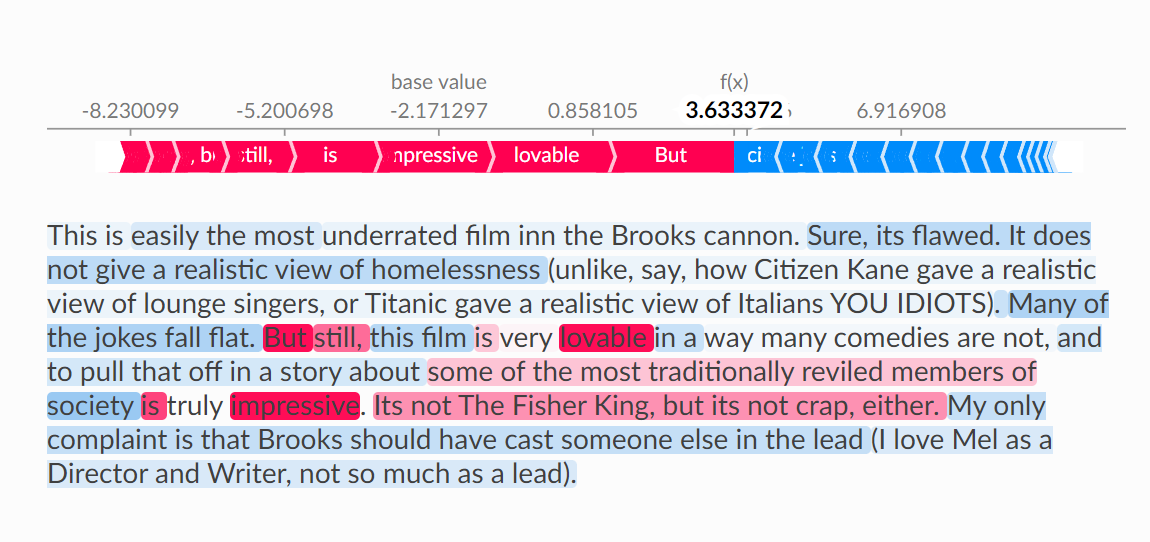
\includegraphics[width=0.8\ancho]{figs/shap_example.png}
    \caption{Ejemplo de visualización \citep{SHAPtextplot}}
    \label{fig:shap-ex}
\end{figure}

El color rojo indica tendencia a la clase positiva y el azul a la clase negativa. A partir del \textit{base value} y $f(x)$ indicados en el eje de la parte superior, podemos conocer cuál es el resultado de la clasificación comparándolos: si $f(x) > \textit{base value}$ la clasificación será positiva, mientras que si $f(x) < \textit{base value}$ será negativa. Por último, podemos ver la contribución de cada token en ambas partes: en la parte superior, el tamaño de los tokens varía según importancia o contribución a la clasificación; en la parte inferior esta relación se representa usando la intensidad de color, mayor intensidad indica mayor importancia.

Partiendo de estas nociones, podemos analizar el `razonamiento'\ de estos modelos utilizando ejemplos de noticias del conjunto de test, mostrando algunos ejemplos representativos.

\subsection{Politifact-Snopes One Evidence}

\begin{figure}[!h]
    \captionsetup[subfigure]{justification=Centering}

    % DistilBERT BASE (CASED / CASED MULTILINGUAL)
    \begin{subfigure}[t]{0.4\textwidth}
        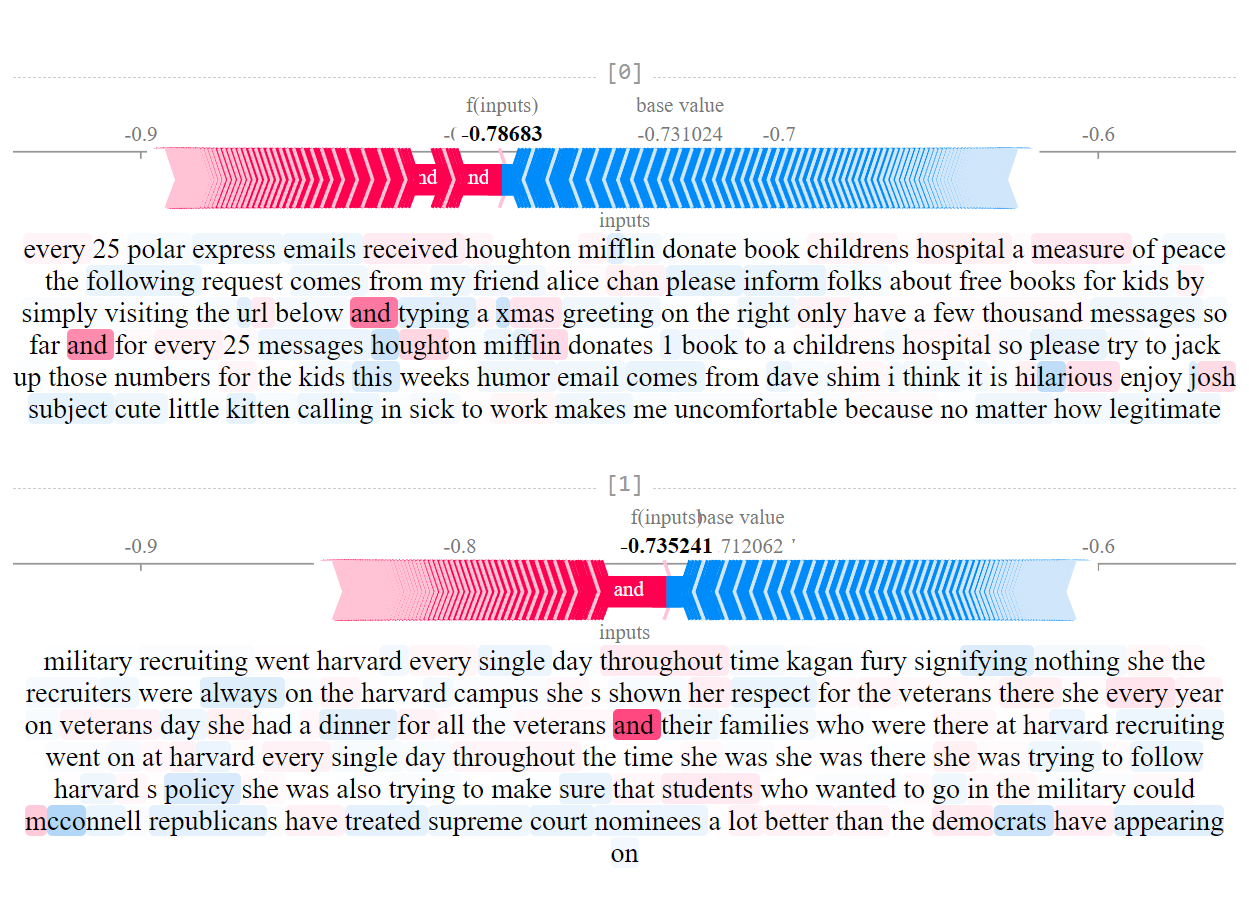
\includegraphics[width=\textwidth]{figs/one_TF/distil-b-c.png}
        \caption{{DistilBERT}\textsubscript{B, C}}
    \end{subfigure}
    \hspace{\fill} % maximize horizontal separation
    \begin{subfigure}[t]{0.4\textwidth}
        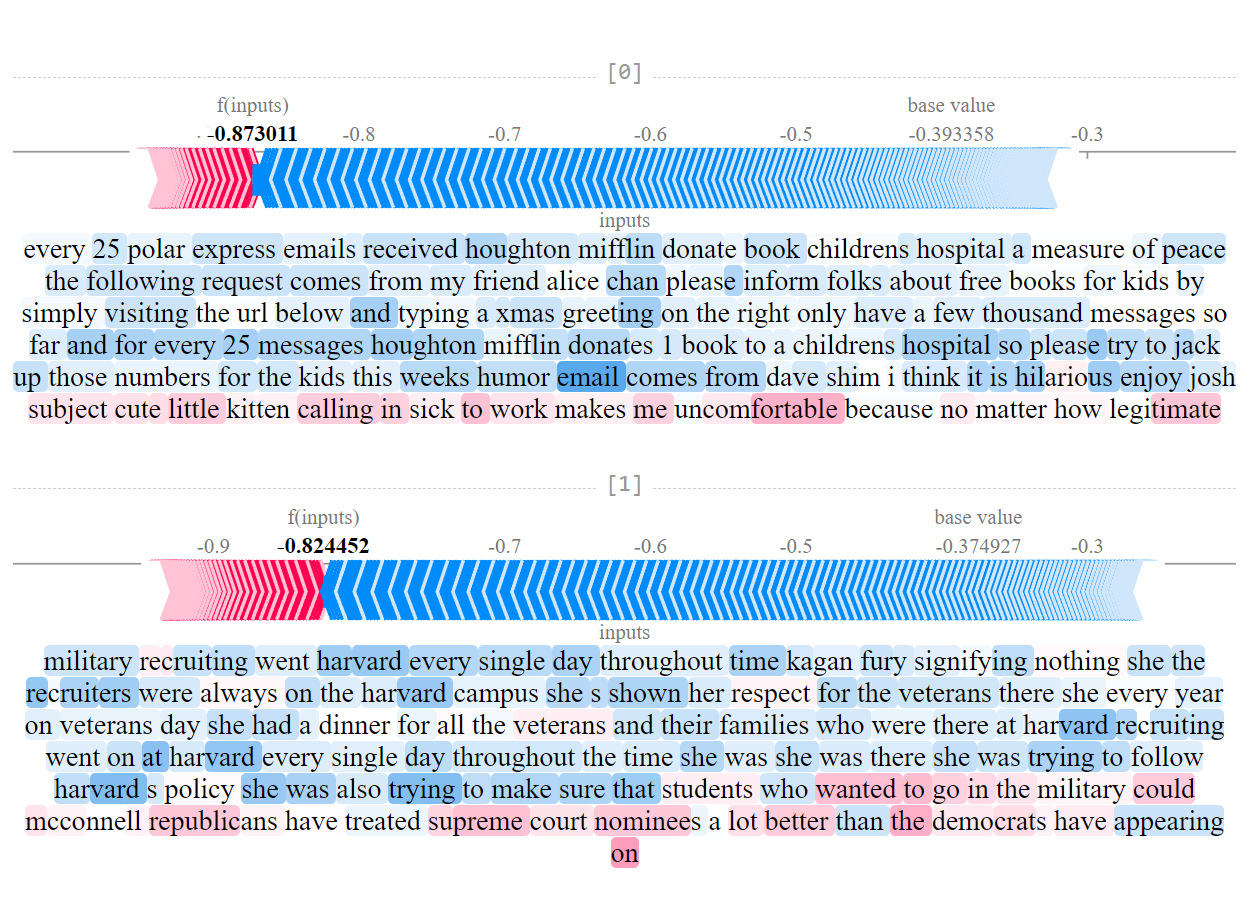
\includegraphics[width=\linewidth]{figs/one_TF/bert-b-ml-c.png}
        \caption{{DistilBERT}\textsubscript{B, C, ML}}
    \end{subfigure}
    
    \caption{Valores Shapley de cada modelo para dos noticias: una verdadera y una falsa del \textit{dataset} {P-S}\textsubscript{One}. Los subíndices utilizados para cada modelo $M$ indican respectivamente $M_{\text{B}}$: BASE; $M_{C}$: CASED; $M_{\text{ML}}$: MULTILINGUAL.}
    \label{fig:shap-ps-one}
\end{figure}

En este caso la primera noticia (superior) es verdadera, mientras que la segunda (inferior) falsa. Observamos que en ambos casos, los dos modelos tienden a la clase negativa en mayor o menor medida. 

Centrándonos en los ejemplos de la figura \hyperref[fig:shap-ps-one]{6.2} vemos que {DistilBERT}\textsubscript{B, C, ML} tiene una distribución de los valores Shapley más uniforme que en {DistilBERT}\textsubscript{B, C}. Parece que {DistilBERT}\textsubscript{B, C, ML} `presta más atención'\ a los \textit{tokens} individuales y menos a los colindantes. Esto nos puede dar la intuición de que este modelo parece `entender'\ el texto en general y por consecuencia, entender el estilo o la estructura sintáctica. 

También podemos hipotetizar que este comportamiento se debe al hecho de que este dataset no tiene ningún signo de puntuación ni capitalización, por lo que en el caso de los modelos CASED no pueden hacer uso de todas estas features para clasificar las noticias.

Analizando el comportamiento de los demás modelos (véase Apéndice \hyperref[fig:shap-ps-one-annex]{A.2.1.}), observamos que esta tendencia es parecida para {BERT}\textsubscript{B, C, ML}; {BERT}\textsubscript{L, U}; {BERT}\textsubscript{L, C}; {RoBERTa}\textsubscript{L} y {DeBERTa}\textsubscript{B}. Por otro lado, también encontramos otros modelos como {BERT}\textsubscript{B, U, ML}; {RoBERTa}\textsubscript{B} y {DeBERTa}\textsubscript{L} que prácticamente no parecen `prestar atención'\ a ningún token del texto. En estos casos los valores de \textit{base value} y $f(x)$ \textit{(logits)} también son muy similares, por lo que pensamos que con estos ejemplos los modelos no son capaces de encontrar las \textit{features} que caracterizan o no una \textit{fake news}.

En conclusión, observamos que algunos de los modelos parecen ser sensibles a estructuras más complejas que el \textit{token} individual, ya que la atención o la importancia de estos \textit{tokens} está más repartida a lo largo de la frase. Aún así, estos resultados no parecen ser concluyentes porque esa atención no está distribuida equitativamente a lo largo de la frase y tampoco el modelo consigue clasificar correctamente estos fragmentos.

\subsection{Politifact-Snopes All Evidences}

\begin{figure}[!h]
    \captionsetup[subfigure]{justification=Centering}
  \captionsetup[subfigure]{justification=Centering}

    % BERT BASE MULTILINGUAL (UNCASED / CASED)
    \begin{subfigure}[t]{0.4\textwidth}
        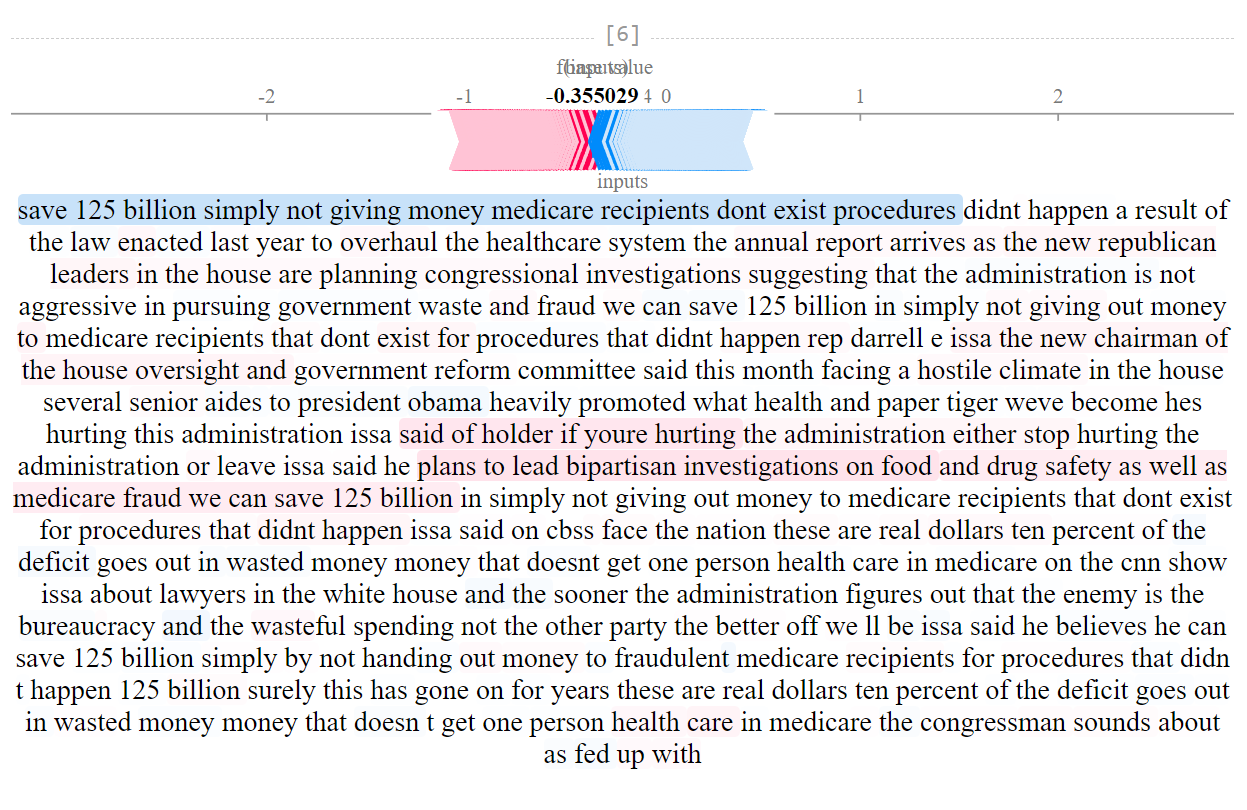
\includegraphics[width=\textwidth]{figs/all_F/bert-b-ml-u.png}
        \caption{{BERT}\textsubscript{B, U, ML}}
    \end{subfigure}
    \hspace{\fill} % maximize horizontal separation
    \begin{subfigure}[t]{0.4\textwidth}
        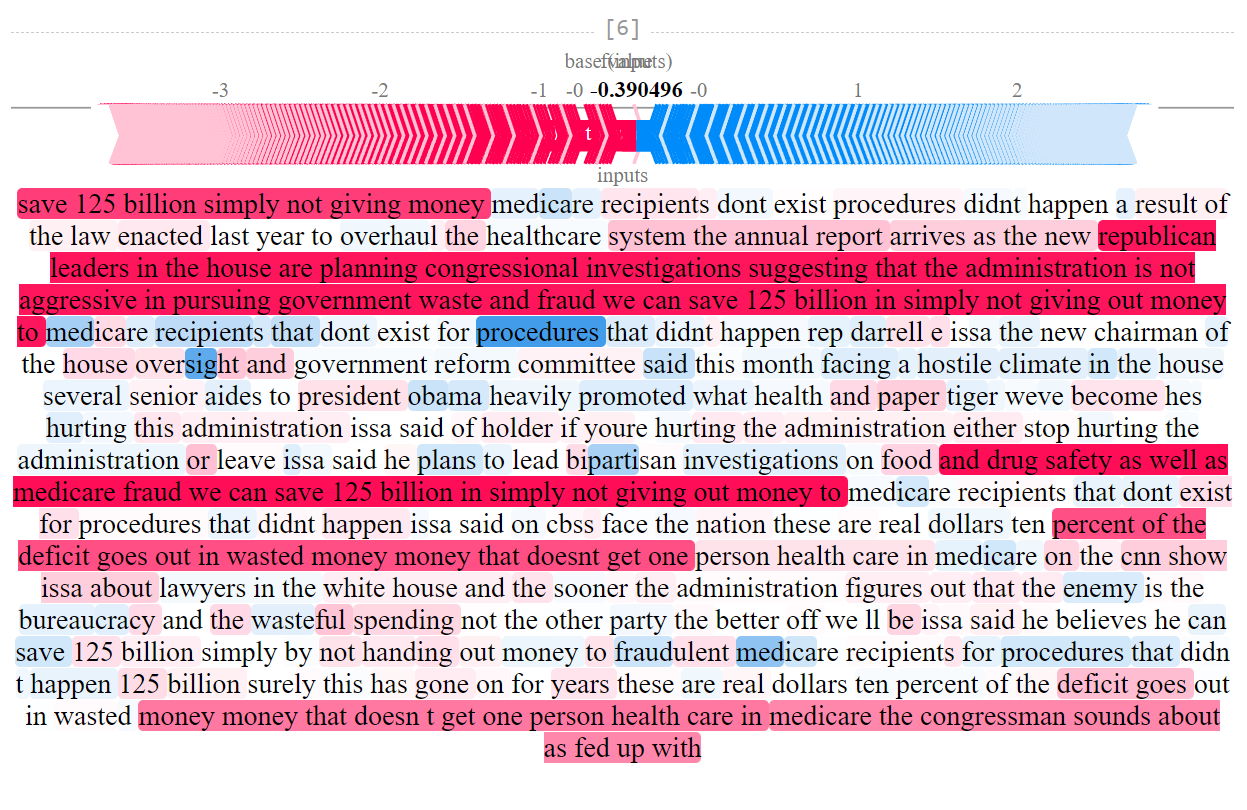
\includegraphics[width=\linewidth]{figs/all_F/bert-b-ml-c.png}
        \caption{{BERT}\textsubscript{B, C, ML}}
    \end{subfigure}  
    
    \caption{Valores Shapley de cada modelo para una noticia falsa del \textit{dataset} {P-S}\textsubscript{All}. Los subíndices utilizados para cada modelo $M$ indican respectivamente $M_{\text{B}}$: BASE; $M_{C}$: CASED; $M_{\text{U}}$: UNCASED; $M_{\text{ML}}$: MULTILINGUAL.}
    \label{fig:shap-ps-all}
\end{figure}

El ejemplo elegido es de una noticia falsa o \textit{fake news}, en la figura \hyperref[fig:shap-ps-all]{6.3} notamos que {BERT}\textsubscript{B, C, ML} parece `prestar atención' a estructuras más complejas que en el caso anterior. Leyendo las partes subrayadas con más intensidad nos da a entender que el modelo está `entendiendo' frases. Concretamente, estas frases son ``save 125 billion simply not giving money'', ``(investigations on food) and drug safety as well as medicare fraud we can save 125 billion in simply not giving out money to (medicare recipients that dont exist'', ``(ten) percent of the deficit goes out in wasted money [...]''. Estas frases son muy concisas, característica clave de las \textit{fake news}.

Por otro lado, {BERT}\textsubscript{B, U, ML} presta muy poca atención en comparación con el ejemplo anterior, aunque de la poca atención que presta, parece hacerlo también en frases y no \textit{tokens} individuales. Aún así, en ambos casos el resultado de la clasificación no parece influir, ya que los \textit{base value} y $f(x)$ son muy parecidos.

Los demás modelos (véase Apéndice \hyperref[fig:shap-ps-all-annex]{A.2.2.}) parecen seguir la tendencia de {BERT}\textsubscript{B, C, ML}; resaltando frases concretas, estos son concretamente: {BERT}\textsubscript{B, U}; {DistilBERT}\textsubscript{B, C}; {DistilBERT}\textsubscript{B, C, ML}; {RoBERTa}\textsubscript{B} y {DeBERTa}\textsubscript{L}. Los \textit{logits} obtenidos, reflejados en el valor $f(x)$, generalmente son mayores a los \textit{base values}, por lo que las clasificaciones realizadas son correctas y con un cierto grado de confianza.

El resto, sigue el comportamiento de {BERT}\textsubscript{B, U, ML}; con poca o nula atención a frases. Los \textit{logits} también son muy similares a los \textit{base values}, por lo que no parece haber mucha confianza en la predicción.

\subsection{News}

\begin{figure}[!h]
    \captionsetup[subfigure]{justification=Centering}

    % RoBERTa (BASE / LARGE)
    \begin{subfigure}[t]{0.4\textwidth}
        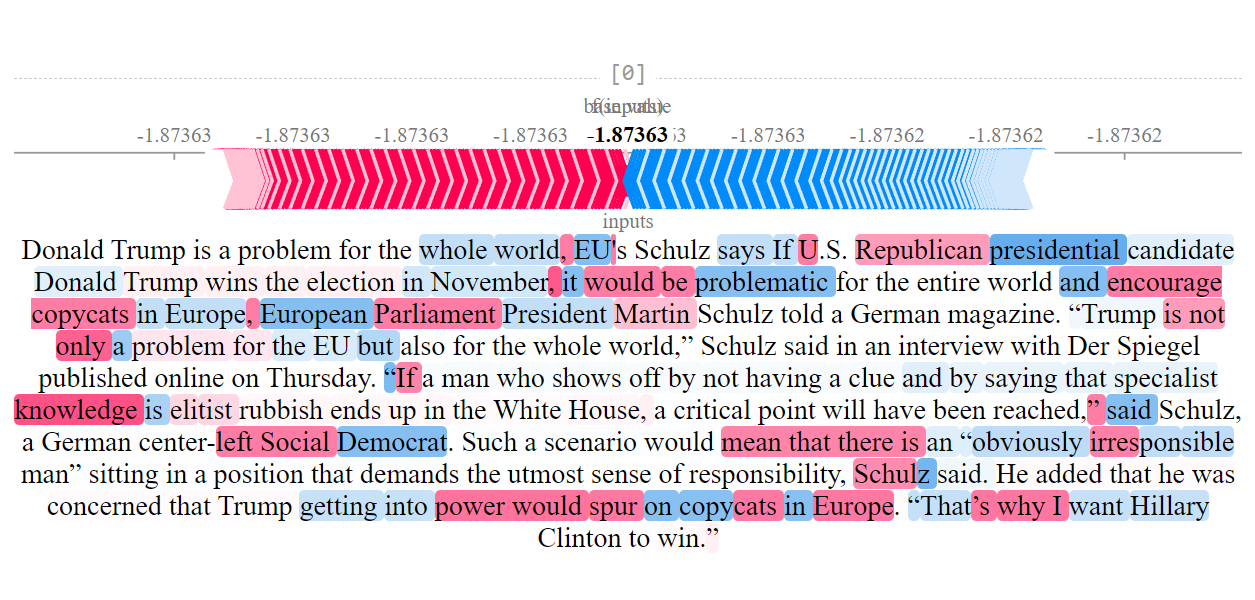
\includegraphics[width=\textwidth]{figs/news_T/roberta-b.png}
        \caption{{RoBERTa}\textsubscript{B}}
    \end{subfigure}
    \hspace{\fill} % maximize horizontal separation
    \begin{subfigure}[t]{0.4\textwidth}
        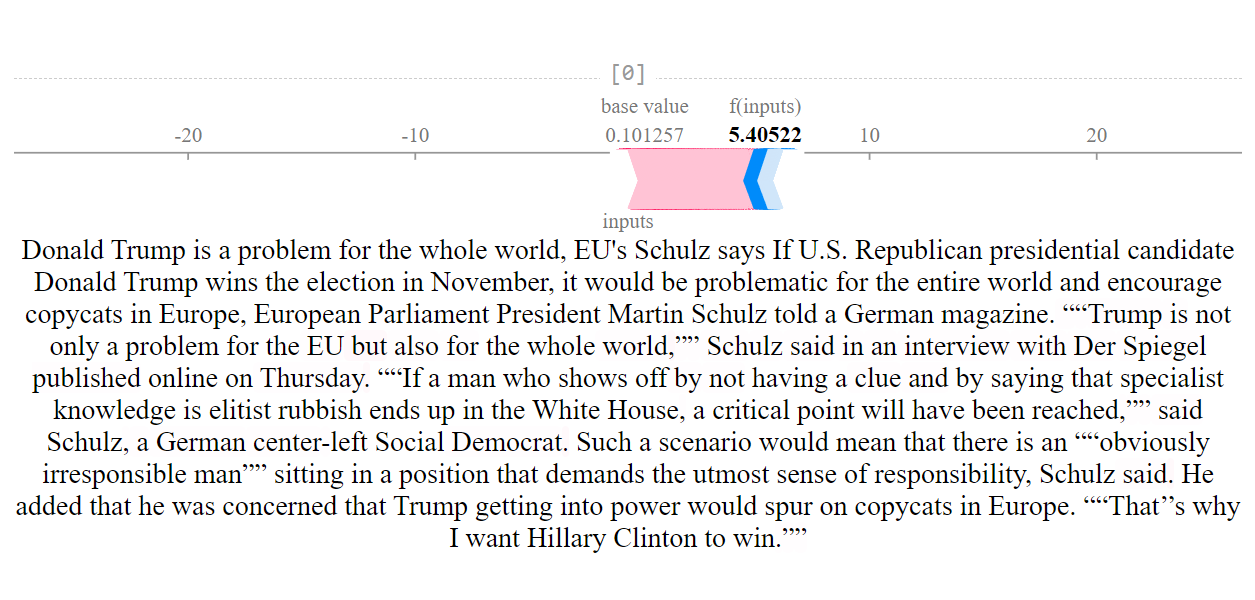
\includegraphics[width=\linewidth]{figs/news_T/roberta-l.png}
        \caption{{RoBERTa}\textsubscript{L}}
    \end{subfigure}
    
    \caption{Valores Shapley para una noticia verdadera del \textit{dataset} News. Los subíndices utilizados para cada modelo $M$ indican respectivamente $M_{\text{B}}$: BASE; $M_{\text{L}}$: LARGE.}
    
\end{figure}

Teniendo en cuenta que la noticia es verdadera, podemos observar que el peso de los \textit{tokens} para {RoBERTa}\textsubscript{B} son ínfimos en comparación con {RoBERTa}\textsubscript{L}. Este último modelo no parece resaltar ningún token como relevante para hacer la predicción. 

Este ejemplo no es aislado, esta tendencia es común a los siguientes modelos: {BERT}\textsubscript{B, U}; {BERT}\textsubscript{B, C, ML}; {BERT}\textsubscript{L, C}; {DistilBERT}\textsubscript{B, C}; {DistilBERT}\textsubscript{B, C, ML}; {RoBERTa}\textsubscript{L}; {DeBERTa}\textsubscript{B} y {DeBERTa}\textsubscript{L}. Solamente cuatro modelos de doce parecen al menos `razonar'\ y prestan atención a tokens concretos. Aún así, este `razonamiento'\ que tienen los otros modelos no parece tener mucho sentido tampoco, ya que suelen prestar atención a tokens sueltos y no a estructuras sintácticas concretas, cosa que no esperábamos.

Estos modelos parecen funcionar peor con este dataset que en los casos anteriores: la atención está muy distribuida de forma muy poco uniforme, los \textit{logits} tienen valores muy bajos en relación a los \textit{base values} o son extremadamente mayores (esto sucede en la mayoría de modelos que `no prestan atención'\ a ninguno de los \textit{tokens} en el texto.

\section{Evaluación}
\label{sec:eval}

Habiendo analizado los resultados en la sección \hyperref[sec:results]{6.1}, podemos deducir que los modelos entrenados no parecen funcionar correctamente para detectar \textit{fake-news} gracias a sus características estilísticas. Aún así, viendo las métricas de \textit{specificity}, creemos que mediante esta metodología hemos creado un sistema capaz de detectar las \textit{features} que hacen que una noticia sea verdadera, concretamente los modelos LARGE, {DistilBERT}\textsubscript{B, C, ML}; {BERT}\textsubscript{B, C} y {DeBERTa}\textsubscript{B} son los que ofrecen mejores métricas para los \textit{datasets} de PolitiFact-Snopes, siendo los modelos LARGE los más consistentes en todos los \textit{datasets}.

En la sección \hyperref[sec:shap]{6.2} hemos intentando entender cuál es el funcionamiento o razonamiento interno detrás de estos modelos a la hora de clasificar. Utilizando los valores Shapley, hemos modelizado la atención de estos modelos y mediante ellos determinar qué palabras o frases son las más importantes en la clasificación.

En general, los resultados no eran los esperados, ya que las métricas obtenidas en la sección \hyperref[sec:results]{6.1} nos daban una visión más optimista del rendimiento de estos modelos. El \textit{dataset} con el que hemos obtenido el mejor rendimiento ha sido {P-S}\textsubscript{All}, el siguiente {P-S}\textsubscript{One} y el peor News.

Es por ello que creemos que es necesario investigar en profundidad otros factores resaltados en la sección \hyperref[sec:results]{6.1}, como la pérdida de rendimiento general de los modelos BASE al añadir más evidencias o al entrenar con el \textit{dataset} News, o en la sección \hyperref[sec:shap]{6.2}, como los mecanismos de atención de estos modelos y el pobre funcionamiento con el \textit{dataset} News.

\chapter{Discusión}
\label{chapter:7}
\section{Explicabilidad de los modelos}
\label{sec:expl}

El artículo de \citet{Dillon2021} recalca que hay que tener cuidado al interpretar los resultados obtenidos mediante técnicas como SHAP en búsqueda de conclusiones causales, ya que estas pueden ser erróneas o basarse en hechos infundados. Debido a que los modelos predictivos asumen ciertos comportamientos iguales en el futuro, los esquemas de correlación también se mantendrán constantes.

La revisión de \citet{Mosca2022} introduce otras técnicas basadas en valores Shapley, como \textit{L-Shapley} o \textit{C-Shapley}, y comenta críticas de otros trabajos hacia el uso en general del uso de valores Shapley en modelos de lenguaje que debatiremos a continuación.

\citet{Kumar2020} muestra que usar los valores Shapley puede provocar inconsistencias, las cuales añaden complexidad a los modelos que intentan mitigarlas. \citet{Merrick2019} critica la poca justificación o explicación en la incertidumbre en las explicaciones producidas mediante valores Shapley. En este caso muestran como pequeñas diferencias pueden generar efectos sobredimensionados en los resultados obtenidos, incluso en \textit{features} que no tienen relevancia en el modelo.

Cabe recalcar que estos trabajos no están directamente aplicados a tareas de Procesado de Lenguaje Natural. Aún así, consideramos necesario tener en cuenta estas perspectivas para contextualizar sobre todas los factores que influyen en el análisis de los resultados.

\section{Limitaciones de los modelos}

El trabajo de \citet{Rogers2020} ilustra los todos los conocimientos que se saben con respecto a los modelos basados en BERT en diferentes ámbitos.

\textbf{Conocimiento sintáctico.} BERT no `entiende'\ las negaciones y no es sensible al texto con una sintaxis incorrecta (orden de palabras aleatorizado, frases truncadas, sujetos o objetos eliminados \citep{Ettinger2019}

\textbf{Conocimiento semántico.} BERT tiene dificultades a la hora de trabajar con dígitos. Esto es problema del tokenizador WordPiece, que puede dividir números de valores similares de formas muy diferentes, afectando a todos los pasos posteriores del procesamiento y finalmente al resultado.

\textbf{Sentido común.} BERT no consigue llevar a cabo tareas de inferencia pragmática correctamente \citep{Ettinger2019} ni razonar a partir de su conocimiento del mundo \citep{Forbes2019, Zhou2019, Richardson2019}

Estos puntos mencionados dificultan el desarrollo de aplicaciones basadas en estas familias de modelos, concretamente el entrenamiento de modelos basado en hechos, ya que BERT tiene dificultades en el razonamiento. Aunque nuestra aplicación esté basada en características estilísticas, creemos que la falta de sensibilidad hacia las negaciones, estructuras sintácticas incorrectas o el problema a la hora de tratar con dígitos si que puede afectarnos en mayor o menor medida en los resultados obtenidos.


\section{Posibles sesgos}
\label{sec:biases}

En esta sección haremos una revisión bibliográfica sobre los trabajos realizados con respecto a determinar sesgos en LLMs.

\textbf{Word Embeddings estáticos y contextuales.} La investigación de \citet{Kurita2019} muestra que existen sesgos semánticos similares en \textit{word embeddings} contextuales al igual como sucede en los \textit{word embeddings} estáticos \citep{Caliskan2017}. Es más, el \textit{Word Embedding Associate Test} (WEAT) \citep{Caliskan2017}, no es directamente aplicable en estos modelos, debido a su naturaleza contextual. En el caso de aplicar esta métrica para reducir los sesgos en los modelos de lenguaje contextuales no es suficiente e incluso puede agravarlos aún más \citep{Silva2021}.

% \citet{Silva2021,Vig2020,Basta2019,Bommasani2020} han demostrado encontrar sesgos similares en este tipo de modelos basados en \textit{transformers}:

\textbf{Destilado de modelos.} Concretamente, los modelos destilados (en el caso de DistilBERT y DistilRoBERTa) muestran un sesgo estadísticamente mayor y más fuerte que en sus versiones no destiladas (BERT y RoBERTa) \citep{Silva2021}. Esto está en línea de los hallazgos de \citet{Hooker2020}, que encuentran que el proceso de destilado de modelos de visión daña desproporcionadamente a grupos minorizados. Aunque los trabajos de \citet{Gilburt2019,TanCelis2019} concluyen que aumentar el tamaño del modelo conlleva una reducción en el sesgo, \citet{Silva2021,Nadeem2021} demuestran lo contrario.

\textbf{Tokenización.} La tokenización es también crucial a la hora de desvelar sesgos: los modelos \textit{uncased}, es decir los que no distinguen entre palabras capitalizadas y no capitalizadas suelen mostrar menos sesgos y por lo tanto mayor diversidad con respecto a nombres y pronombres \citep{Silva2021}

\textbf{Modelos aumentados.} Mediante el trabajo de \citet{Vig2020}, podemos vislumbrar que los LLMs, concretamente las versiones aumentadas (véase las versiones LARGE de los modelos tratados a lo largo de este trabajo) tienen mayor capacidad de `sintetizar'\ o adquirir sesgos, aunque estos se manifiestan en una pequeña proporción de neuronas o \textit{attention heads}. El análisis cuantitativo desempeñado muestra que pueden existir componentes en estos modelos `encargados'\ explícitamente de reproducir sesgos o prejuicios (concretamente en este estudio solo se tratan estereotipos de género).

En conclusión, en este trabajo utilizamos modelos pre-entrenados basados en BERT, los cuales están demostrados que están sesgados. Es por ello que hay que tener en consideración para futuras investigaciones todos los factores que afectan al sesgo de los modelos para intentar reducirlo o en el caso de que no sea posible, tenerlo en cuenta en el análisis de los resultados.

\chapter{Conclusiones}
\label{chapter:8}
A continuación vamos a analizar cómo se han cumplido cada uno de los objetivos propuestos en la sección \hyperref[sec:objetivos]{1.2}:

\textbf{Definir correctamente el término \emph{fake news} y delimitar el área de estudio a tratar.} En el capítulo \hyperref[sec:defs]{2} hemos hecho una revisión bibliográfica, tomando diferentes definiciones del término y analizando los diferentes matices que aportan cada uno, decantándonos finalmente por el término de \textit{disinformation}, trabajando solamente noticias. Sabemos que nos dejamos muchas otras formas de \textit{disinformation}, pero es inevitable hacerlo debido a la naturaleza del Trabajo de Fin de Grado, es por ello que instamos a seguir investigando en el tema.

\textbf{Desarrollar una solución que permita clasificar noticias, sirviendo como triaje en el proceso de \textit{fact-checking}.} Se han propuesto diferentes modelos de lenguaje y \textit{datasets} y, viendo los resultados obtenidos en la sección \hyperref[sec:results]{6.1}, consideramos que hemos desarrollado un clasificador de noticias aunque los resultados no han sido los esperados. Los modelos LARGE, {DistilBERT}\textsubscript{B, C, ML}; {BERT}\textsubscript{B, C} y {DeBERTa}\textsubscript{B} son los que mejor funcionan en este problema, aunque creemos que los modelos implementados destacan más por sus métricas de \textit{specificity}, es decir, por su capacidad de distinguir qué características destacan en las noticias verdaderas. Aún así, por las métricas obtenidas en general, hace falta más trabajo para desarrollar una implementación que sea competente en el estado del arte actual.

\textbf{Hacer un estudio comparativo de los diferentes factores de los modelos y su aprendizaje, analizando la forma en la que afectan a su rendimiento.} En el capítulo \hyperref[chapter:6]{6} hemos comparado los diferentes resultados obtenidos y buscado una justificación plausible a este comportamiento. A grandes rasgos, el tamaño del modelo es el factor que parece contribuir más a la mejora de rendimiento de este. Lo segundo que parece afectar más es el hecho de si el modelo es multilingüe o distingue entre palabras capitalizadas. Por último, el tamaño del \textit{dataset} parece ser lo que menos contribuye, aunque hay que considerar la capacidad de generalización del modelo.

\textbf{Aplicar técnicas de \textit{Explainable AI} para entender el funcionamiento interno de los modelos en el proceso de clasificación.} En la sección \hyperref[sec:shap]{6.2} aplicamos estas técnicas mediante la librería \texttt{shap} y, mediante los valores Shapley, modelizamos la atención o la importancia que le da el modelo a ciertos \textit{tokens} en la clasificación. Concluimos que el comportamiento que tienen estos modelos no es el esperado, funcionando mejor en los \textit{datasets} {P-S}\textsubscript{One} y {P-S}\textsubscript{All} con menor información y número total de muestras que News. 
\newpage
\textbf{Analizar como afectan los sesgos en esta familia de modelos a los resultados obtenidos.} Como hemos observado en el apartado \hyperref[sec:biases]{7.2}, gracias a una revisión bibliográfica hemos conseguido desvelar sesgos en los LLMs. Estos no solo se limitan a una representación como \textit{word embedding} que puede dar interpretación a sesgos o prejuicios, sino que prácticamente estos sesgos son inherentes al proceso de aprendizaje. Es por ello que hay que tener en cuenta todos estos factores para realizar un análisis correcto de los resultados y de esta forma evitar perpetuando estos sesgos de forma directa e indirecta.

\chapter{Trabajos futuros}
Como posibles mejoras para aplicar a la metodología aplicada se sugieren las siguientes propuestas:
\begin{itemize}
    \item Probar arquitecturas diferentes a la familia BERT, analizando su efecto en los resultados obtenidos. Un ejemplo puede ser ELECTRA \citep{Clark2020}, utilizado en el trabajo de \citet{Wang2021}.
    \item Probar a entrenar los modelos un número mayor de épocas, implementando un mecanismo de \textit{early stopping}.
    \item Realizar el experimento con \textit{datasets} de noticias de diferentes características: mayor variedad de temas y estilos de escritura, diferencias en longitud de los textos, etc.
    \item Añadir más categorías o \textit{labels} en la clasificación, como sátira.
    \item Aplicar otras técnicas de \textit{Explainable AI}, como puede ser LIME.
\end{itemize}

Con respecto a nuevas líneas de investigación, se esbozan las siguientes ideas:
\begin{itemize}
    \item Implementar \textit{Multi-task Learning} o Aprendizaje Semi-supervisado, ya que hay indicios de ayudar en el proceso de aprendizaje y mejorar la clasificación \citep{Rei2017}. \citet{Wang2021} tiene una aplicación similar para clasificación de mensajes en situación de desastres.
    \item Generar un dataset priorizando la calidad de las noticias frente a la cantidad, similar al trabajo desarrollado por \citet{Gunasekar2023}
\end{itemize}


\nocite{*}

\pagestyle{bib}
% \chapter*{Bibliografía}
\addcontentsline{toc}{chapter}{Bibliografía}
\printbibliography
\label{Bibliografía}
% \bibliographystyle{apalike}
% \bibliography{bib/bibliografia.bib}

\pagestyle{appendix}
\appendix
\chapter{Apéndice}
\section{Fragmentos originales}
\subsection{Fragmento 1}
\label{frag1eng}
\begin{quotation}
    \emph{``news articles that are intentionally and verifiably false, and could mislead readers''} --- \hyperref[frag1esp]{Fragmento en castellano}
\end{quotation}

\subsection{Fragmento 2}
\label{frag2eng}
\begin{quotation}
    \emph{``fabricated information that mimics news media content in form but not in organisational process or intent''} --- \hyperref[frag2esp]{Fragmento en castellano}
\end{quotation}

\subsection{Fragmento 3}
\label{frag3eng}
\begin{quotation}
    \emph{``fake news appropriates the look and feel of real news; from how websites look; to how articles are written; to how photos include attributions. Fake news hides under a veneer of legitimacy as it takes on some form of credibility by trying to appear like real news. Furthermore, going beyond the simple appearance of a news item, through the use of news bots, fake news imitates news’ omnipresence by building a network of fake sites.''} --- \hyperref[frag3esp]{Fragmento en castellano}
\end{quotation}

\subsection{Fragmento 4}
\label{frag4eng}
\begin{quotation}
    \emph{``Information is propositional content in that it proposes that a specific state of the world exists: it is `what must be the case in the world for the sign to exist as and when it does'.''} --- \hyperref[frag4esp]{Fragmento en castellano}
\end{quotation}

\subsection{Fragmento 5}
\label{frag5eng}
\begin{quotation}
    \emph{``\underline{Misinformation.} Propositional content of signs that misrepresents the state of the world without the intention to deceive [...]. One area where this [...] is quite common is health advice in online communities \citep{Venkatesan2014}, where many people spread false information unintentionally \citep{Myers2009}.''}  --- \hyperref[frag5esp]{Fragmento en castellano}
\end{quotation}

\subsection{Fragmento 6}
\label{frag6eng}
\begin{quotation}
    \emph{``\underline{Disinformation.} Propositional content of signs that misrepresents the state of the world with the intention to deceive.''}  --- \hyperref[frag6esp]{Fragmento en castellano}
\end{quotation}

\subsection{Fragmento 7}
\label{frag7eng}
\begin{quotation}
    \emph{``\underline{Malinformation.} Propositional content of signs that truthfully represents the state of the world with the intention to deceive [...] It is often assumed that deception appears in the form of or as result of bald-face lying and other forms of disinformation. However, deception can equally happen in the form or as a result of subtle manipulation of information that does not necessarily misrepresent the world but is intended to deceive \citep{McCornack2009,McCornack2014,Wardle2018a}. Examples include half-truths and spin, which refer to incomplete or selective information provided with the intention to deceive \citep{Fallis2016}.''} --- \hyperref[frag7esp]{Fragmento en castellano}
\end{quotation}

\clearpage
\section{Visualización SHAP}

\subsection{Politifact-Snopes One Evidence}
\label{fig:shap-ps-one-annex}

\begin{figure}[!ht]
    \captionsetup[subfigure]{justification=Centering}
    % BERT BASE (UNCASED / CASED)
    \begin{subfigure}[t]{0.4\textwidth}
        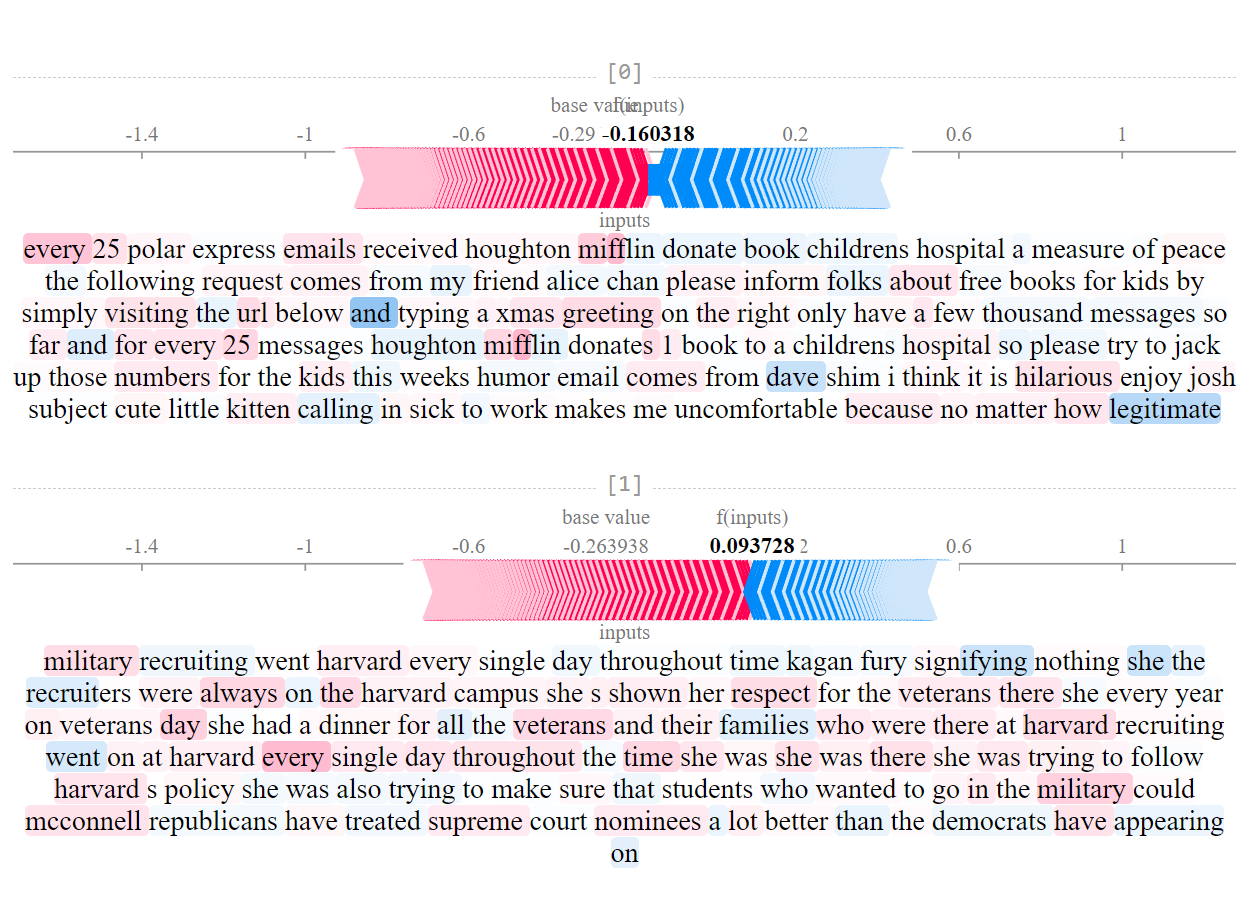
\includegraphics[width=\textwidth]{figs/one_TF/bert-b-u.png}
        \caption{{BERT}\textsubscript{B, U}}
    \end{subfigure}
    \hspace{\fill} % maximize horizontal separation
    \begin{subfigure}[t]{0.4\textwidth}
        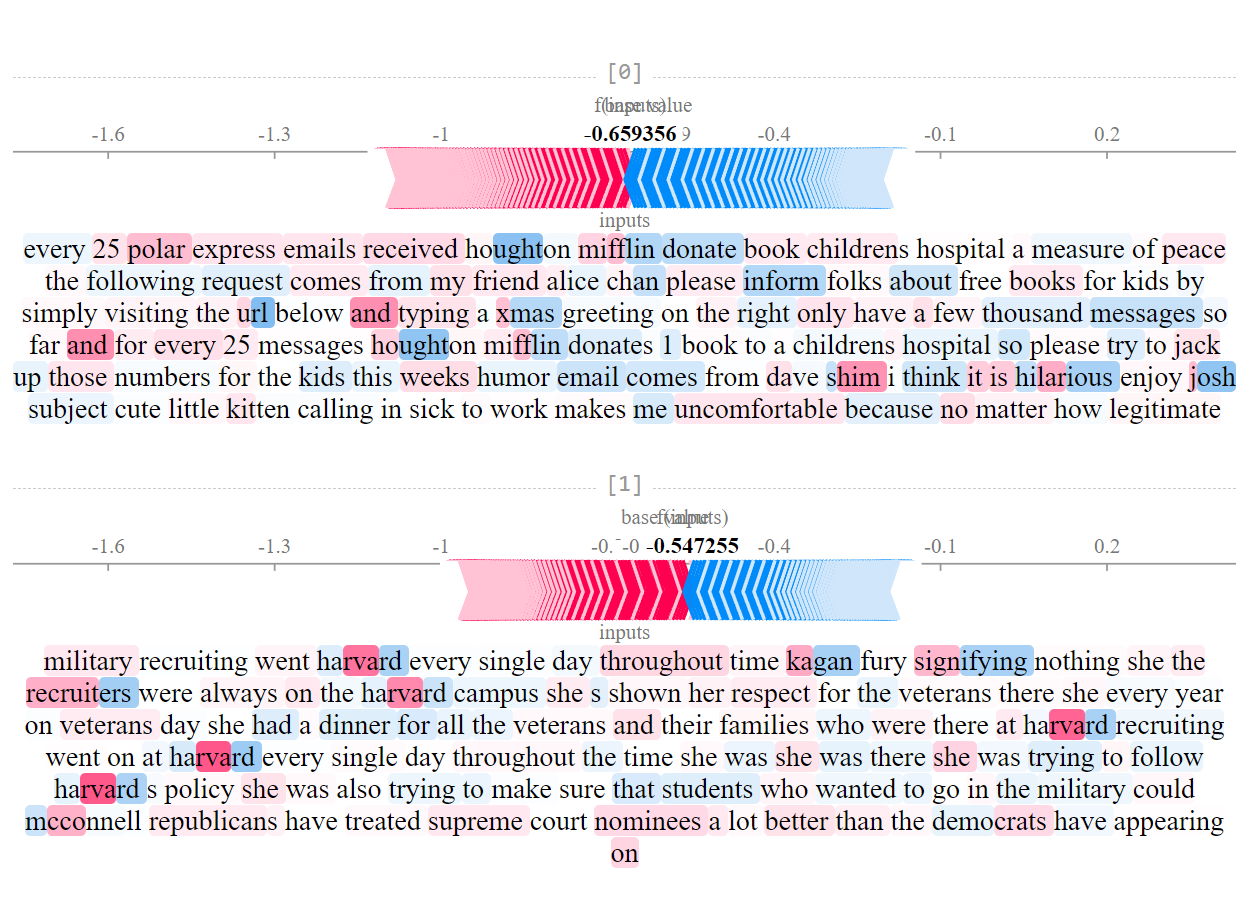
\includegraphics[width=\linewidth]{figs/one_TF/bert-b-c.png}
        \caption{{BERT}\textsubscript{B, C}}
    \end{subfigure}


% \end{figure}
% \begin{figure}[h]\ContinuedFloat
%     \captionsetup[subfigure]{justification=Centering}

    % BERT BASE MULTILINGUAL (UNCASED / CASED)
    \begin{subfigure}[t]{0.4\textwidth}
        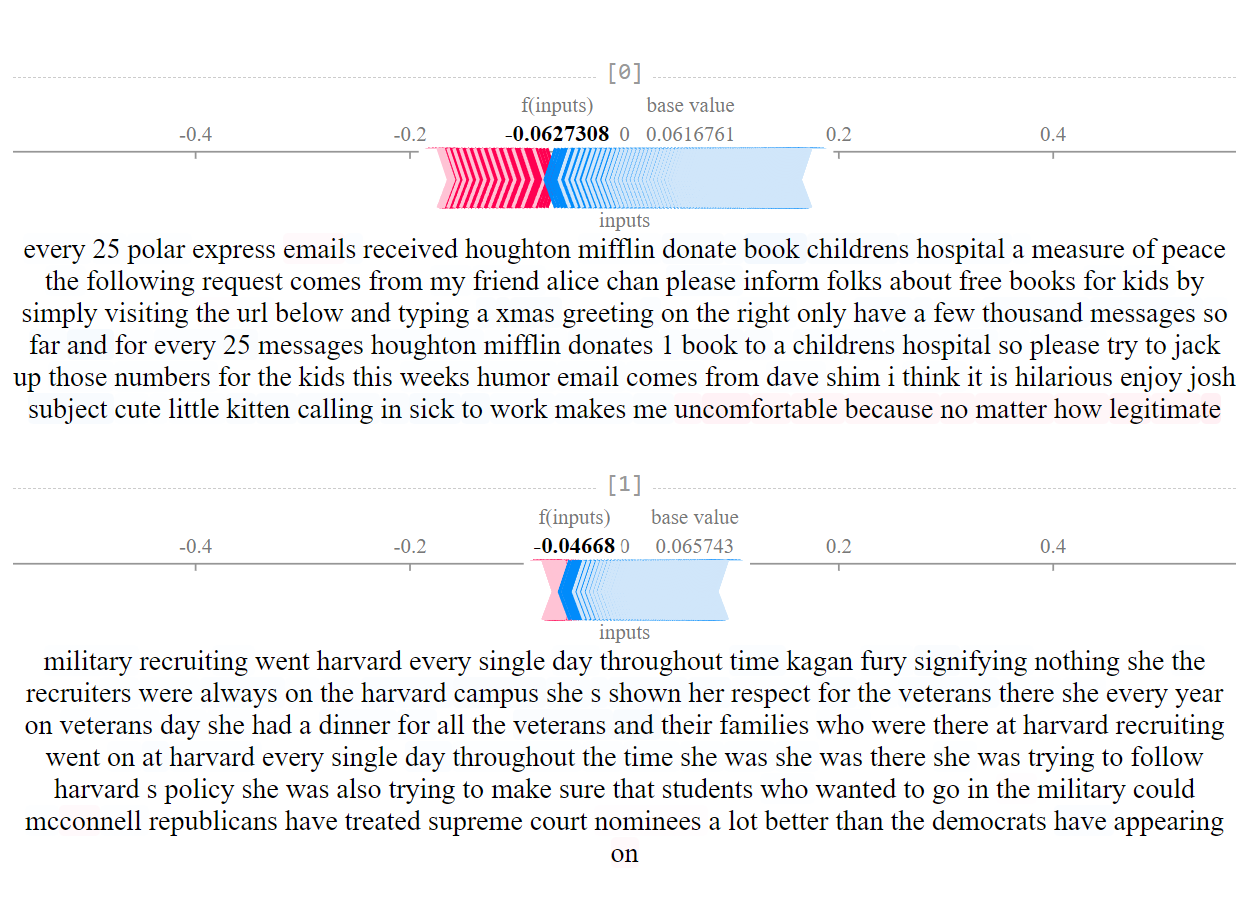
\includegraphics[width=\textwidth]{figs/one_TF/bert-b-ml-u.png}
        \caption{{BERT}\textsubscript{B, U, ML}}
    \end{subfigure}
    \hspace{\fill} % maximize horizontal separation
    \begin{subfigure}[t]{0.4\textwidth}
        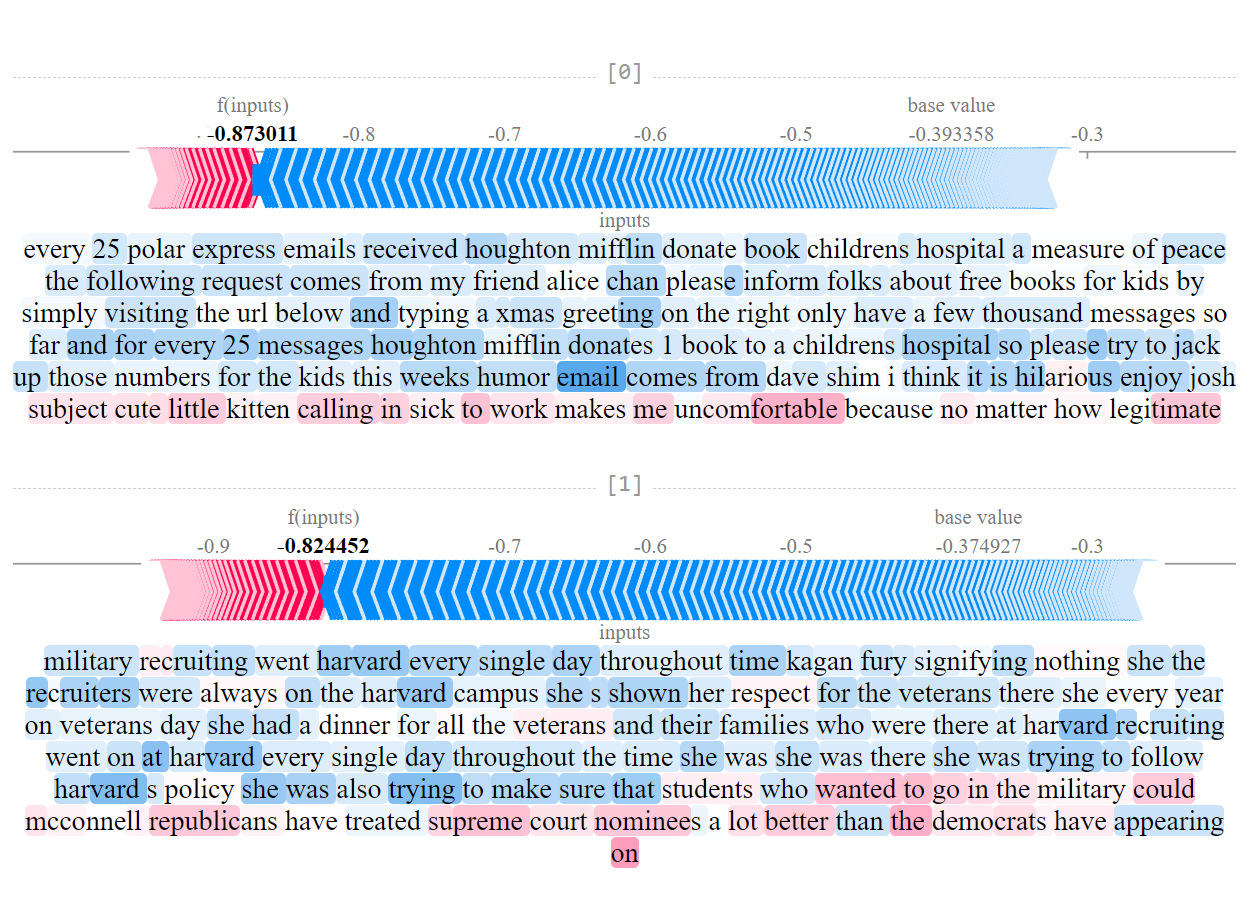
\includegraphics[width=\linewidth]{figs/one_TF/bert-b-ml-c.png}
        \caption{{BERT}\textsubscript{B, C, ML}}
    \end{subfigure}


% \end{figure}
% \begin{figure}[h]\ContinuedFloat
%     \captionsetup[subfigure]{justification=Centering}

    % BERT LARGE (UNCASED / CASED)
    \begin{subfigure}[t]{0.4\textwidth}
        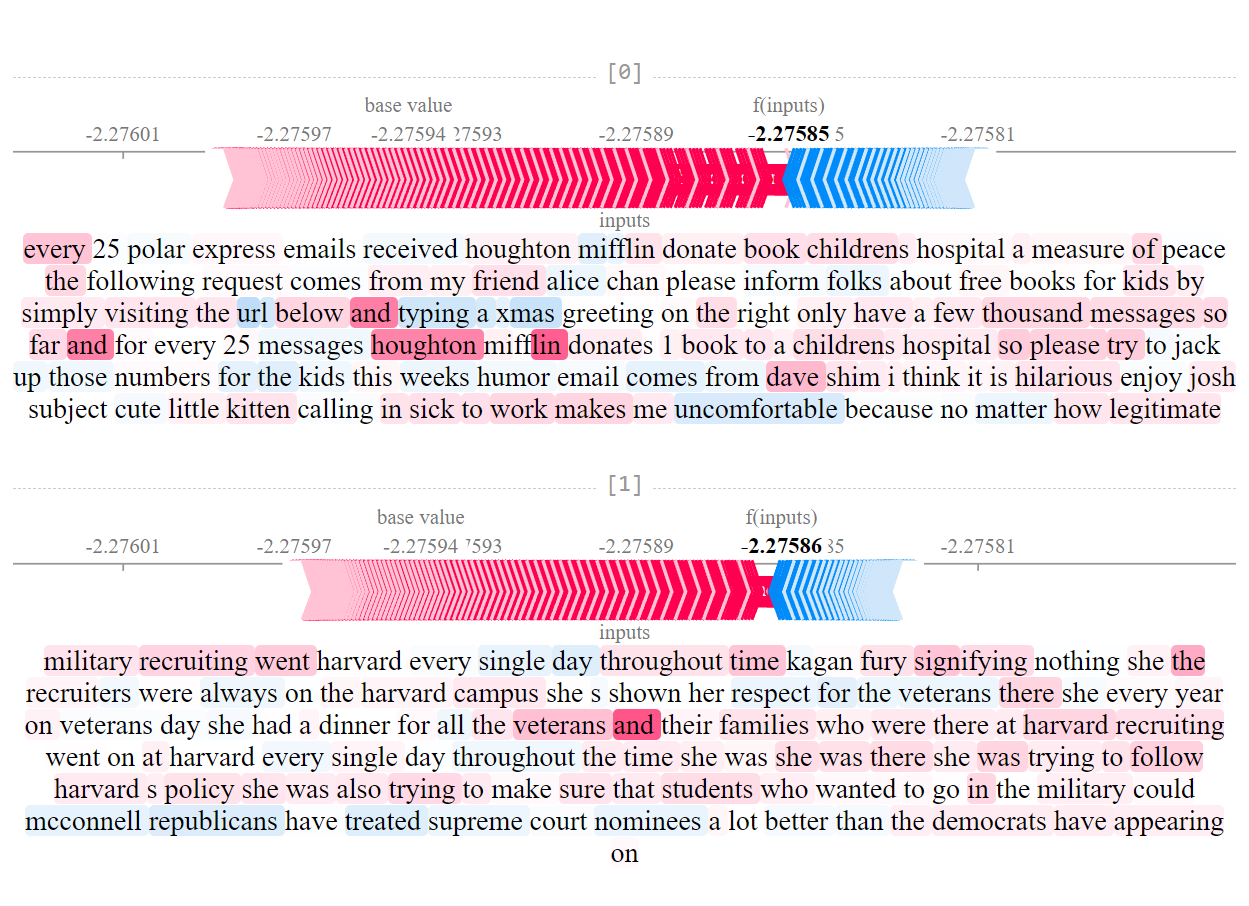
\includegraphics[width=\textwidth]{figs/one_TF/bert-l-u.png}
        \caption{{BERT}\textsubscript{L, U}}
    \end{subfigure}
    \hspace{\fill} % maximize horizontal separation
    \begin{subfigure}[t]{0.4\textwidth}
        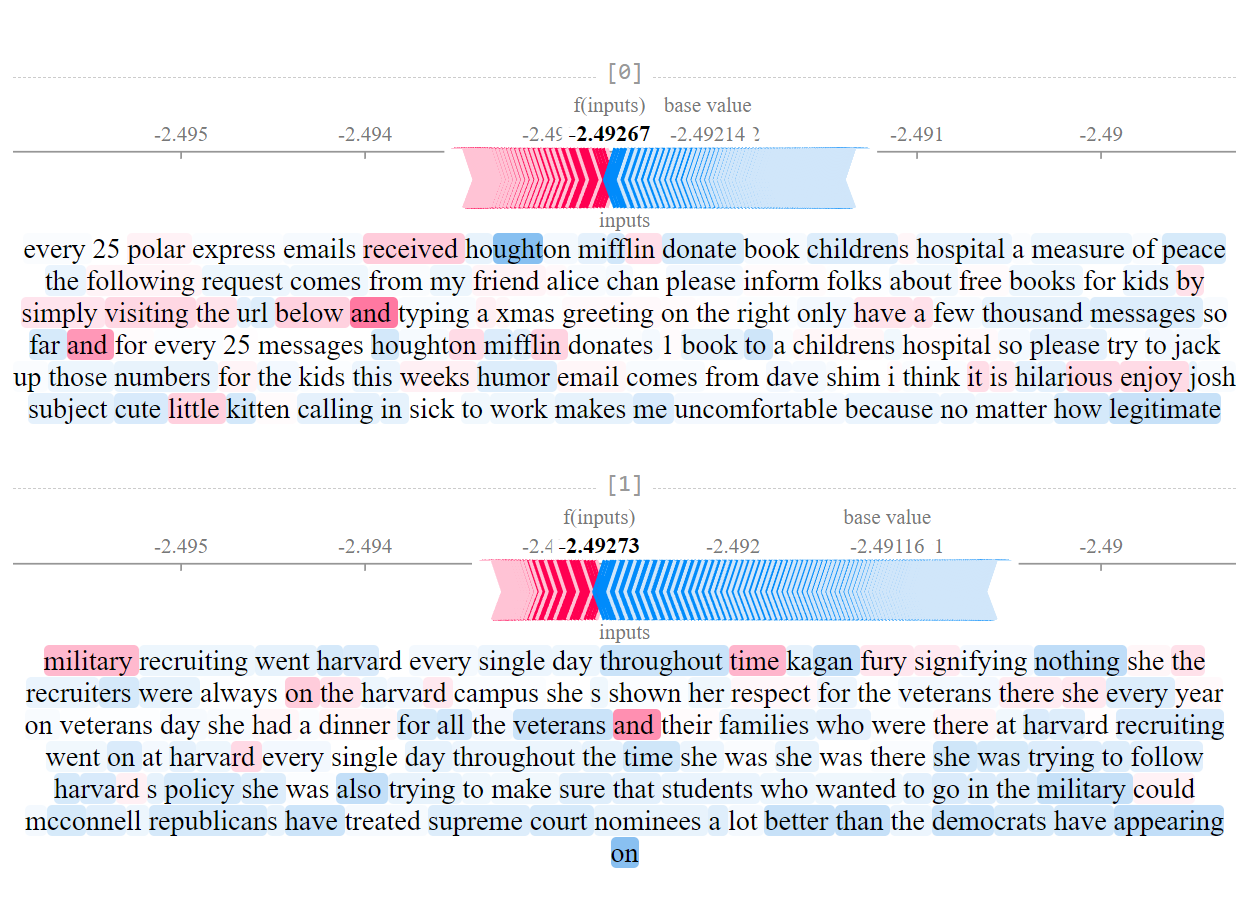
\includegraphics[width=\linewidth]{figs/one_TF/bert-l-c.png}
        \caption{{BERT}\textsubscript{L, C}}
    \end{subfigure}


% \end{figure}
% \begin{figure}[!ht]\ContinuedFloat
%     \captionsetup[subfigure]{justification=Centering}

    % DistilBERT BASE (CASED / CASED MULTILINGUAL)
    \begin{subfigure}[t]{0.4\textwidth}
        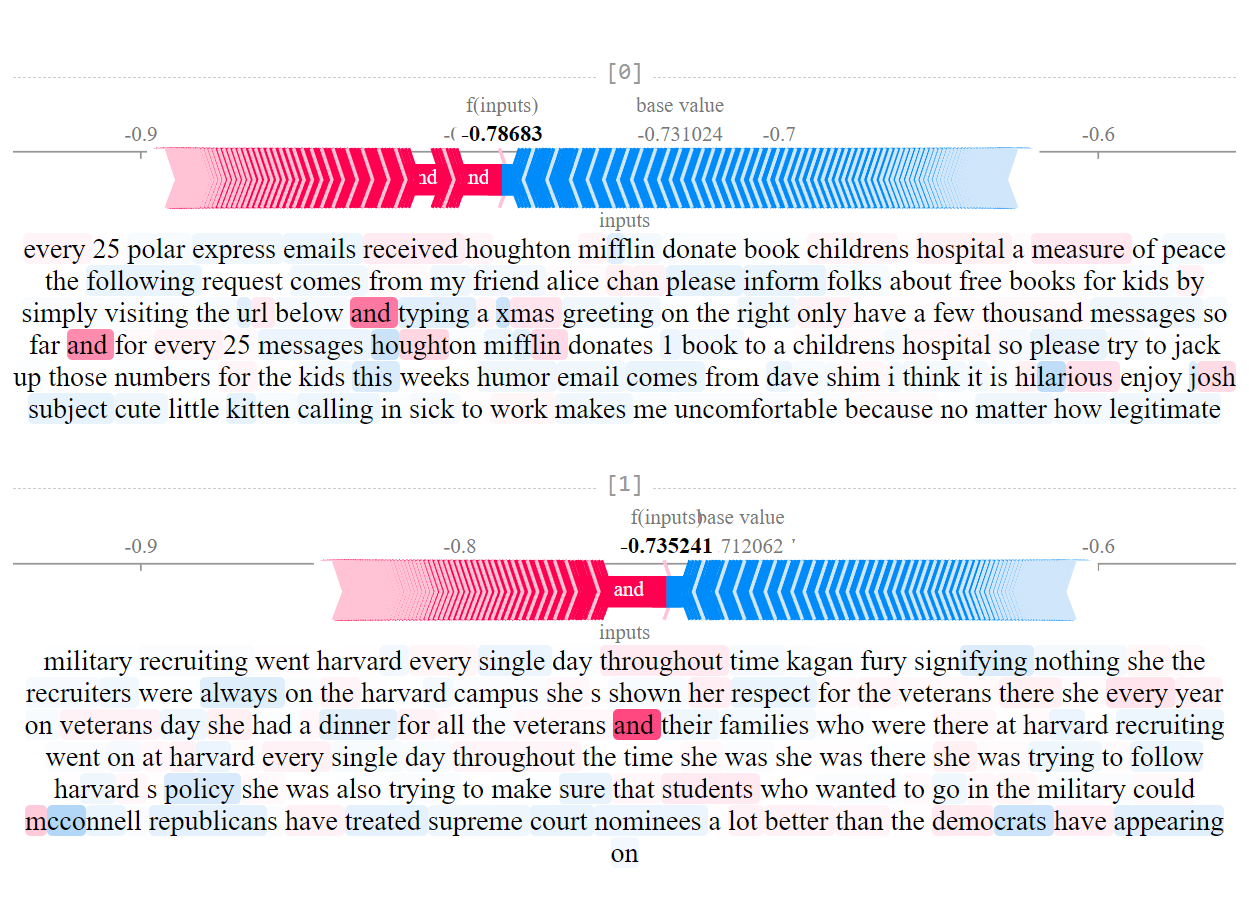
\includegraphics[width=\textwidth]{figs/one_TF/distil-b-c.png}
        \caption{{DistilBERT}\textsubscript{B, C}}
    \end{subfigure}
    \hspace{\fill} % maximize horizontal separation
    \begin{subfigure}[t]{0.4\textwidth}
        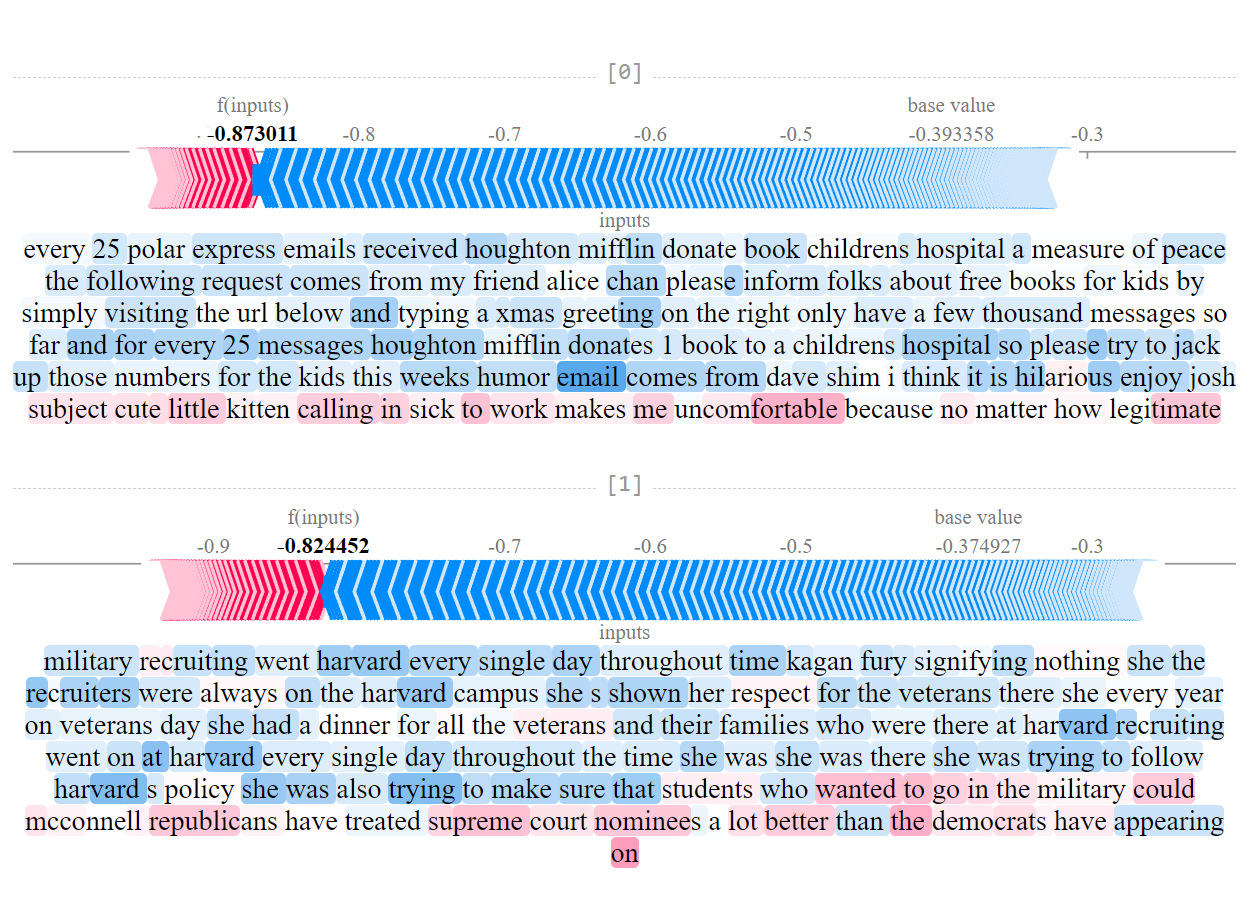
\includegraphics[width=\linewidth]{figs/one_TF/bert-b-ml-c.png}
        \caption{{DistilBERT}\textsubscript{B, C, ML}}
    \end{subfigure}


\end{figure}
\begin{figure}[!h]\ContinuedFloat
    \captionsetup[subfigure]{justification=Centering}

    % RoBERTa (BASE / LARGE)
    \begin{subfigure}[t]{0.4\textwidth}
        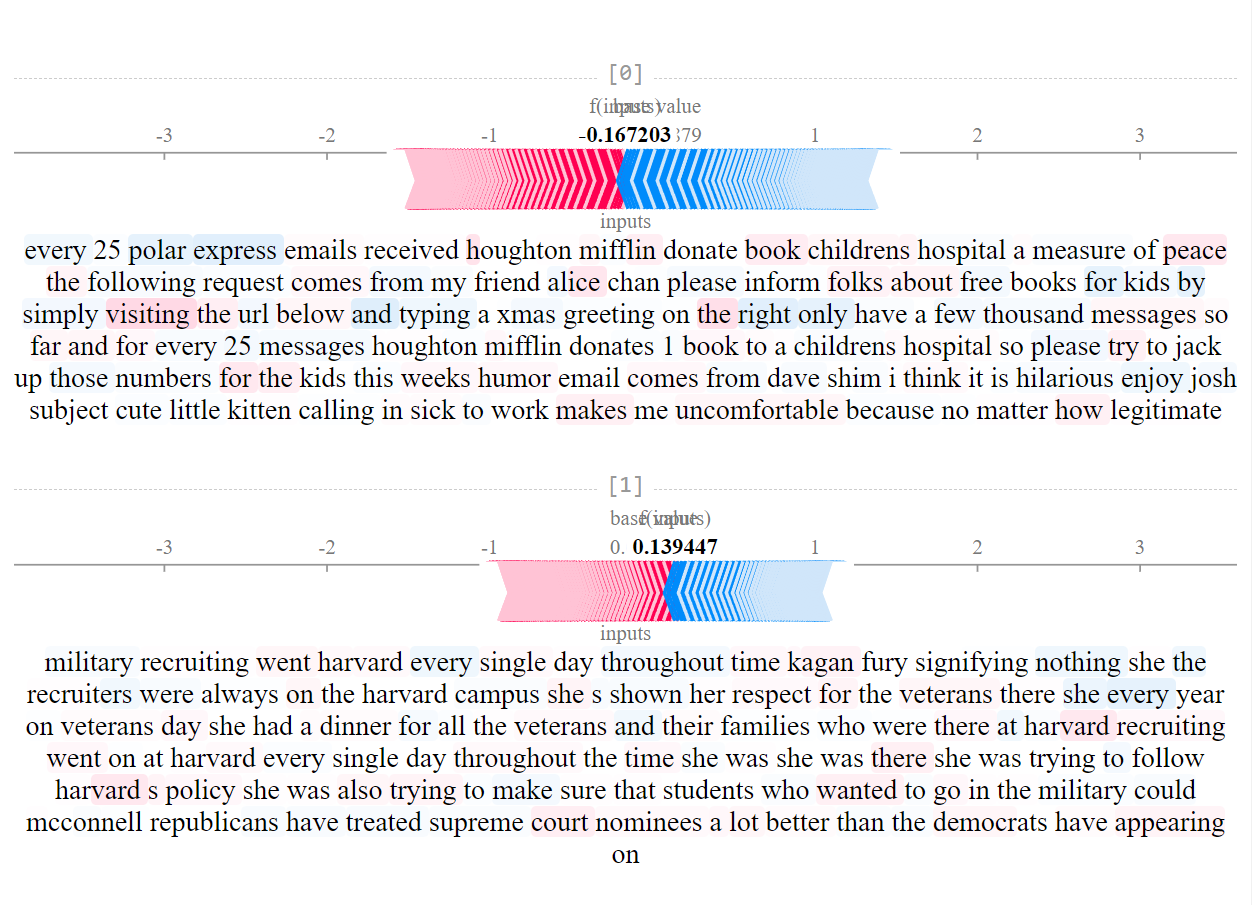
\includegraphics[width=\textwidth]{figs/one_TF/roberta-b.png}
        \caption{{RoBERTa}\textsubscript{B}}
    \end{subfigure}
    \hspace{\fill} % maximize horizontal separation
    \begin{subfigure}[t]{0.4\textwidth}
        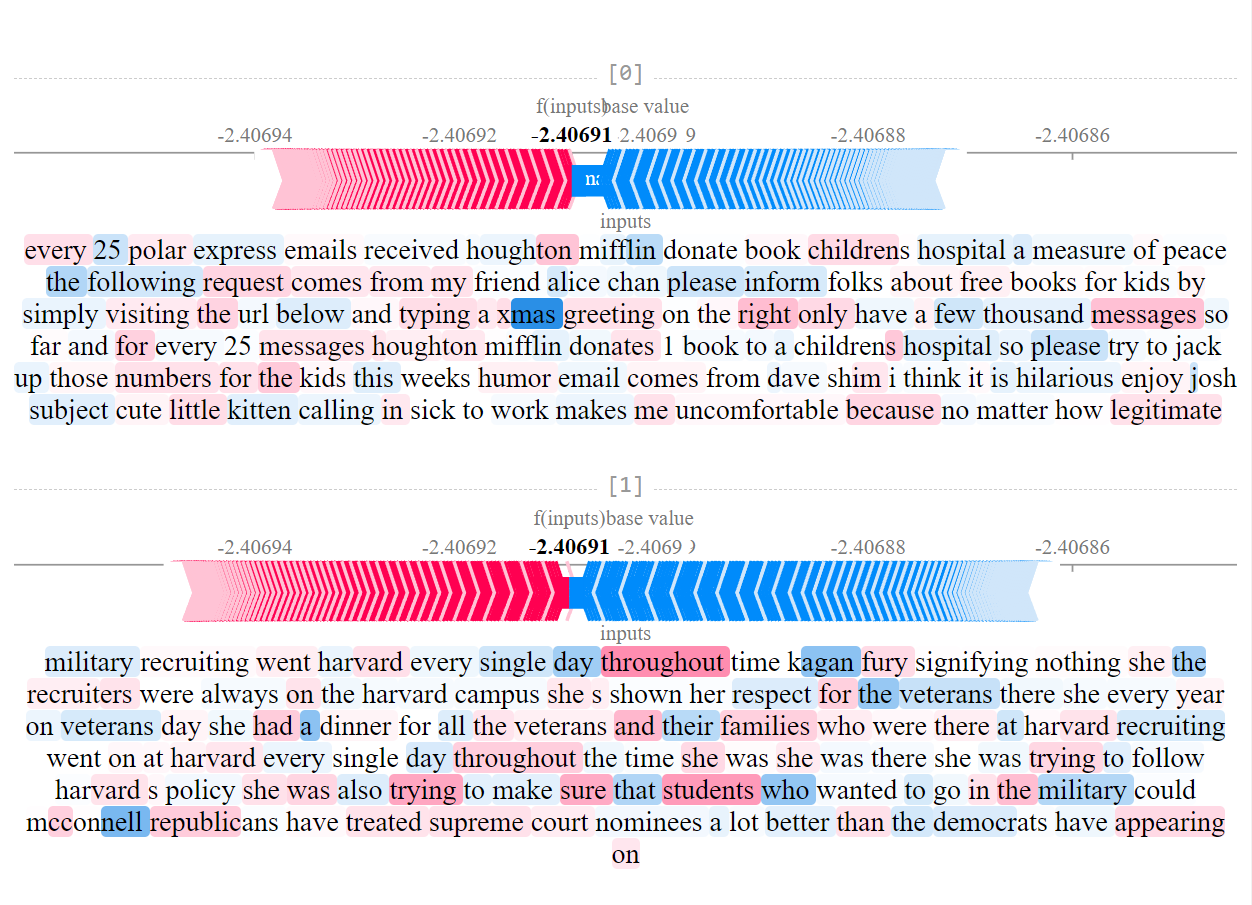
\includegraphics[width=\linewidth]{figs/one_TF/roberta-l.png}
        \caption{{RoBERTa}\textsubscript{L}}
    \end{subfigure}


% \end{figure}
% \begin{figure}[h]\ContinuedFloat
%     \captionsetup[subfigure]{justification=Centering}

    % DeBERTa (BASE / LARGE)
    % \bigskip % more vertical separation
    \begin{subfigure}[t]{0.4\textwidth}
        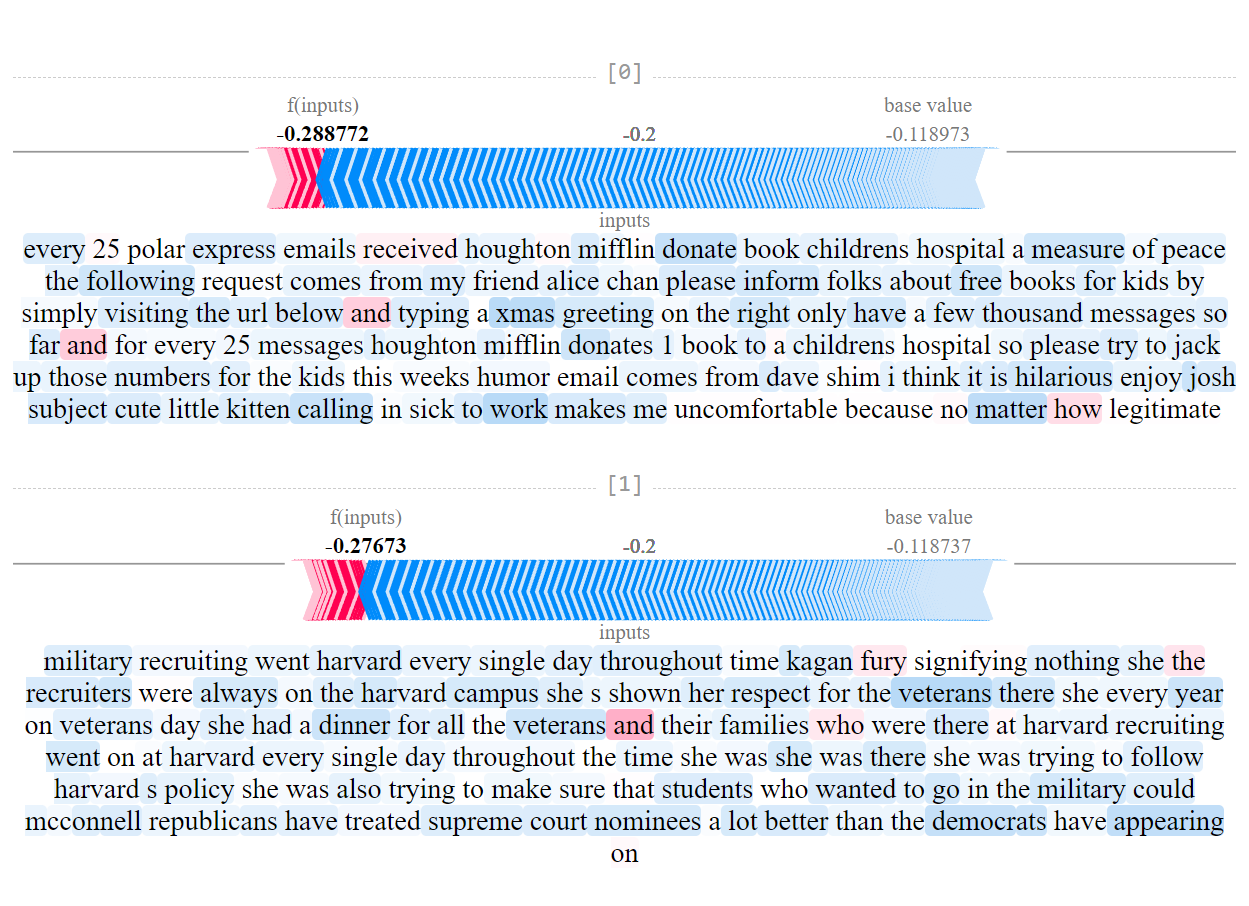
\includegraphics[width=\textwidth]{figs/one_TF/deberta-b.png}
        \caption{{DeBERTa}\textsubscript{B}}
    \end{subfigure}
    \hspace{\fill} % maximize horizontal separation
    \begin{subfigure}[t]{0.4\textwidth}
        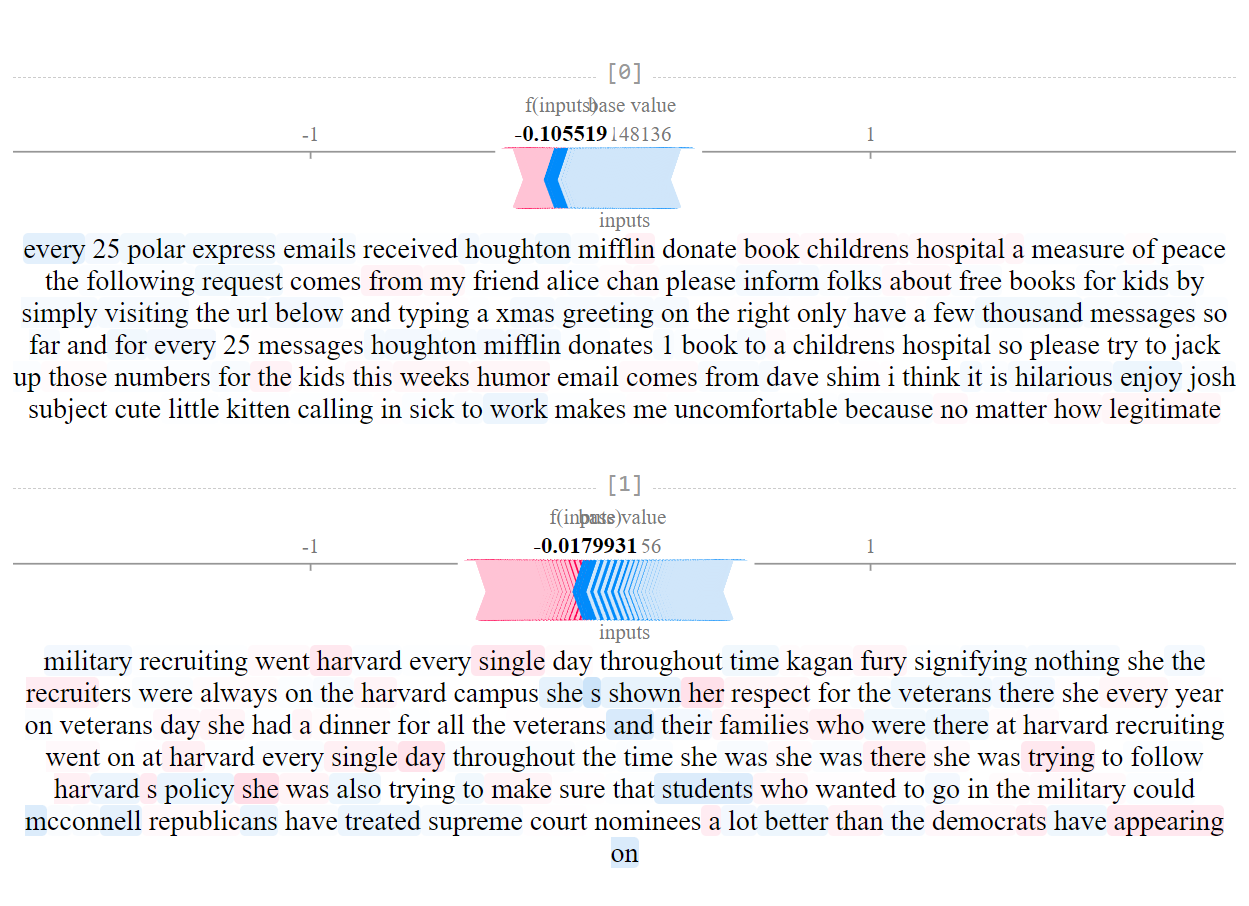
\includegraphics[width=\linewidth]{figs/one_TF/deberta-l.png}
        \caption{{DeBERTa}\textsubscript{L}}
    \end{subfigure}    
    
    \caption{Valores Shapley de cada modelo. Los subíndices utilizados para cada modelo $M$ indican respectivamente $M_{\text{B}}$: BASE; $M_{\text{L}}$: LARGE; $M_{C}$: CASED; $M_{\text{U}}$: UNCASED; $M_{\text{ML}}$: MULTILINGUAL.}
\end{figure}



\clearpage
\subsection{Politifact-Snopes All Evidences}
\label{fig:shap-ps-all-annex}

\begin{figure}[!h]
    \captionsetup[subfigure]{justification=Centering}
    % BERT BASE (UNCASED / CASED)
    \begin{subfigure}[t]{0.4\textwidth}
        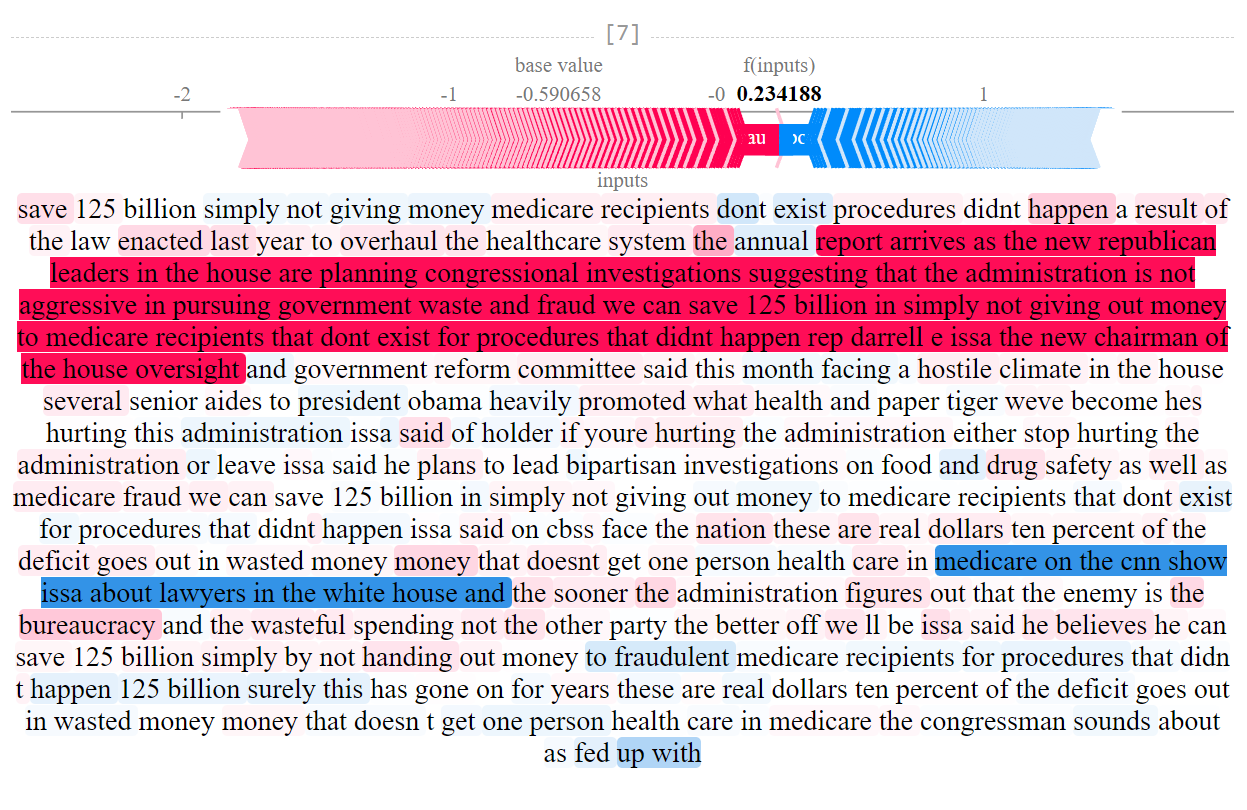
\includegraphics[width=\textwidth]{figs/all_F/bert-b-u.png}
        \caption{{BERT}\textsubscript{B, U}}
    \end{subfigure}
    \hspace{\fill} % maximize horizontal separation
    \begin{subfigure}[t]{0.4\textwidth}
        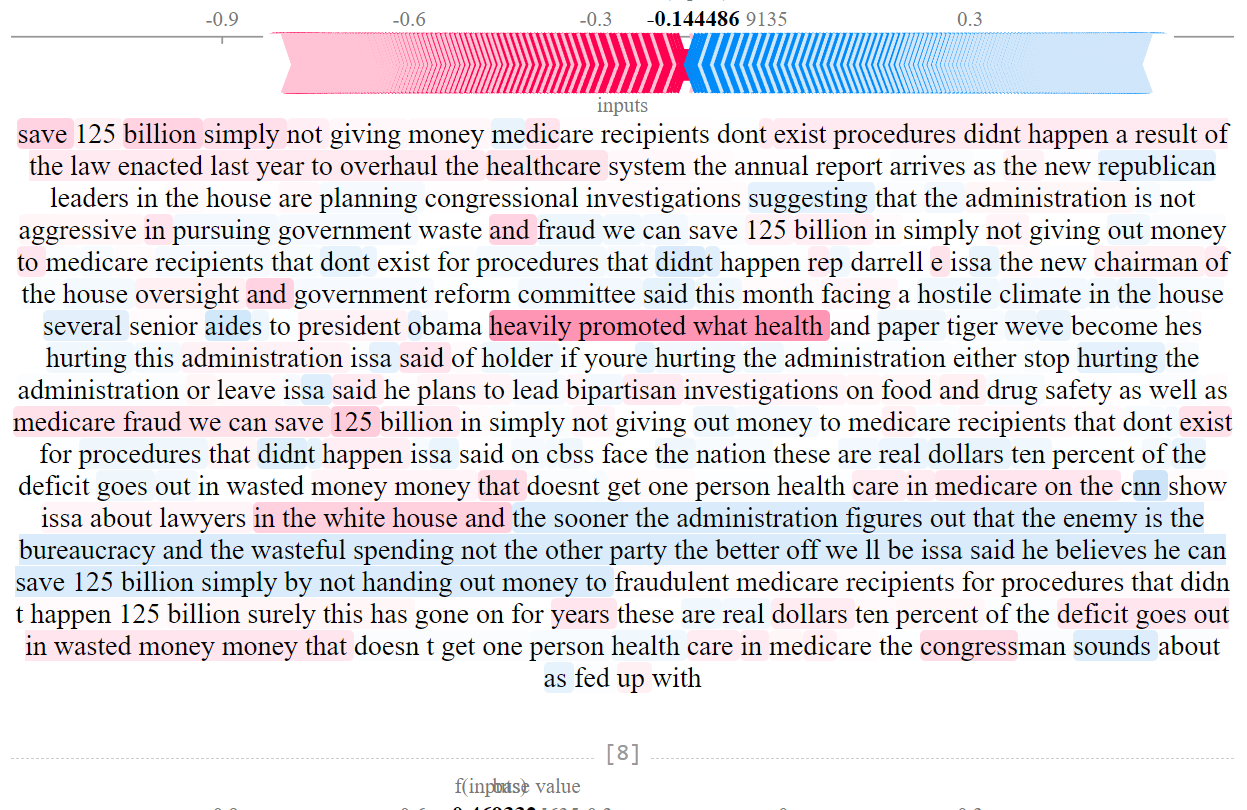
\includegraphics[width=\linewidth]{figs/all_F/bert-b-c.png}
        \caption{{BERT}\textsubscript{B, C}}
    \end{subfigure}


% \end{figure}
% \begin{figure}[h]\ContinuedFloat
%     \captionsetup[subfigure]{justification=Centering}

    % BERT BASE MULTILINGUAL (UNCASED / CASED)
    \begin{subfigure}[t]{0.4\textwidth}
        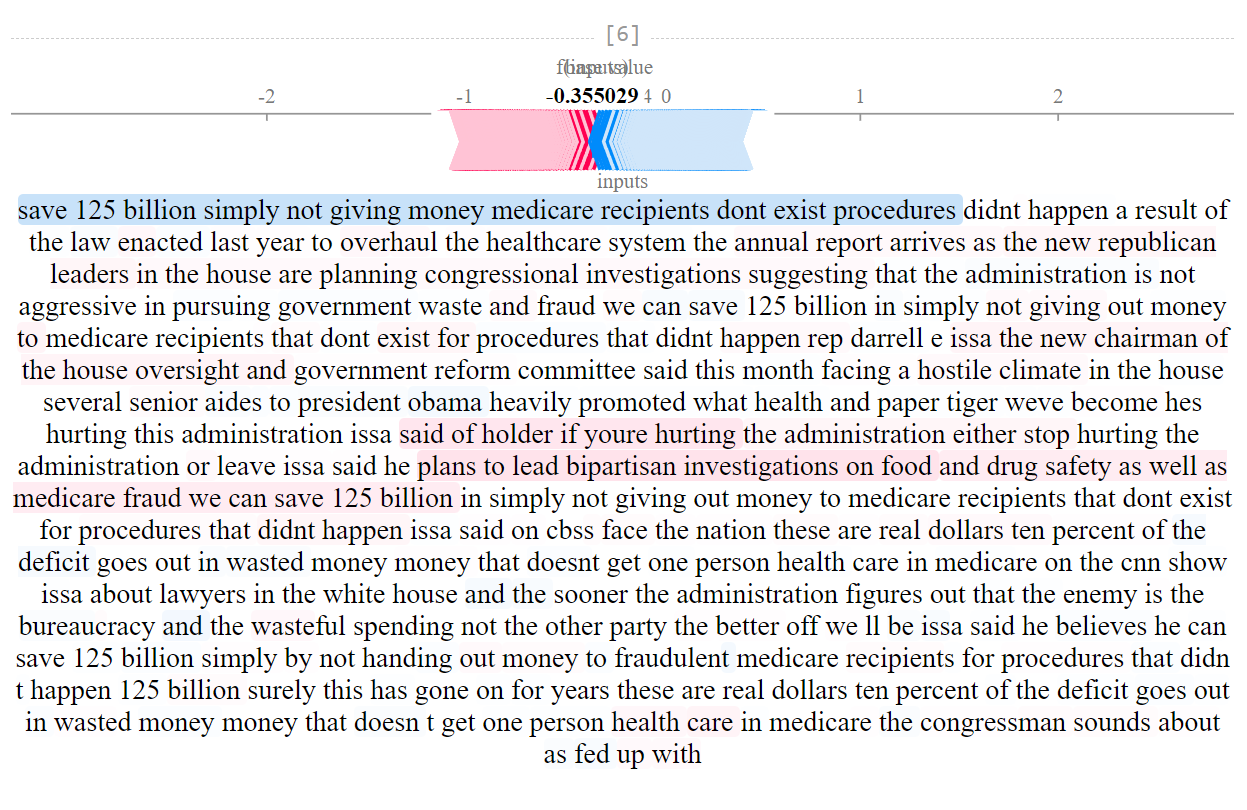
\includegraphics[width=\textwidth]{figs/all_F/bert-b-ml-u.png}
        \caption{{BERT}\textsubscript{B, U, ML}}
    \end{subfigure}
    \hspace{\fill} % maximize horizontal separation
    \begin{subfigure}[t]{0.4\textwidth}
        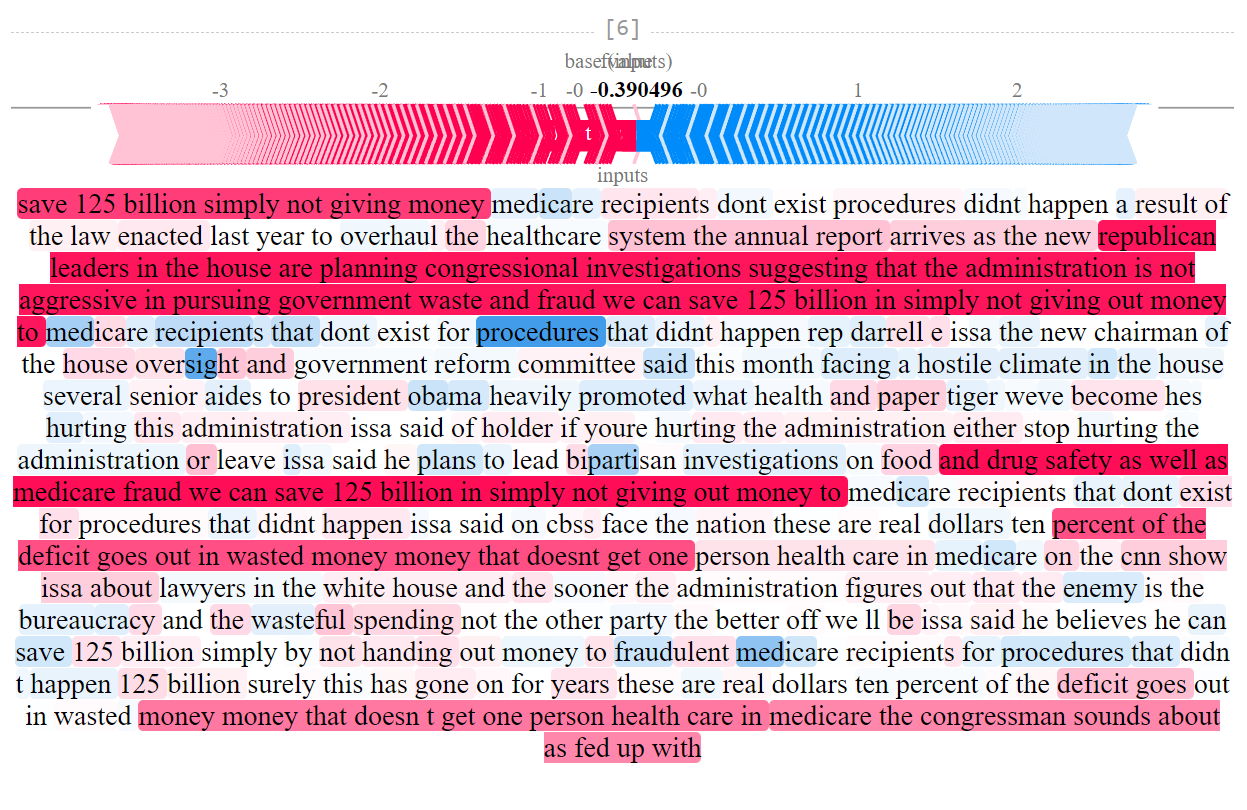
\includegraphics[width=\linewidth]{figs/all_F/bert-b-ml-c.png}
        \caption{{BERT}\textsubscript{B, C, ML}}
    \end{subfigure}


% \end{figure}
% \begin{figure}[h]\ContinuedFloat
%     \captionsetup[subfigure]{justification=Centering}

    % BERT LARGE (UNCASED / CASED)
    \begin{subfigure}[t]{0.4\textwidth}
        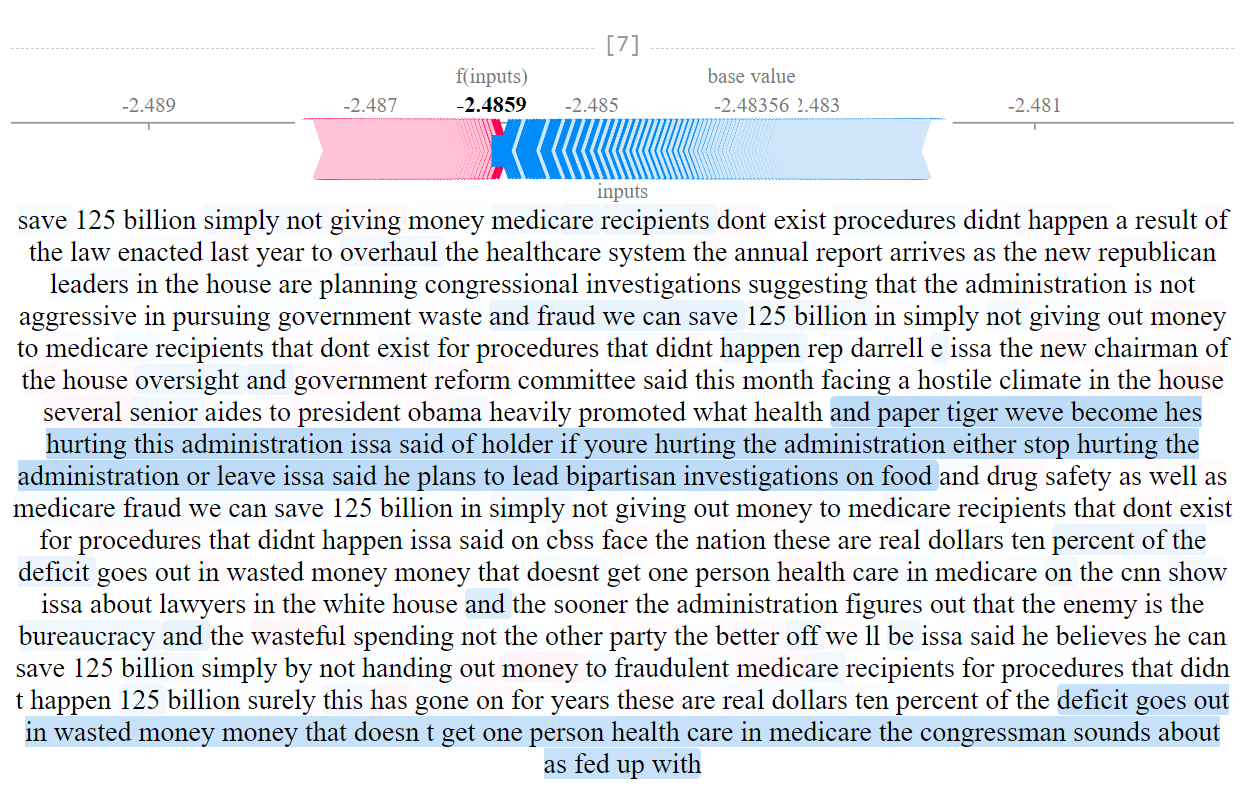
\includegraphics[width=\textwidth]{figs/all_F/bert-l-u.png}
        \caption{{BERT}\textsubscript{L, U}}
    \end{subfigure}
    \hspace{\fill} % maximize horizontal separation
    \begin{subfigure}[t]{0.4\textwidth}
        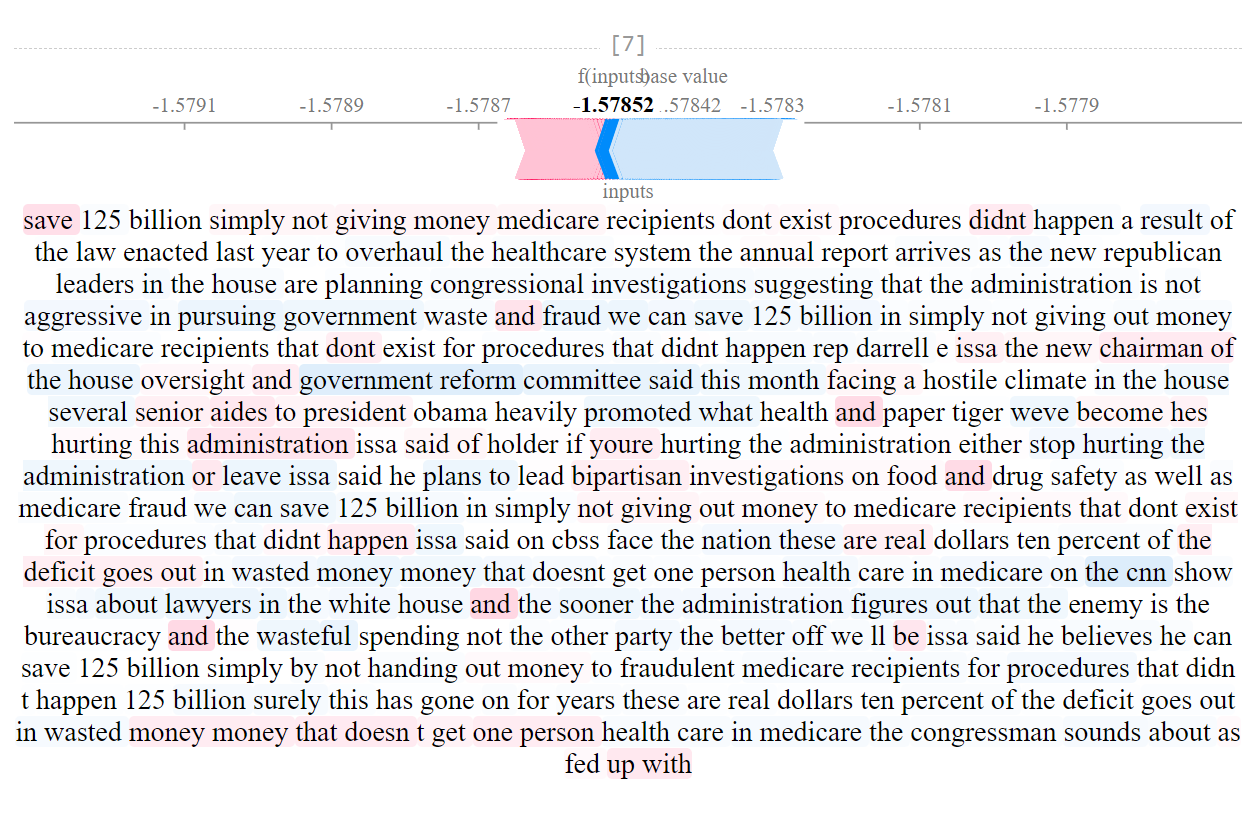
\includegraphics[width=\linewidth]{figs/all_F/bert-l-c.png}
        \caption{{BERT}\textsubscript{L, C}}
    \end{subfigure}


% \end{figure}
% \begin{figure}[h]\ContinuedFloat
%     \captionsetup[subfigure]{justification=Centering}

    % DistilBERT BASE (CASED / CASED MULTILINGUAL)
    \begin{subfigure}[t]{0.4\textwidth}
        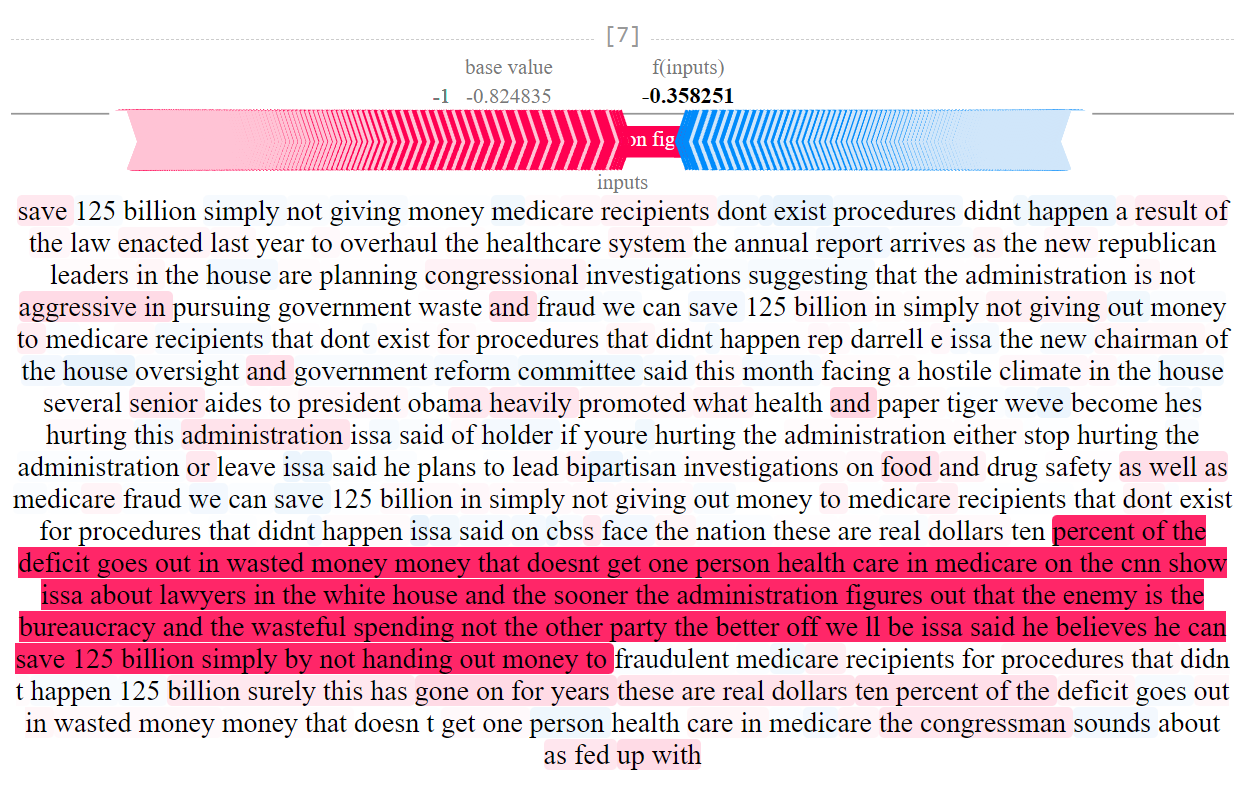
\includegraphics[width=\textwidth]{figs/all_F/distil-b-c.png}
        \caption{{DistilBERT}\textsubscript{B, C}}
    \end{subfigure}
    \hspace{\fill} % maximize horizontal separation
    \begin{subfigure}[t]{0.4\textwidth}
        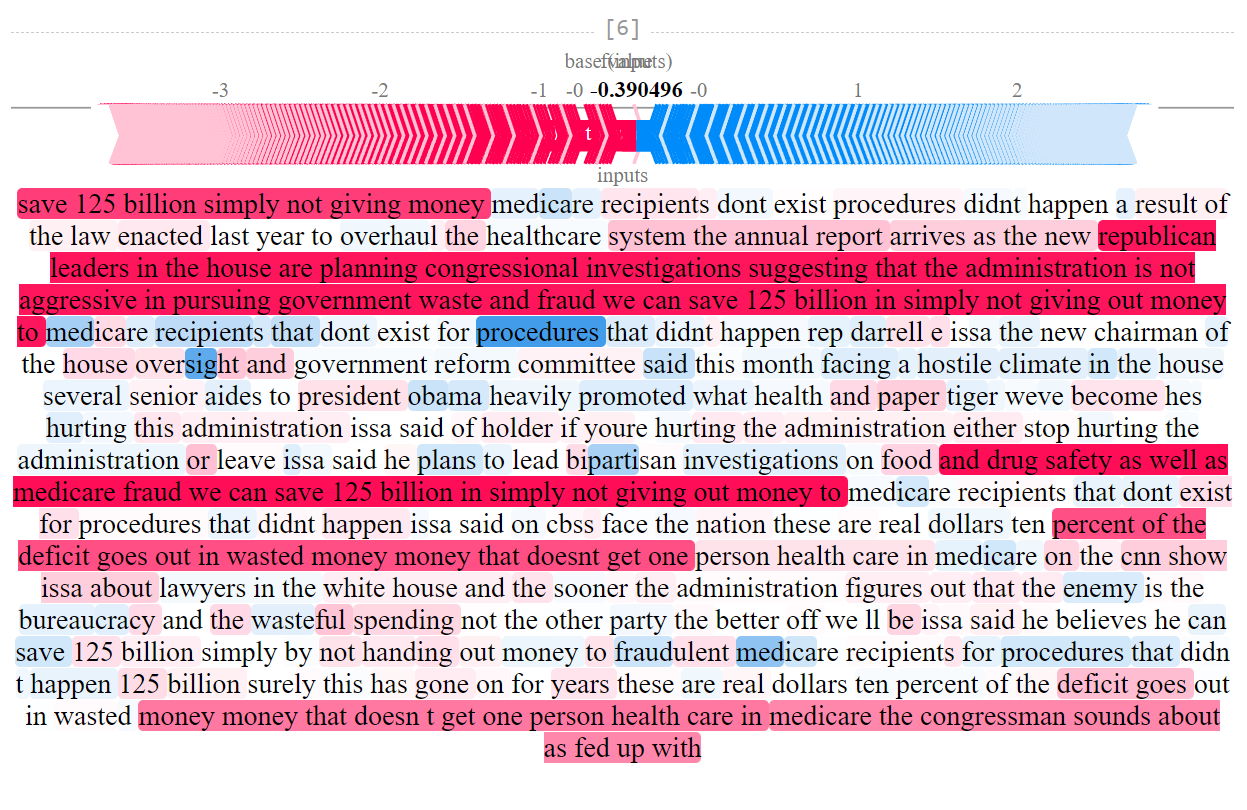
\includegraphics[width=\linewidth]{figs/all_F/bert-b-ml-c.png}
        \caption{{DistilBERT}\textsubscript{B, C, ML}}
    \end{subfigure}


\end{figure}
\begin{figure}[ht]\ContinuedFloat
    \captionsetup[subfigure]{justification=Centering}

    % RoBERTa (BASE / LARGE)
    \begin{subfigure}[t]{0.4\textwidth}
        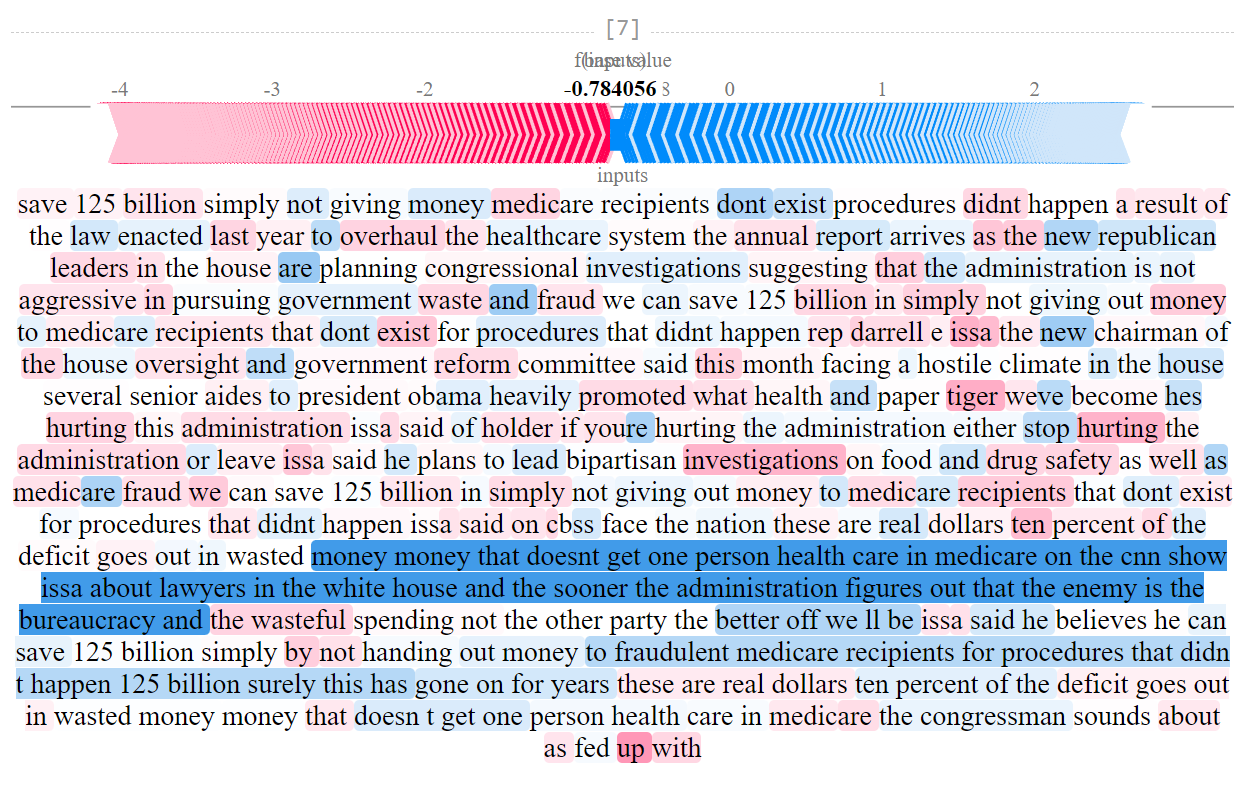
\includegraphics[width=\textwidth]{figs/all_F/roberta-b.png}
        \caption{{RoBERTa}\textsubscript{B}}
    \end{subfigure}
    \hspace{\fill} % maximize horizontal separation
    \begin{subfigure}[t]{0.4\textwidth}
        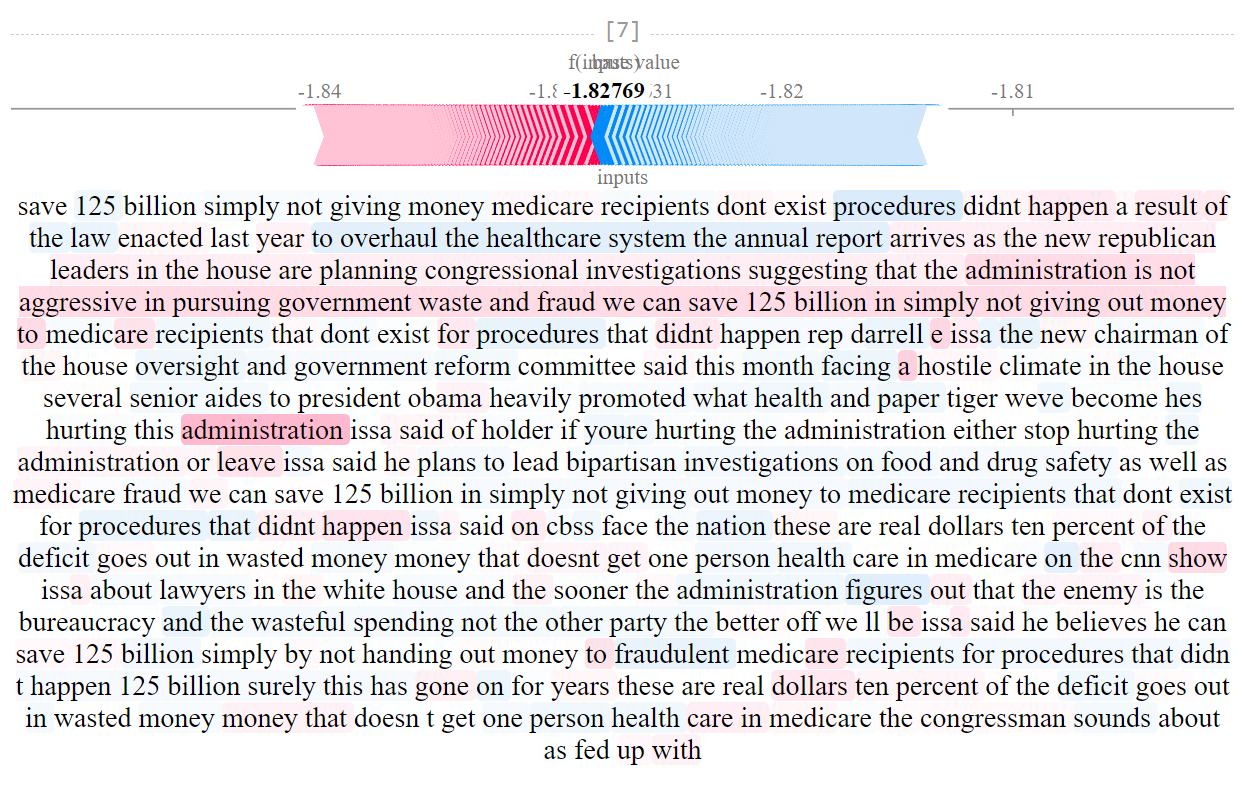
\includegraphics[width=\linewidth]{figs/all_F/roberta-l.png}
        \caption{{RoBERTa}\textsubscript{L}}
    \end{subfigure}


% \end{figure}
% \begin{figure}[h]\ContinuedFloat
%     \captionsetup[subfigure]{justification=Centering}

    % DeBERTa (BASE / LARGE)
    % \bigskip % more vertical separation
    \begin{subfigure}[t]{0.4\textwidth}
        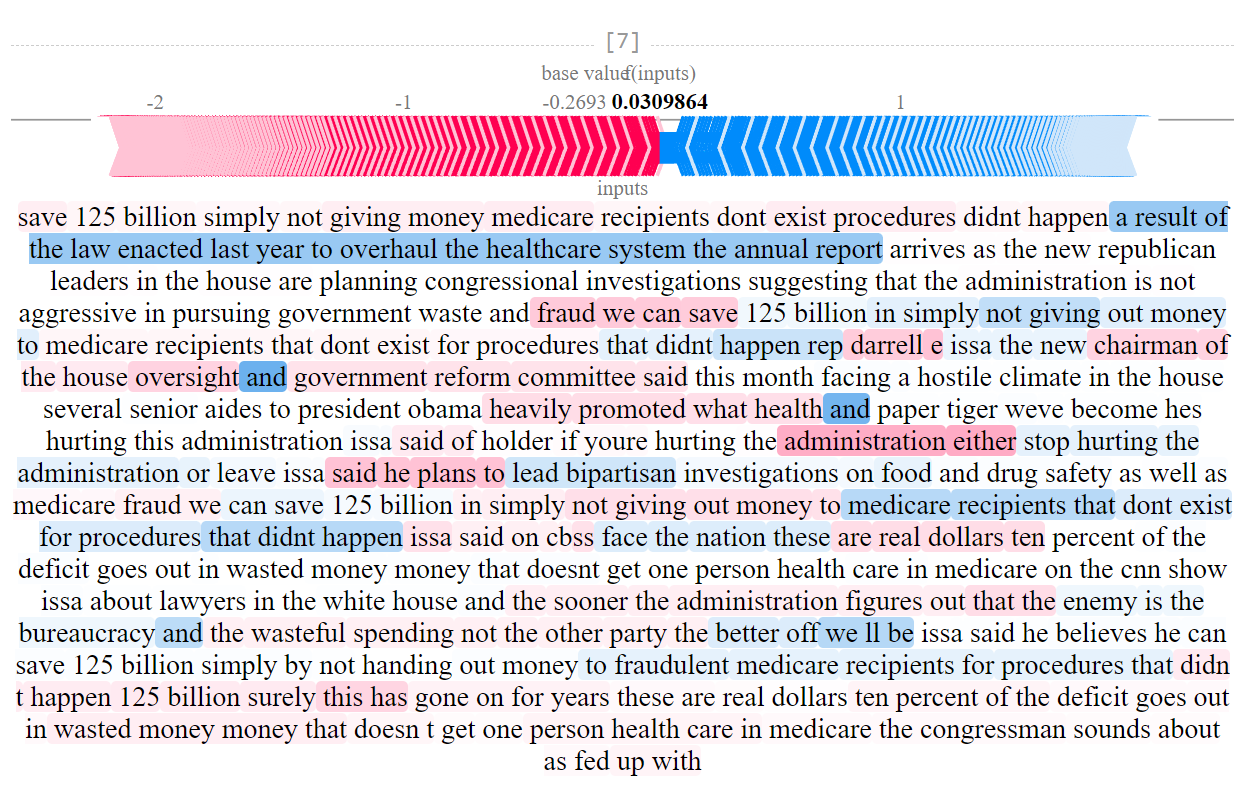
\includegraphics[width=\textwidth]{figs/all_F/deberta-b.png}
        \caption{{DeBERTa}\textsubscript{B}}
    \end{subfigure}
    \hspace{\fill} % maximize horizontal separation
    \begin{subfigure}[t]{0.4\textwidth}
        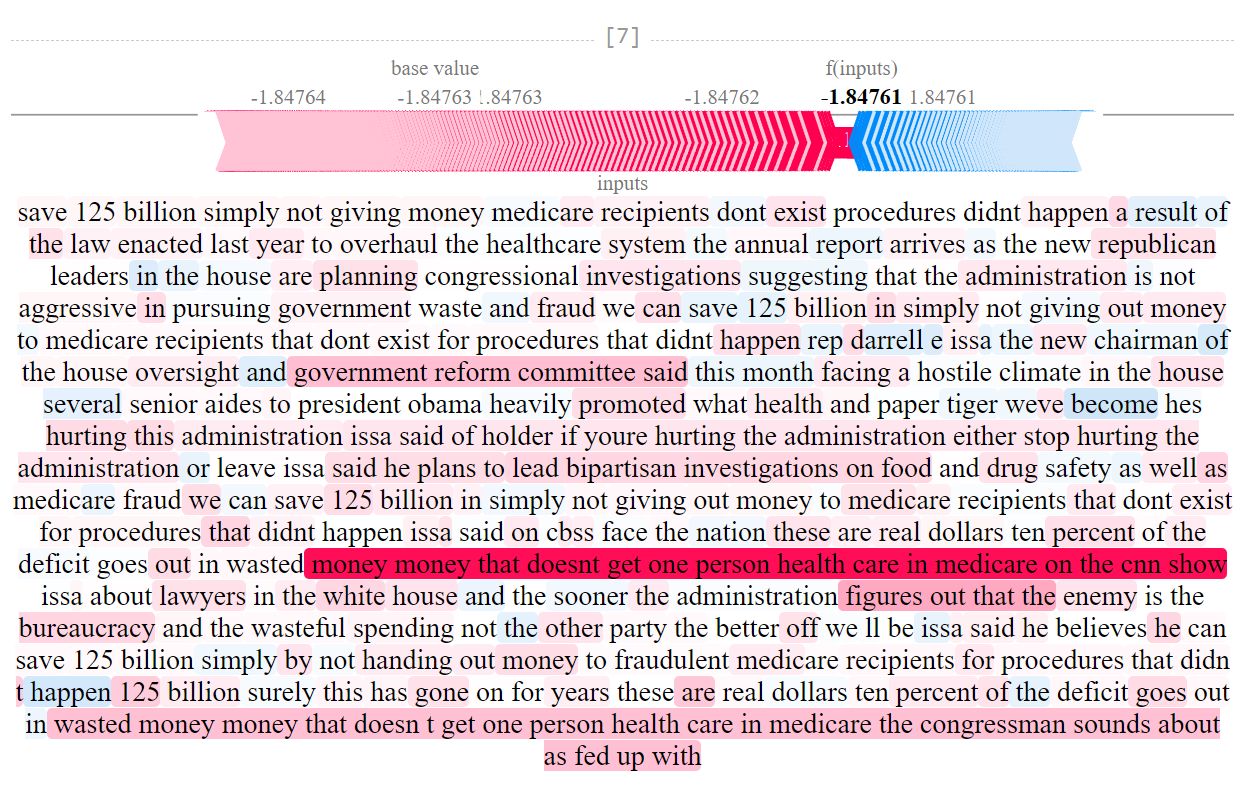
\includegraphics[width=\linewidth]{figs/all_F/deberta-l.png}
        \caption{{DeBERTa}\textsubscript{L}}
    \end{subfigure}    
    
    \caption{Valores Shapley de cada modelo. Los subíndices utilizados para cada modelo $M$ indican respectivamente $M_{\text{B}}$: BASE; $M_{\text{L}}$: LARGE; $M_{C}$: CASED; $M_{\text{U}}$: UNCASED; $M_{\text{ML}}$: MULTILINGUAL.}
\end{figure}


\clearpage
\subsection{News}
\label{fig:shap-news-annex}

\begin{figure}[!h]
    \captionsetup[subfigure]{justification=Centering}
    % BERT BASE (UNCASED / CASED)
    \begin{subfigure}[t]{0.35\textwidth}
        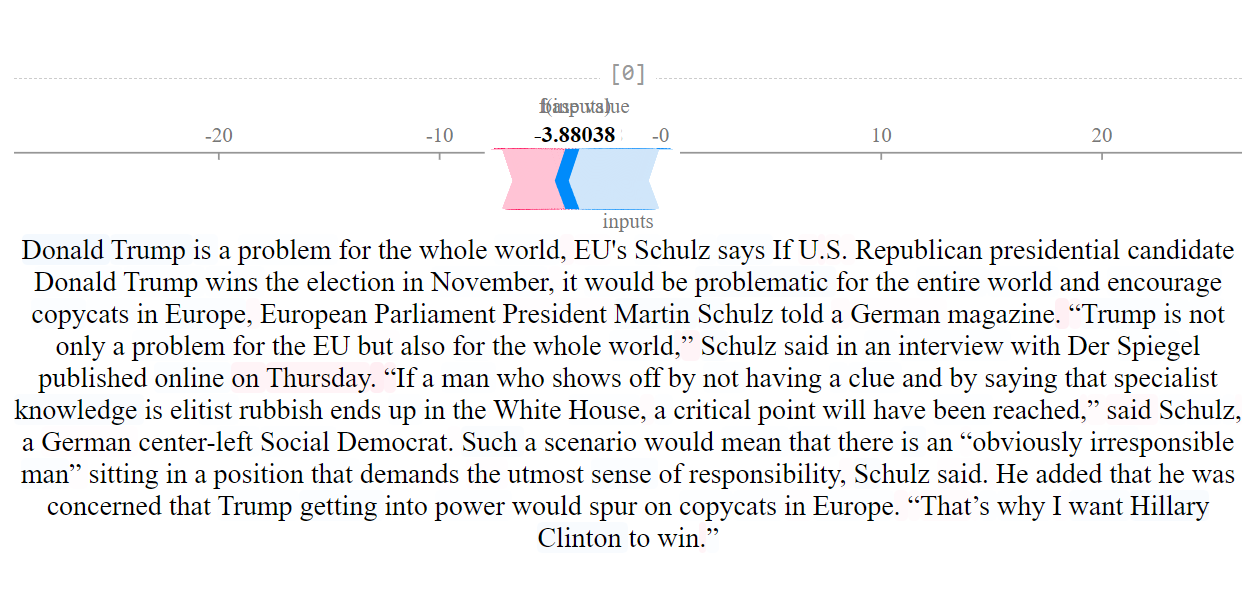
\includegraphics[width=\textwidth]{figs/news_T/bert-b-u.png}
        \caption{{BERT}\textsubscript{B, U}}
    \end{subfigure}
    \hspace{\fill} % maximize horizontal separation
    \begin{subfigure}[t]{0.35\textwidth}
        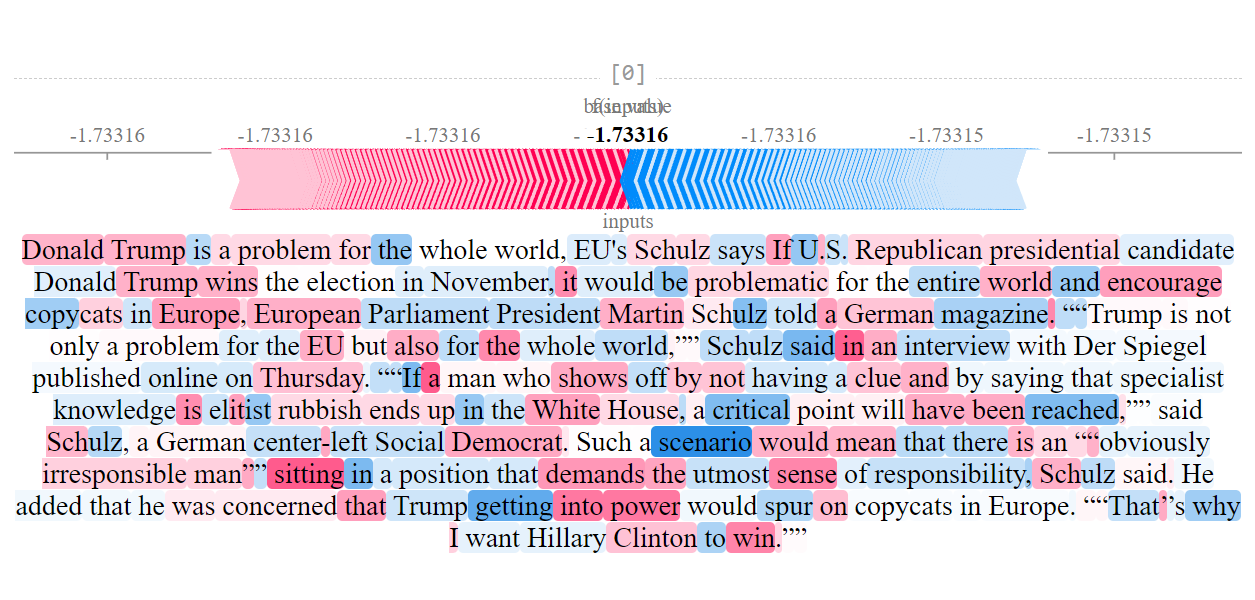
\includegraphics[width=\linewidth]{figs/news_T/bert-b-c.png}
        \caption{{BERT}\textsubscript{B, C}}
    \end{subfigure}


% \end{figure}
% \begin{figure}[h]\ContinuedFloat
%     \captionsetup[subfigure]{justification=Centering}

    % BERT BASE MULTILINGUAL (UNCASED / CASED)
    \begin{subfigure}[t]{0.35\textwidth}
        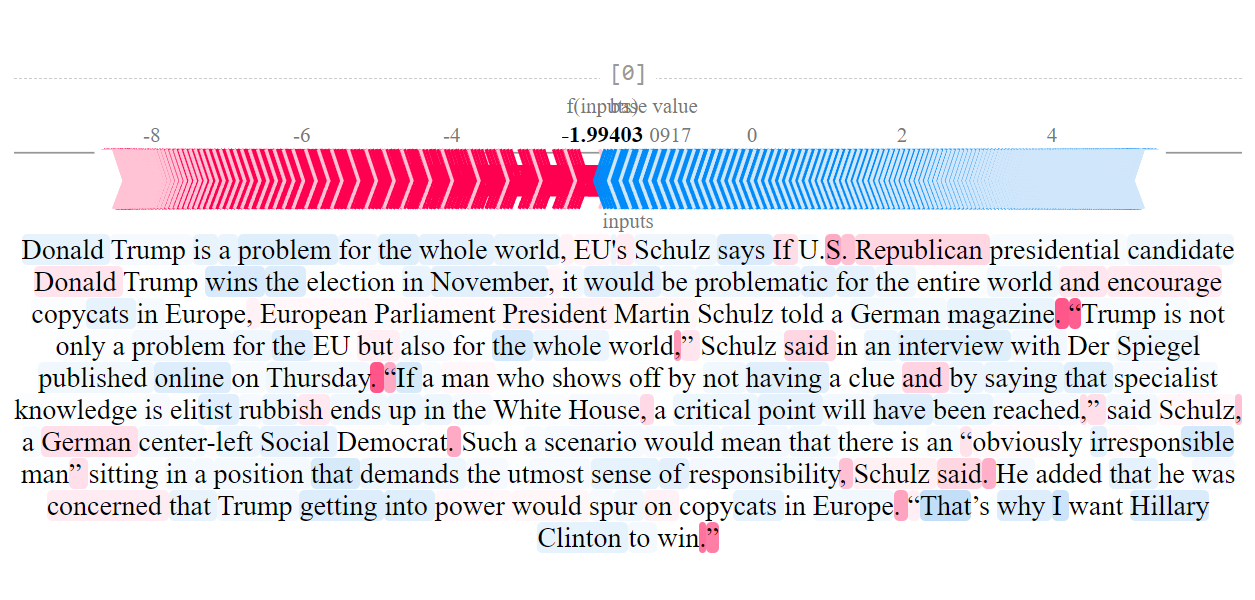
\includegraphics[width=\textwidth]{figs/news_T/bert-b-ml-u.png}
        \caption{{BERT}\textsubscript{B, U, ML}}
    \end{subfigure}
    \hspace{\fill} % maximize horizontal separation
    \begin{subfigure}[t]{0.35\textwidth}
        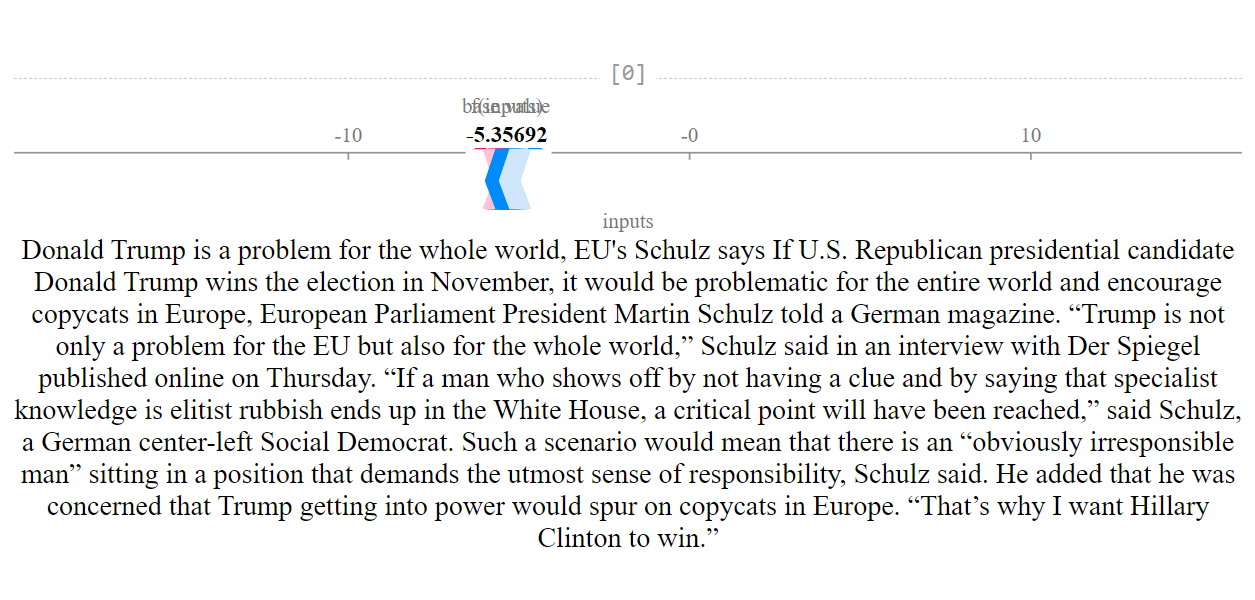
\includegraphics[width=\linewidth]{figs/news_T/bert-b-ml-c.png}
        \caption{{BERT}\textsubscript{B, C, ML}}
    \end{subfigure}


% \end{figure}
% \begin{figure}[h]\ContinuedFloat
%     \captionsetup[subfigure]{justification=Centering}

    % BERT LARGE (UNCASED / CASED)
    \begin{subfigure}[t]{0.35\textwidth}
        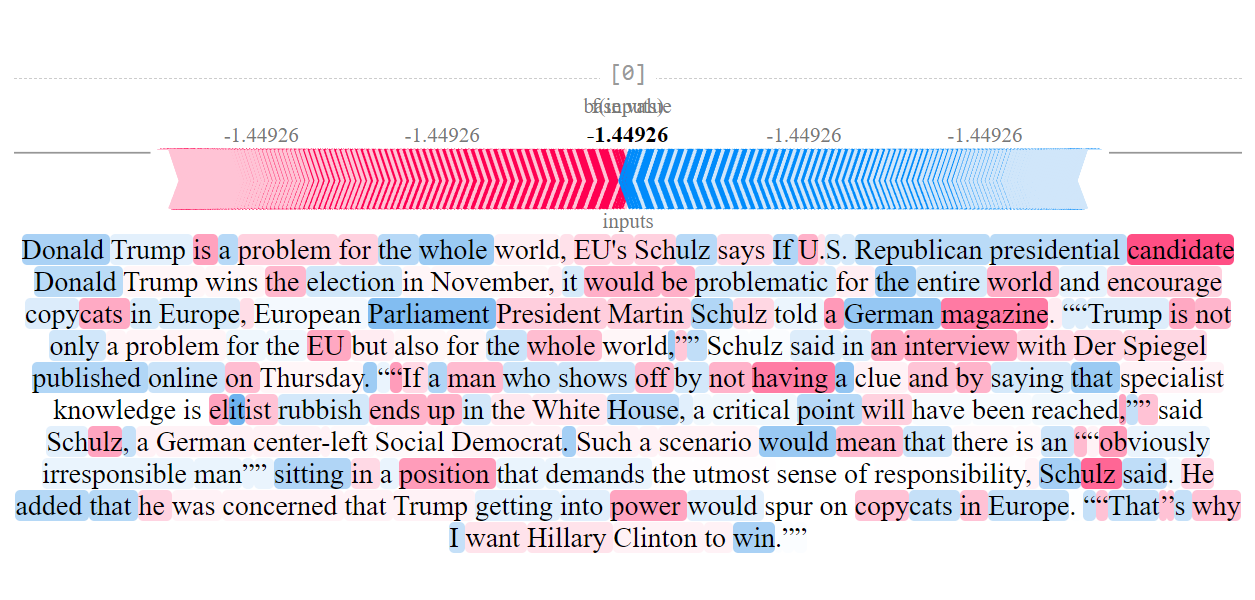
\includegraphics[width=\textwidth]{figs/news_T/bert-l-u.png}
        \caption{{BERT}\textsubscript{L, U}}
    \end{subfigure}
    \hspace{\fill} % maximize horizontal separation
    \begin{subfigure}[t]{0.35\textwidth}
        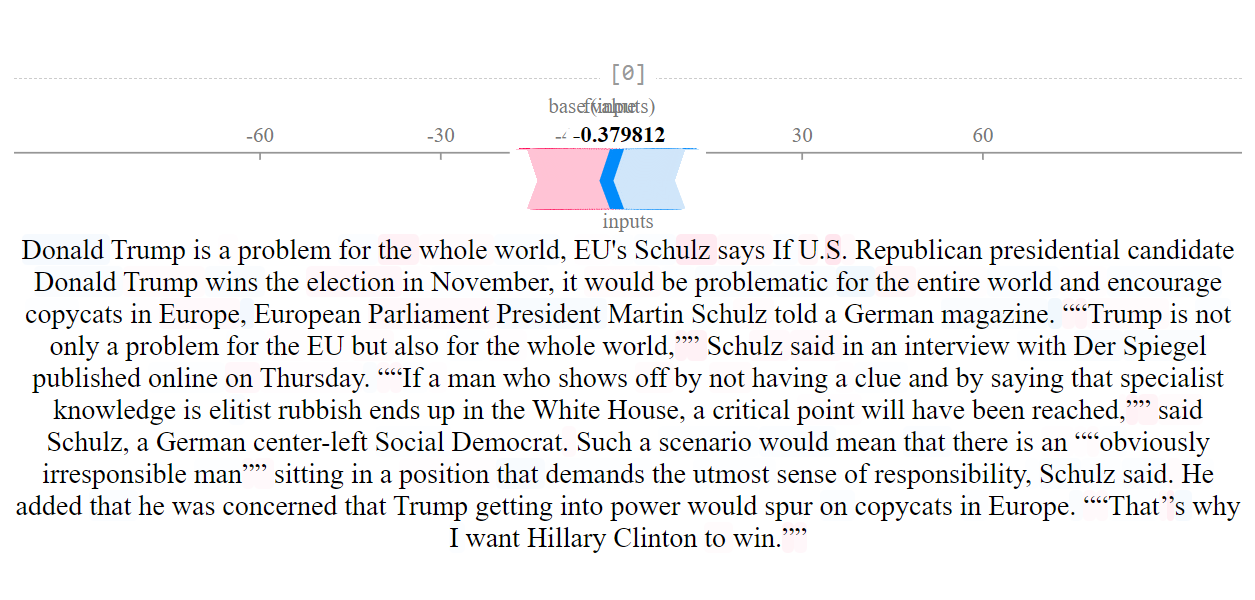
\includegraphics[width=\linewidth]{figs/news_T/bert-l-c.png}
        \caption{{BERT}\textsubscript{L, C}}
    \end{subfigure}


% \end{figure}
% \begin{figure}[h]\ContinuedFloat
%     \captionsetup[subfigure]{justification=Centering}

    % DistilBERT BASE (CASED / CASED MULTILINGUAL)
    \begin{subfigure}[t]{0.35\textwidth}
        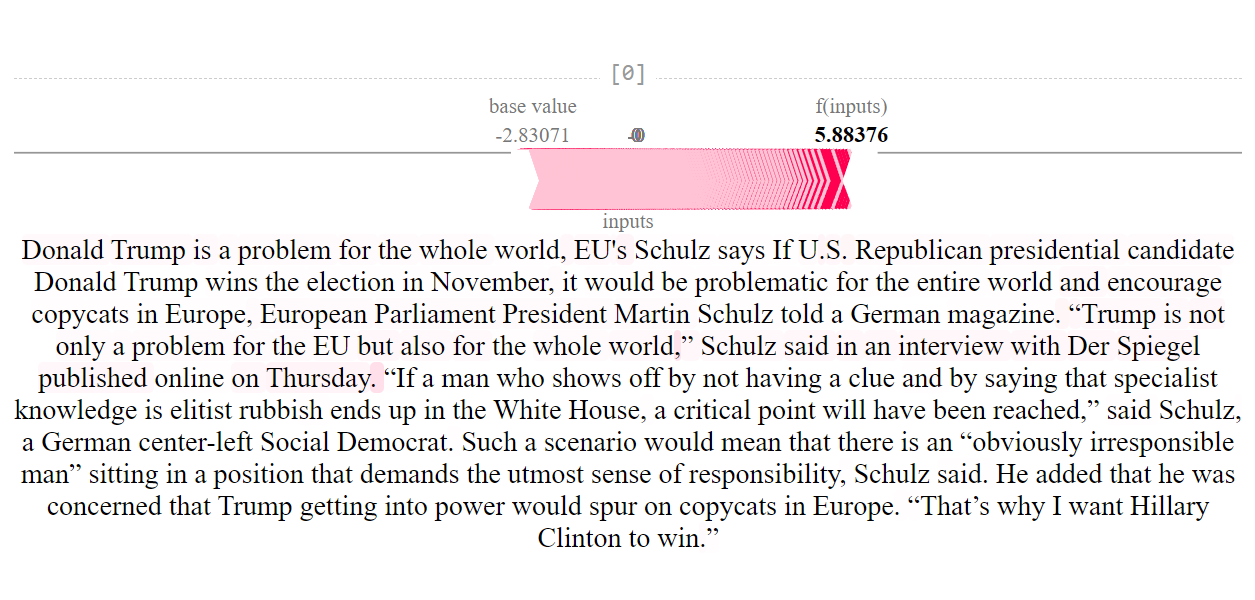
\includegraphics[width=\textwidth]{figs/news_T/distil-b-c.png}
        \caption{{DistilBERT}\textsubscript{B, C}}
    \end{subfigure}
    \hspace{\fill} % maximize horizontal separation
    \begin{subfigure}[t]{0.35\textwidth}
        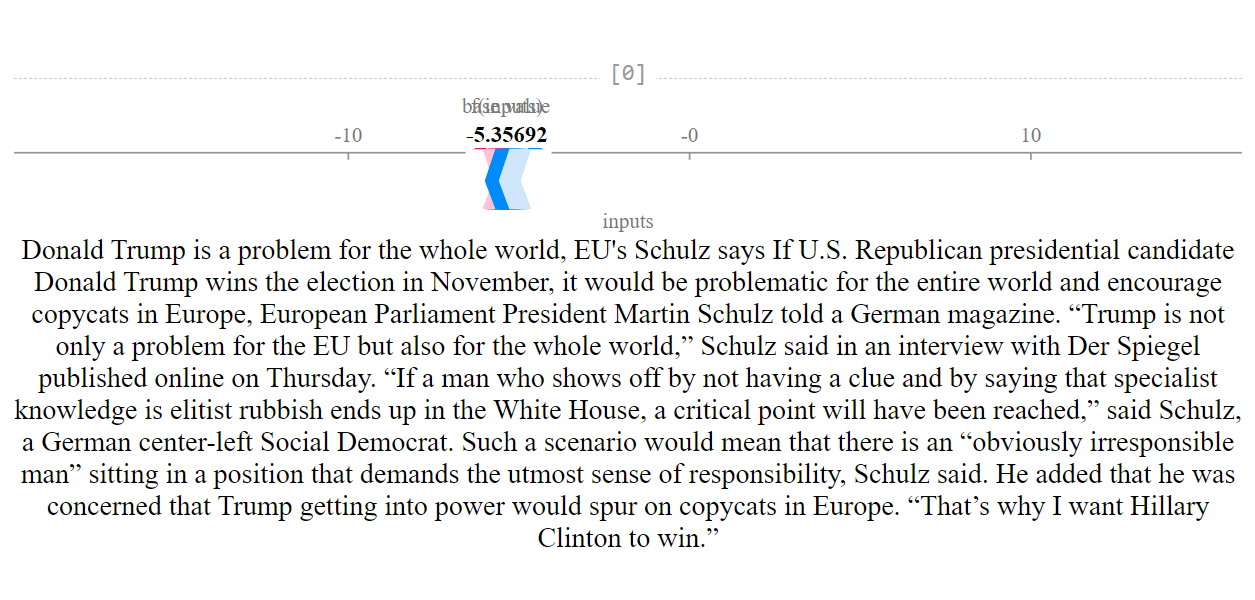
\includegraphics[width=\linewidth]{figs/news_T/bert-b-ml-c.png}
        \caption{{DistilBERT}\textsubscript{B, C, ML}}
    \end{subfigure}


% \end{figure}
% \begin{figure}[!ht]\ContinuedFloat
%     \captionsetup[subfigure]{justification=Centering}

    % RoBERTa (BASE / LARGE)
    \begin{subfigure}[t]{0.35\textwidth}
        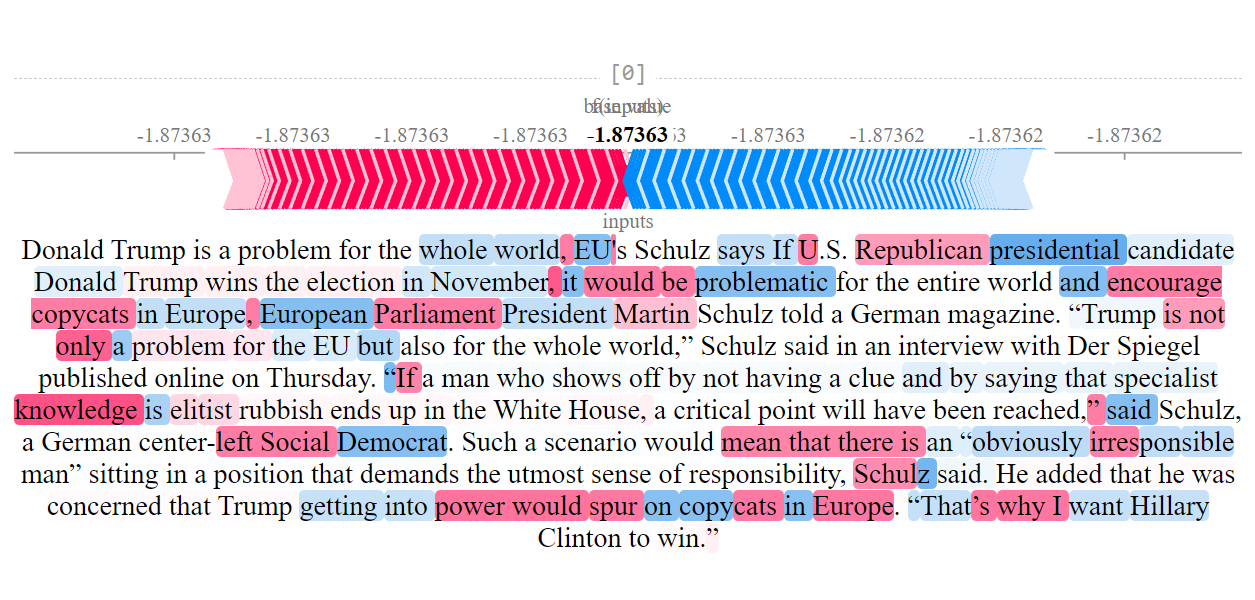
\includegraphics[width=\textwidth]{figs/news_T/roberta-b.png}
        \caption{{RoBERTa}\textsubscript{B}}
    \end{subfigure}
    \hspace{\fill} % maximize horizontal separation
    \begin{subfigure}[t]{0.35\textwidth}
        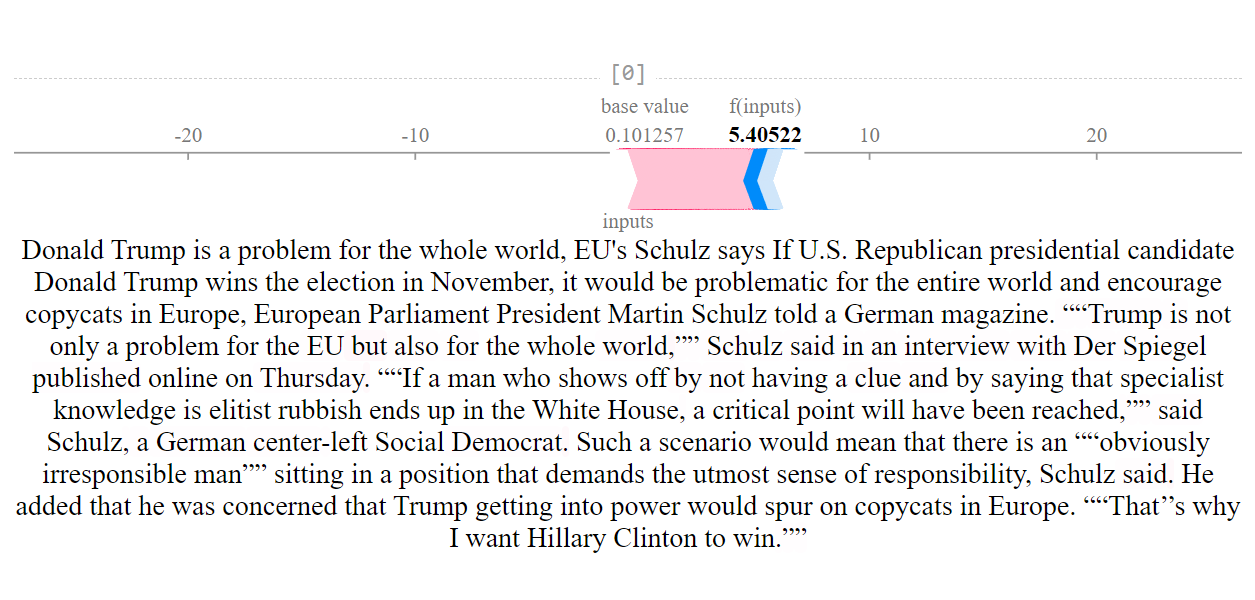
\includegraphics[width=\linewidth]{figs/news_T/roberta-l.png}
        \caption{{RoBERTa}\textsubscript{L}}
    \end{subfigure}


% \end{figure}
% \begin{figure}[h]\ContinuedFloat
%     \captionsetup[subfigure]{justification=Centering}

    % DeBERTa (BASE / LARGE)
    % \bigskip % more vertical separation
    \begin{subfigure}[t]{0.35\textwidth}
        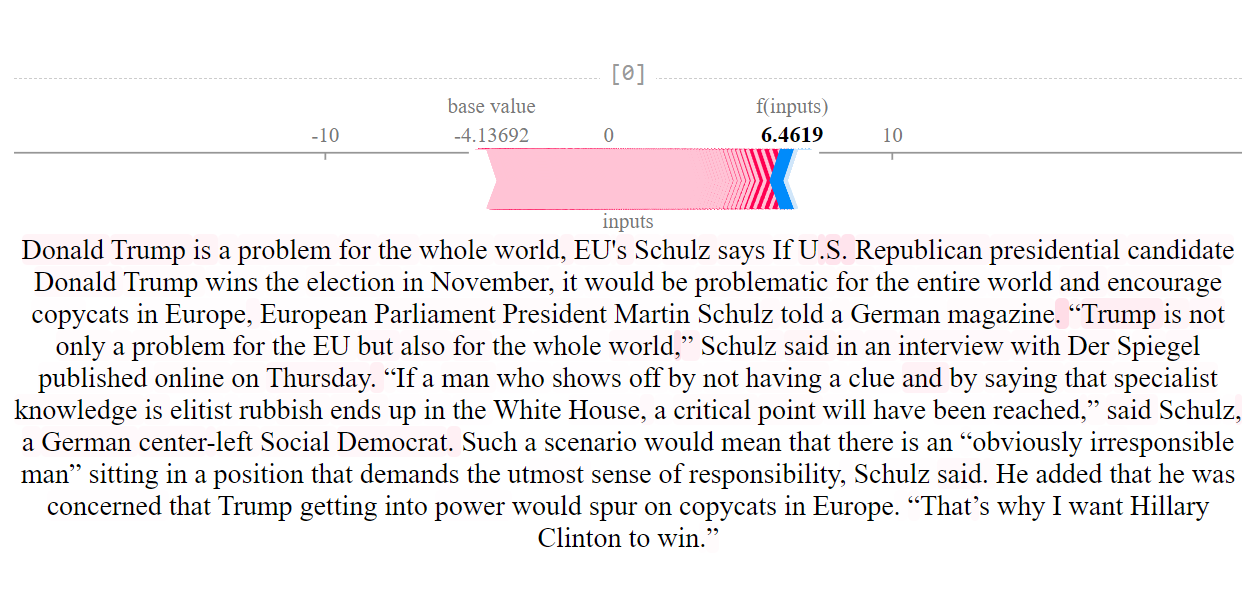
\includegraphics[width=\textwidth]{figs/news_T/deberta-b.png}
        \caption{{DeBERTa}\textsubscript{B}}
    \end{subfigure}
    \hspace{\fill} % maximize horizontal separation
    \begin{subfigure}[t]{0.35\textwidth}
        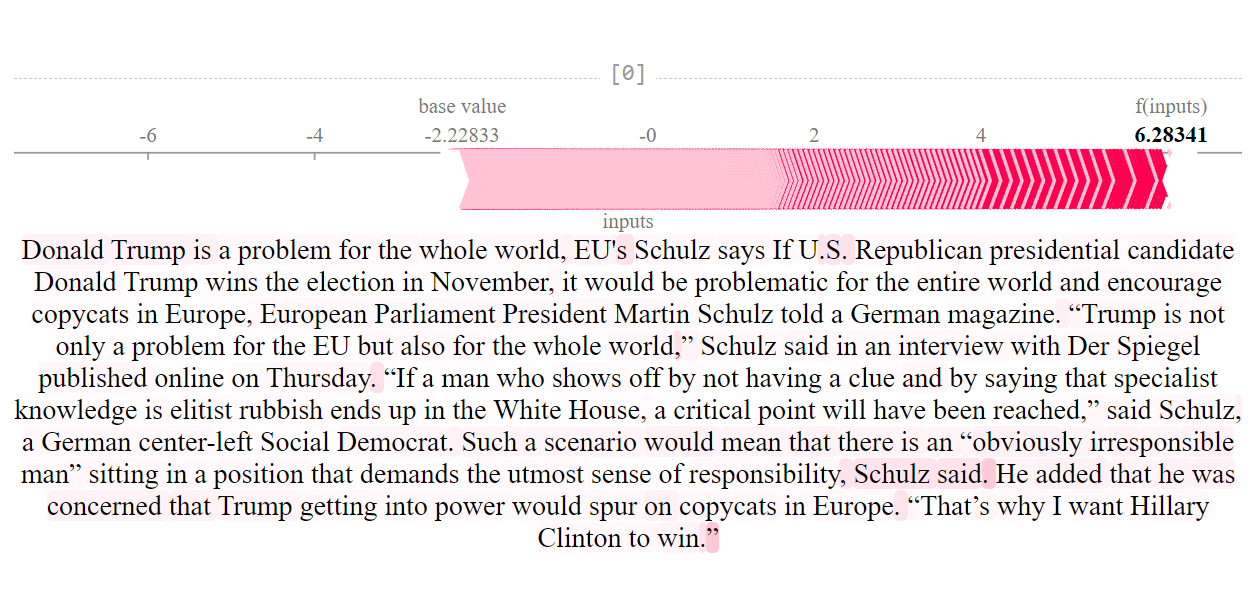
\includegraphics[width=\linewidth]{figs/news_T/deberta-l.png}
        \caption{{DeBERTa}\textsubscript{L}}
    \end{subfigure}    
    
    \caption{Valores Shapley de cada modelo. Los subíndices utilizados para cada modelo $M$ indican respectivamente $M_{\text{B}}$: BASE; $M_{\text{L}}$: LARGE; $M_{C}$: CASED; $M_{\text{U}}$: UNCASED; $M_{\text{ML}}$: MULTILINGUAL.}
\end{figure}

  



\end{document}

%%% Local Variables:
%%% mode: latex
%%% TeX-master: t
%%% End:
